\documentclass{vkr}
\usepackage[english, russian]{babel} % переносы
\usepackage{graphicx} % для вставки картинок
\graphicspath{{images/}} % путь к изображениям
\usepackage[hidelinks]{hyperref}
\usepackage{float} % определяет метод H для рисунка с переносом на следующую страницу, ели не помещается
\usepackage{pdflscape}
\addto{\captionsrussian}{\renewcommand{\refname}{СПИСОК ИСПОЛЬЗОВАННЫХ ИСТОЧНИКОВ}}
\usepackage{xltabular} % для вставки таблиц
\usepackage{makecell}
\renewcommand\theadfont{} % шрифт в /thead
\usepackage{array} % для определения новых типов столбцов таблиц
\newcolumntype{T}{>{\centering\arraybackslash}X} % новый тип столбца T - автоматическая ширина столбца с выравниванием по центру
\newcolumntype{R}{>{\raggedleft\arraybackslash}X} % новый тип столбца R - автоматическая ширина столбца с выравниванием по правому краю
\newcolumntype{C}[1]{>{\centering\let\newline\\\arraybackslash\hspace{0pt}}m{#1}} % новый тип столбца C - фиксированная ширина столбца с выравниванием по центру
%\newcolumntype{r}[1]{>{\raggedleft\arraybackslash}p{#1}} % новый тип столбца r - фиксированная ширина столбца с выравниванием по правому краю
\newcommand{\centrow}{\centering\arraybackslash} % командой \centrow можно центрировать одну ячейку (заголовок) в столбце типа X или p, оставив в оcтальных ячейках другой тип выравнивания
\newcommand{\finishhead}{\endhead\hline\endlastfoot}
\newcommand{\continuecaption}[1]{\captionsetup{labelformat=empty} \caption[]{#1}\\ \hline }
\usepackage{etoolbox}
\AtBeginEnvironment{xltabular}{\refstepcounter{tablecnt}} % подсчет таблиц xltabular, обычные таблицы подсчитываются в классе

\usepackage[tableposition=top]{caption} % подпись таблицы вверху
\captionsetup{strut=off}
\setlength{\intextsep}{0pt} % Vertical space above & below [h] floats
\setlength{\textfloatsep}{0pt} % Vertical space below (above) [t] ([b]) floats
\DeclareCaptionLabelFormat{gostfigure}{Рисунок #2} %подпись рисунка
\DeclareCaptionLabelFormat{gosttable}{Таблица #2} %подпись таблицы
\DeclareCaptionLabelSeparator{gost}{~--~} %разделитель в рисунках и таблицах
\captionsetup{labelsep=gost}
\captionsetup[figure]{aboveskip=10pt,belowskip=4mm,justification=centering,labelformat=gostfigure} % настройка подписи рисунка
\captionsetup[table]{font={stretch=1.41},skip=0pt,belowskip=0pt,aboveskip=8.5pt,singlelinecheck=off,labelformat=gosttable} % настройка подписи таблицы

\setlength{\LTpre}{8mm} % отступ сверху таблицы
\setlength{\LTpost}{6mm} % отступ снизу таблицы

\usepackage{enumitem}
\setlist{nolistsep,wide=\parindent,itemindent=*} % отступы вокруг списков, выравнивание с учетом разделителя

\usepackage{color} %% это для отображения цвета в коде
\usepackage{listings} %% листинги кода
\setmonofont[Scale=0.7]{Verdana} % моноширный шрифт для листинга

\definecolor{codegreen}{rgb}{0,0.6,0}
\definecolor{codegray}{rgb}{0.5,0.5,0.5}
\definecolor{codepurple}{rgb}{0.58,0,0.82}

\lstset{ %
language=C,                 % выбор языка для подсветки (здесь это С)
numbers=left,               % где поставить нумерацию строк (слева\справа)
numberstyle=\tiny,           % размер шрифта для номеров строк
stepnumber=1,                   % размер шага между двумя номерами строк
numbersep=5pt,                % как далеко отстоят номера строк от подсвечиваемого кода
commentstyle=\color{codegreen},
keywordstyle=\color{magenta},
numberstyle=\tiny\color{codegray},
stringstyle=\color{codepurple},
basicstyle=\linespread{0.95}\ttfamily,
backgroundcolor=\color{white}, % цвет фона подсветки - используем \usepackage{color}
showspaces=false,            % показывать или нет пробелы специальными отступами
showstringspaces=false,      % показывать или нет пробелы в строках
showtabs=false,             % показывать или нет табуляцию в строках
frame=single,              % рисовать рамку вокруг кода
tabsize=2,                 % размер табуляции по умолчанию равен 2 пробелам
captionpos=t,              % позиция заголовка вверху [t] или внизу [b] 
breaklines=true,           % автоматически переносить строки (да\нет)
breakatwhitespace=false, % переносить строки только если есть пробел
escapeinside={\%*}{*)}   % если нужно добавить комментарии в коде
}

\makeatletter % чтобы допускались русские комментарии в листингах
\lst@InputCatcodes
\def\lst@DefEC{%
 \lst@CCECUse \lst@ProcessLetter
  ^^80^^81^^82^^83^^84^^85^^86^^87^^88^^89^^8a^^8b^^8c^^8d^^8e^^8f%
  ^^90^^91^^92^^93^^94^^95^^96^^97^^98^^99^^9a^^9b^^9c^^9d^^9e^^9f%
  ^^a0^^a1^^a2^^a3^^a4^^a5^^a6^^a7^^a8^^a9^^aa^^ab^^ac^^ad^^ae^^af%
  ^^b0^^b1^^b2^^b3^^b4^^b5^^b6^^b7^^b8^^b9^^ba^^bb^^bc^^bd^^be^^bf%
  ^^c0^^c1^^c2^^c3^^c4^^c5^^c6^^c7^^c8^^c9^^ca^^cb^^cc^^cd^^ce^^cf%
  ^^d0^^d1^^d2^^d3^^d4^^d5^^d6^^d7^^d8^^d9^^da^^db^^dc^^dd^^de^^df%
  ^^e0^^e1^^e2^^e3^^e4^^e5^^e6^^e7^^e8^^e9^^ea^^eb^^ec^^ed^^ee^^ef%
  ^^f0^^f1^^f2^^f3^^f4^^f5^^f6^^f7^^f8^^f9^^fa^^fb^^fc^^fd^^fe^^ff%
  ^^^^20ac^^^^0153^^^^0152%
  % Basic Cyrillic alphabet coverage
  ^^^^0410^^^^0411^^^^0412^^^^0413^^^^0414^^^^0415^^^^0416^^^^0417%
  ^^^^0418^^^^0419^^^^041a^^^^041b^^^^041c^^^^041d^^^^041e^^^^041f%
  ^^^^0420^^^^0421^^^^0422^^^^0423^^^^0424^^^^0425^^^^0426^^^^0427%
  ^^^^0428^^^^0429^^^^042a^^^^042b^^^^042c^^^^042d^^^^042e^^^^042f%
  ^^^^0430^^^^0431^^^^0432^^^^0433^^^^0434^^^^0435^^^^0436^^^^0437%
  ^^^^0438^^^^0439^^^^043a^^^^043b^^^^043c^^^^043d^^^^043e^^^^043f%
  ^^^^0440^^^^0441^^^^0442^^^^0443^^^^0444^^^^0445^^^^0446^^^^0447%
  ^^^^0448^^^^0449^^^^044a^^^^044b^^^^044c^^^^044d^^^^044e^^^^044f%
  ^^^^0401^^^^0451%
  %%%
  ^^00}
\lst@RestoreCatcodes
\makeatother


% Режим шаблона (должен быть включен один из трех)
%\ВКРtrue
\Практикаtrue
%\Курсоваяtrue

\newcommand{\Дисциплина}{<<Проектирование и архитектура программных систем>>} % для курсовой
\newcommand{\КодСпециальности}{09.03.04} % Курсовая
\newcommand{\Специальность}{Программная инженерия} % Курсовая
\newcommand{\Тема}{Разработка web-сайта «Русатом – Аддитивные технологии» на платформе} % ВКР Курсовая
\newcommand{\ТемаВтораяСтрока}{1С-Битрикс}
\newcommand{\ГдеПроводитсяПрактика}{ООО «Предприятие ВТИ-Сервис»} % для практики
\newcommand{\РуководительПрактПредпр}{Федосов Д. В.} % для практики
\newcommand{\ДолжнРуководительПрактПредпр}{директор} % для практики
\newcommand{\РуководительПрактУнивер}{Чаплыгин А. А.} % для практики
\newcommand{\ДолжнРуководительПрактУнивер}{к.т.н. доцент} % для практики
\newcommand{\Автор}{М. А. Малышев}
\newcommand{\АвторРод}{Иванова И.И.}
\newcommand{\АвторПолностьюРод}{Малышева Максима Александровича} % для практики
\newcommand{\Шифр}{хх-хх-хххх}
\newcommand{\Курс}{4} % для практики
\newcommand{\Группа}{ПО-11б}
\newcommand{\Руководитель}{А. А. Чаплыгин} % для ВКР и курсовой
\newcommand{\Нормоконтроль}{А. А. Чаплыгин} % для ВКР
\newcommand{\ЗавКаф}{А. В. Малышев} % для ВКР
\newcommand{\ДатаПриказа}{«07» апреля 2023~г.} % для ВКР
\newcommand{\НомерПриказа}{1505-с} % для ВКР
\newcommand{\СрокПредоставления}{«13» июня 2023~г.} % для ВКР, курсового

\begin{document}
\maketitle
\ifПрактика{}\else{
	\newpage
\begin{center}
\large\textbf{Минобрнауки России}

\large\textbf{Юго-Западный государственный университет}
\vskip 1em
\normalsize{Кафедра программной инженерии}
\vskip 1em
\ifВКР{
        \begin{flushright}
        \begin{tabular}{p{.4\textwidth}}
        \centrow УТВЕРЖДАЮ: \\
        \centrow Заведующий кафедрой \\
        \hrulefill \\
        \setarstrut{\footnotesize}
        \centrow\footnotesize{(подпись, инициалы, фамилия)}\\
        \restorearstrut
        «\underline{\hspace{1cm}}»
        \underline{\hspace{3cm}}
        20\underline{\hspace{1cm}} г.\\
        \end{tabular}
        \end{flushright}
        }\fi
\end{center}
\vspace{1em}
  \begin{center}
  \large
\ifВКР{
ЗАДАНИЕ НА ВЫПУСКНУЮ КВАЛИФИКАЦИОННУЮ РАБОТУ
  ПО ПРОГРАММЕ БАКАЛАВРИАТА}
  \else
ЗАДАНИЕ НА КУРСОВУЮ РАБОТУ (ПРОЕКТ)
\fi
\normalsize
  \end{center}
\vspace{1em}
{\parindent0pt
  Студента \АвторРод, шифр\ \Шифр, группа \Группа
  
1. Тема «\Тема\ \ТемаВтораяСтрока»
\ifВКР{
утверждена приказом ректора ЮЗГУ от \ДатаПриказа\ № \НомерПриказа
}\fi.

2. Срок предоставления работы к защите \СрокПредоставления

3. Исходные данные для создания программной системы:

3.1. Перечень решаемых задач:}

\renewcommand\labelenumi{\theenumi)}

\begin{enumerate}
\item проанализировать IT-инфраструктуру предприятия;
\item разработать концептуальную модель системы управления IT-ин\-фра\-струк\-турой предприятия на основе подхода к управлению и организации ИТ-услуг ITSM;
\item спроектировать программную систему управления IT-ин\-фра\-струк\-турой предприятия;
\item сконструировать и протестировать программную систему управления IT-инфраструктурой предприятия.
\end{enumerate}

{\parindent0pt
  3.2. Входные данные и требуемые результаты для программы:}

\begin{enumerate}
\item Входными данными для программной системы являются: данные
справочников комплектующих, конфигураций, ПО, критериев качества SLA,
ИТ-услуг, департаментов компании; технические данные ИТ-ресурсов; данные входящих заявок на ИТ-ресурсы; данные запросов поставщикам на комплектующие.
\item Выходными данными для программной системы являются: сформированные заявки на обслуживание ИТ-ресурсов; сформированные запросы на
закупку комплектующих; сведения о выполненных работах по заявкам; статусы заявок; выходные отчеты (инфографика) – по качеству услуг, по состоянию ИТ-ресурсов, по деятельности ИТ-отдела, по стоимости обслуживания
ИТ-ресурсов, воронка заявок.
\end{enumerate}

{\parindent0pt

  4. Содержание работы (по разделам):
  
  4.1. Введение.
  
  4.1. Анализ предметной области.
  
4.2. Техническое задание: основание для разработки, назначение разработки,
требования к программной системе, требования к оформлению документации.

4.3. Технический проект: общие сведения о программной системе, проект
данных программной системы, проектирование архитектуры программной системы, проектирование пользовательского интерфейса программной системы.

4.4. Рабочий проект: спецификация компонентов и классов программной системы, тестирование программной системы, сборка компонентов программной системы.

4.5. Заключение.

4.6. Список использованных источников.

5. Перечень графического материала:

\списокПлакатов

\vskip 2em
\begin{tabular}{p{6.8cm}C{3.8cm}C{4.8cm}}
Руководитель \ifВКР{ВКР}\else работы (проекта) \fi & \lhrulefill{\fill} & \fillcenter\Руководитель\\
\setarstrut{\footnotesize}
& \footnotesize{(подпись, дата)} & \footnotesize{(инициалы, фамилия)}\\
\restorearstrut
Задание принял к исполнению & \lhrulefill{\fill} & \fillcenter\Автор\\
\setarstrut{\footnotesize}
& \footnotesize{(подпись, дата)} & \footnotesize{(инициалы, фамилия)}\\
\restorearstrut
\end{tabular}
}

\renewcommand\labelenumi{\theenumi.}

	\abstract{РЕФЕРАТ}

Объем работы равен \formbytotal{lastpage}{страниц}{е}{ам}{ам}. Работа содержит \formbytotal{figurecnt}{иллюстраци}{ю}{и}{й}, \formbytotal{tablecnt}{таблиц}{у}{ы}{}, \arabic{bibcount} библиографических источников и \formbytotal{числоПлакатов}{лист}{}{а}{ов} графического материала. Количество приложений – 2. Графический материал представлен в приложении А. Фрагменты исходного кода представлены в приложении Б.

Перечень ключевых слов: коммерческий сайт, Система, CMS, Битрикс, Joomla, аддитивные технологии, 3D-принтеры, услуги, сервисы, информатизация, автоматизация, информационные технологии, веб-форма,  Apache, классы, база данных, средства защиты информации, подсистема, компонент, модуль, сущность, информационный блок, метод, контент-редактор, администратор, пользователь, web-сайт.

Объектом разработки является web-сайт компании,  занимающейся производством 3D-принтеров, выпуском оборудования для создания порошков, разработкой программного обеспечения и организацией центров аддитивного производства.

Целью выпускной квалификационной работы является привлечение клиентов, увеличение заказов, информирование о продукции и услугах путем создания сайта компании.

В процессе создания сайта были выделены основные сущности путем создания информационных блоков, использованы классы и методы модулей, обеспечивающие работу с сущностями предметной области, а также корректную работу web-сайта, разработаны разделы, содержащие информацию о компании, ее деятельности, производимой продукции и услугах, разработан сервис по заказу 3D-деталей.

При разработке сайта использовалась система управления контентом "<1С-Битрикс: Управление сайтом">.

Разработанный сайт был успешно внедрен в компании.

\selectlanguage{english}
\abstract{ABSTRACT}
  
The volume of work is \formbytotal{lastpage}{page}{}{s}{s}. The work contains \formbytotal{figurecnt}{illustration}{}{s}{s}, \formbytotal{tablecnt}{table}{}{s}{s}, \arabic{bibcount} bibliographic sources and \formbytotal{числоПлакатов}{sheet}{}{s}{s} of graphic material. The number of applications is 2. The graphic material is presented in annex A. The layout of the site, including the connection of components, is presented in annex B.

List of keywords: commercial website, System, CMS, Bitrix, Joomla, additive technologies, 3D printers, services, services, informatization, automation, information technology, web form, Apache, classes, database, component, module, entity, information block, method, content editor, administrator, user, web site.

The object of the research is the analysis of information technologies for the development of a production company's website.

The object of the development is the website of a company engaged in the production of 3D printers, the production of equipment for the creation of powders, software development and the organization of additive manufacturing centers.

The purpose of the final qualifying work is to attract customers, increase orders, inform about products and services by creating a company website.

In the process of creating the site, the main entities were identified by creating information blocks, classes and methods of modules were used to ensure work with the entities of the subject area, as well as the correct operation of the website, sections containing information about the company, its activities, products and services were developed, a service for ordering 3D parts was developed.

When developing the site, the content management system <<1C – Bitrix: Site Management>> was used.

The developed website was successfully implemented in the company.
\selectlanguage{russian}
}\fi
\tableofcontents
%\section*{ОБОЗНАЧЕНИЯ И СОКРАЩЕНИЯ}

БД -- база данных.

ИС -- информационная система.

ИТ -- информационные технологии. 

КТС -- комплекс технических средств.

ОМТС -- отдел материально-технического снабжения. 

ПО -- программное обеспечение.

РП -- рабочий проект.

СУБД -- система управления базами данных.

ТЗ -- техническое задание.

ТП -- технический проект.

UML (Unified Modelling Language) -- язык графического описания для объектного моделирования в области разработки программного обеспечения.

\ifПрактика{}\else{\section*{ВВЕДЕНИЕ}
\addcontentsline{toc}{section}{ВВЕДЕНИЕ}

Развитие информационных технологий оказывает всё более ощутимое влияние на различные сферы жизни общества, включая туризм. В условиях цифровой трансформации особую актуальность приобретает задача создания современных, удобных и доступных средств цифровой навигации, позволяющих пользователю не только получать информацию об объектах, но и выстраивать индивидуальные маршруты, сохранять интересные места и взаимодействовать с территорией в интерактивной форме.

На сегодняшний день путешественники и туристы всё чаще прибегают к помощи онлайн-карт, мобильных приложений и веб-сервисов для планирования поездок, знакомства с достопримечательностями и оценки культурных маршрутов. Это особенно актуально в контексте внутреннего туризма, где цифровые решения становятся инструментом популяризации малоизвестных, но ценных исторических, природных и архитектурных объектов.

Однако большинство существующих платформ ориентированы либо на массовые направления и коммерческий контент, либо на крупные города, оставляя за пределами внимания локальные регионы с их уникальным потенциалом. В результате пользователи нередко сталкиваются с недостатком актуальной информации, невозможностью настроить маршрут под свои интересы или отсутствием простого и удобного интерфейса.

В условиях перехода к более гибким и персонифицированным моделям взаимодействия с туристом возникает потребность в специализированных цифровых продуктах, создаваемых с учётом локальной специфики, особенностей региона и потребностей реальных пользователей. Такие решения должны быть легковесными, доступными, интуитивно понятными и в то же время функционально насыщенными — предоставлять возможности фильтрации объектов, построения маршрутов с промежуточными точками, просмотра информации и взаимодействия с картой в реальном времени.

Целью данной работы является разработка веб-приложения, позволяющего пользователям взаимодействовать с туристической картой Курской области, просматривать достопримечательности, фильтровать их по категориям, строить маршруты различного типа и сохранять избранные места. Проект нацелен на создание простой в использовании и в то же время гибкой системы, способной повысить доступность туристической информации и стимулировать интерес к внутреннему туризму.

В процессе выполнения работы необходимо решить следующие задачи:
\begin{itemize}
\item исследовать предметную область и существующие цифровые решения в сфере туризма;
\item сформировать функциональные и технические требования к программной системе;
\item разработать архитектуру клиентской и серверной частей веб-приложения;
\item реализовать интерфейс взаимодействия с картой и маршрутным функционалом;
\item разработать программные модули клиентской и серверной частей веб-приложения;
\item провести тестирование и интеграцию компонентов в единую систему.
\end{itemize}

Практическая значимость проекта заключается в его универсальности, адаптируемости под другие регионы и возможности дальнейшего расширения функционала — от внедрения пользовательской авторизации до подключения аналитики и оффлайн-режимов. Разработка такой системы может быть использована как основа для региональных туристических платформ и образовательных проектов, направленных на цифровизацию территории.

Таким образом, актуальность темы обусловлена одновременно технологическими, социальными и культурными факторами, а выполненная разработка представляет собой не только программное решение, но и вклад в развитие цифровой инфраструктуры туризма на уровне региона.

\emph{Структура и объем работы.} Отчет состоит из введения, 4 разделов основной части, заключения, списка использованных источников, 2 приложений. Текст выпускной квалификационной работы равен \formbytotal{lastpage}{страниц}{е}{ам}{ам}.

\emph{Во введении} сформулирована цель работы, поставлены задачи разработки, описана структура работы, приведено краткое содержание каждого из разделов.

\emph{В первом разделе} проводится анализ предметной области. Здесь раскрывается актуальность цифровизации в сфере туризма, определяются основные задачи информационных систем, ориентированных на туристов, а также приводится сравнительный анализ существующих аналогов. Особое внимание уделяется выявлению недостатков популярных решений и обоснованию необходимости создания собственного приложения, адаптированного под локальный уровень — на примере Курской области.

\emph{Во втором разделе} формируется техническое задание на разработку системы. Описываются цель и назначение проекта, формулируются функциональные и нефункциональные требования, приводятся сценарии использования, диаграмма прецедентов и описание пользовательских ролей. Также рассматриваются ключевые элементы взаимодействия пользователя с системой и логика её функционирования.

\emph{В третьем разделе} рассматривается технический проект программной системы. Приводится обоснование выбора технологического стека, описывается архитектура веб-приложения, компоненты и их взаимодействие. Выполнено проектирование пользовательского интерфейса, структуры данных и маршрутов. Отдельный акцент сделан на интеграции с API Яндекс.Карт, а также на построении маршрутов и работе с интерактивной картой. Раздел сопровождается диаграммами компонентов, развертывания и концептуальной моделью данных.

\emph{В четвертом разделе} подводятся итоги разработки. Рассматривается процесс тестирования системы, демонстрируются основные реализованные функции, оценивается соответствие полученного результата поставленным задачам. Также предлагаются направления возможной доработки и развития проекта в рамках расширения функциональности или адаптации под другие регионы.

В заключении излагаются основные результаты работы, полученные в ходе разработки.

В приложении А представлен графический материал.
В приложении Б представлены фрагменты исходного кода. 
}\fi
\section{Анализ предметной области}
\subsection{Актуальность цифровизации в сфере туризма}

Современное развитие туристической отрасли невозможно без активного внедрения и использования цифровых технологий. Сегодня путешествие начинается задолго до фактического выезда — с онлайн-поиска информации, просмотра интерактивных карт, планирования маршрутов и бронирования услуг. В условиях стремительного роста числа пользователей интернета и мобильных устройств изменились как поведение туристов, так и ожидания к информационному сопровождению поездки.

Цифровизация позволяет решить ряд ключевых проблем, характерных для традиционного туризма: недостаток актуальной информации о локациях, сложность построения маршрутов с учётом интересов конкретного путешественника, отсутствие персонализации и слабая вовлечённость в культурный контекст региона. Веб-приложения с картами достопримечательностей, возможностью планирования и сохранения маршрутов, фильтрации объектов по категориям становятся эффективным инструментом для популяризации как крупных, так и малоизвестных туристических направлений.

Особенно значима цифровизация в контексте внутреннего туризма. Во многих регионах России, включая Курскую область, есть богатый культурный, исторический и природный потенциал, который остаётся малозаметным для широкой аудитории именно из-за недостатка информационной доступности. Создание цифровых сервисов помогает изменить это положение, открывая туристам новые маршруты и объекты, в том числе вне столиц и крупных городов.

Тема цифровизации туризма развивается также благодаря общими глобальными тенденциями. Согласно исследованиям Всемирной туристической организации (UNWTO)\cite{b1}, более 70\% путешественников перед поездкой используют онлайн-карты и мобильные приложения для поиска информации о местах. Цифровые технологии в туризме уже перестали быть инновацией — это ожидаемый стандарт взаимодействия с клиентом, в том числе и на уровне муниципалитетов и регионов.

Также стоит отметить растущую популярность самостоятельных путешествий, где пользователь сам выбирает интересные объекты, формирует уникальный маршрут и предпочитает гибкость вместо готовых туров. Такой подход требует инструментов, позволяющих быстро сориентироваться на местности, найти интересные точки и спланировать передвижение. В этом контексте веб-приложения с интерактивной картой становятся не просто дополнением, а основой цифровой инфраструктуры туристического продукта.

Цифровизация повышает доступность информации, способствует развитию локального туризма, поддерживает устойчивый подход к использованию природных и культурных ресурсов региона\cite{b2}. Кроме того, цифровые платформы позволяют формировать обратную связь, собирать пользовательскую аналитику и на её основе улучшать туристический опыт.

Таким образом, внедрение цифровых технологий в сферу туризма представляет собой не временную тенденцию, а необходимость, обусловленную актуальными социально-экономическими и технологическими изменениями. Разработка веб-приложения с картой туристических объектов региона рассматривается как практико-ориентированный вклад в формирование современной цифровой инфраструктуры, направленной на повышение привлекательности локальных маршрутов, улучшение доступности и полноты информационного сопровождения, а также на стимулирование устойчивого и контролируемого туристического потока.

\subsection{Туристический потенциал}

Курская область обладает большим туристическим потенциалом, основанным на сочетании историко-культурного наследия, памятных мест, природных достопримечательностей и различных мероприятий. Несмотря на относительную скромность по количеству туристов по сравнению с крупнейшими регионами России, область сохраняет устойчивый интерес среди путешественников, стремящихся к осмысленному и содержательному отдыху.

Культурно-исторический туризм.
Регион богат архитектурными памятниками, связанными с духовной и светской историей. Среди наиболее значимых объектов:
\begin{itemize}
	\item Коренная пустынь — один из древнейших православных монастырей, основанный в XIII веке, ежегодно притягивает тысячи паломников и туристов;
	\item Знаменский собор в Курске — выдающийся образец церковной архитектуры XVIII века;
	\item Храм Александра Невского — православный храм в городе Обояни Курской области. Храм был заложен 19 мая 1891 года на Александро-Невской площади города Обояни епископом Курским и Белгородским Иустином.
\end{itemize}

В Курской области работает ряд музеев, наиболее значимые из которых — Краеведческий музей, Музей Курской битвы, Дом-музей Георгия Свиридова. Экспозиции раскрывают богатую историю региона от древности до современности.

Военно-патриотический туризм.
Курская область имеет исключительное значение как территория проведения Курской битвы — ключевого сражения Второй мировой войны. Памятники, мемориальные комплексы и музеи, посвящённые этим событиям, формируют основу патриотических маршрутов. Среди них — Мемориальный комплекс «Курская битва», Мемориальный комплекс «Курская дуга», Мемориальный комплекс «Памяти павших в годы Великой Отечественной войны».

Природный и экологический туризм.
Богатая природа региона позволяет развивать экотуризм. Среди ключевых направлений:
\begin{itemize}
	\item Центрально-Черноземный государственный природный биосферный заповедник имени профессора В. В. Алехина — объект под охраной ЮНЕСКО, с уникальной флорой и фауной;
	\item живописные берега рек Сейм и Псел, привлекательные для любителей активного отдыха — сплавов, рыбалки, прогулок;
	\item лесопарковые зоны и курганы, подходящие для однодневных маршрутов и наблюдений за природой.
\end{itemize}

Событийный туризм.
Курская область активно развивает событийные направления. Регулярно проходят:
\begin{itemize}
	\item Курская Коренская ярмарка — возрождённая традиция крупной торгово-культурной выставки;
	\item музыкальные фестивали в честь композитора Георгия Свиридова;
	\item региональные исторические реконструкции и православные праздники.
\end{itemize}

Паломнический туризм.
Наличие значимых религиозных объектов и действующих монастырей создаёт предпосылки для развития паломнических маршрутов. Кроме Коренной пустыни, интерес представляют Свято-Троицкий монастырь, Успенская церковь в Курчатове и другие храмы, многие из которых включены в организованные туры.

Потенциал развития.
Несмотря на богатый ресурсный фундамент, туристическая сфера региона остаётся неизвестной и малозаметной в цифровом пространстве. Это открывает возможности для внедрения веб-сервисов, картографических решений и цифровых платформ, способных повысить узнаваемость объектов, упростить навигацию и привлечь новых туристов как из России, так и из-за рубежа.

\subsection{Основные задачи систем цифрового туризма}

Системы цифрового туризма представляют собой совокупность информационных, технических и программных решений, обеспечивающих эффективное взаимодействие между туристом, территорией и цифровой инфраструктурой. Их главная цель — упростить и улучшить пользовательский опыт на всех этапах путешествия: от планирования до самостоятельного исследования местности. Такие системы не ограничиваются банальным отображением достопримечательностей на карте — они выстраивают полноценную информационную экосистему, опирающуюся на актуальные данные, навигационные функции, персонализацию и вовлечённость пользователей.

Одной из ключевых задач цифровых платформ в туризме является сбор и структурированное представление информации о туристических объектах. Это включает не только географическое расположение, но и подробное описание, фотографии, исторические справки, режимы работы, контактные данные и другие параметры, необходимые для осознанного выбора путешественником. Благодаря цифровым решениям данные о местах интереса становятся доступными в любое время и на любом устройстве.

Следующая важная задача — визуализация объектов с помощью интерактивных карт. Пользователь получает возможность ориентироваться в незнакомом пространстве, оценивать расстояния, просматривать распределение объектов по территории и выбирать оптимальные направления. Интеграция с картографическими API позволяет дополнить данные визуальными и функциональными средствами: метками, балунами, фильтрами, маршрутизацией и другими средствами взаимодействия с пространством.

Третья задача цифровых туристических систем — обеспечение пользовательского участия и персонализации контента. Современные приложения всё чаще предлагают возможность сохранять избранные места, формировать собственные маршруты, оставлять отзывы, оценивать достопримечательности и делиться впечатлениями. Это не только увеличивает вовлечённость аудитории, но и позволяет системе «учиться» и адаптироваться под интересы разных типов пользователей — от любителей активного отдыха до ценителей культурного туризма.

Также важной задачей выступает механизм построения маршрутов с учётом пользовательских предпочтений. В отличие от стандартных навигационных систем, туристические платформы должны уметь работать с произвольными точками, промежуточными остановками, временем посещения, типом маршрута (пеший, велосипедный, автомобильный) и даже событиями или погодными условиями. Гибкость маршрутного функционала — это конкурентное преимущество таких приложений.

Немаловажной задачей является доступ к информации в оффлайн-режиме. Не все туристические направления обеспечены стабильным интернет-соединением. Поэтому возможность заранее сохранить данные о маршрутах, объектах и инструкциях — критически важна для обеспечения автономности путешественника.

Системы цифрового туризма также выполняют рекламно-просветительскую функцию. Они способствуют продвижению культурных, природных и исторических объектов, повышая их узнаваемость и включённость в региональные и национальные маршруты. Для территорий с низким туристическим трафиком это может стать инструментом привлечения внимания и развития локальной экономики.

Важным направлением работы таких систем становится анализ поведения пользователей и статистика посещаемости объектов, которая может быть полезна органам власти, учреждениям культуры, администрациям парков и другим заинтересованным сторонам. Аналитика помогает принимать обоснованные управленческие решения, выявлять потребности туристов и своевременно реагировать на изменения интересов.

Таким образом, системы цифрового туризма решают комплекс задач, охватывающий представление, визуализацию, маршрутизацию, персонализацию, автономность и аналитику туристической активности. Их внедрение даёт возможность перейти от фрагментированной и устаревшей информационной поддержки туризма к динамичной, масштабируемой и ориентированной на пользователя среде, способной повысить качество туристических услуг и уровень удовлетворённости посетителей.

\subsection{Потенциал для цифровизации туризма в Курской области}

В условиях растущей цифровизации всех сфер экономики особую актуальность приобретает переход туристической отрасли на современные технологические рельсы. Для Курской области цифровизация туризма — не просто тренд, а необходимое условие роста конкурентоспособности региона на внутреннем и внешнем туристическом рынке. Несмотря на существующие проблемы, потенциал для внедрения цифровых решений здесь достаточно высок.

Распространённость мобильных устройств и интернета.
По статистике, уровень проникновения интернета в регионе стабильно высок — более 85 \% домохозяйств имеют доступ к Сети, а в городах этот показатель приближается к 100 \%. Практически все туристы пользуются смартфонами с геолокацией и готовы взаимодействовать с информацией в цифровой форме. Это создаёт основу для:
\begin{itemize}
	\item мобильных приложений и веб-сервисов;
	\item интерактивных карт;
	\item цифровых путеводителей и аудиогидов;
	\item онлайн-бронирования и отзывов.
\end{itemize}

Объективная потребность в цифровых инструментах.
Туристы, посещающие регион, часто планируют поездку самостоятельно, без посредничества туроператоров. Это порождает спрос на удобные онлайн-инструменты, с помощью которых можно:
\begin{itemize}
	\item найти интересные места;
	\item построить маршрут;
	\item получить навигационные подсказки;
	\item ознакомиться с описанием, фото и расписанием объектов;
	\item сохранить избранные локации или поделиться ими.
\end{itemize}
Отсутствие таких сервисов\cite{b3} сегодня ощущается особенно остро, и их внедрение может кардинально изменить туристический опыт.

Наличие базовых цифровых активов.
Курская область уже располагает рядом ресурсов, которые могут быть интегрированы или дополнены в рамках цифровой платформы:
\begin{itemize}
	\item сайты администраций и учреждений культуры;
	\item открытые базы данных с геокоординатами и описаниями объектов;
	\item профили учреждений в соцсетях;
	\item фотографии и отзывы на сторонних платформах (Яндекс.Карты, Google Maps, Tripadvisor).
\end{itemize}
Это создаёт базу для формирования централизованной цифровой витрины достопримечательностей региона.

Интерес к цифровому туризму со стороны учреждений и властей.
В стратегических документах региона подчёркивается важность развития туризма и цифровой среды. Например, в рамках нацпроекта «Цифровая экономика» и программ поддержки туризма на 2021–2030 гг. отмечается необходимость создания интерактивных платформ и информационных сервисов. Это открывает возможности для грантов, программ поддержки стартапов и сотрудничества с государственными структурами.

Возможности локальной разработки.
В Курске и области действует ряд IT-компаний, а также вузов, готовящих специалистов по программной инженерии и цифровым технологиям. Это создаёт предпосылки для:
\begin{itemize}
	\item разработки региональных цифровых продуктов силами местных разработчиков;
	\item стажировок и студенческих проектов;
	\item более глубокой адаптации продуктов к локальным условиям.
\end{itemize}

Актуальность персонализированных и гибких решений.
Современные туристы ориентированы на самостоятельный, гибкий, персонализированный отдых. Цифровые технологии позволяют формировать индивидуальные маршруты, выбирать интересы (музеи, природа, религиозные объекты и т. д.), сохранять прогресс и получать актуальную информацию. Это особенно важно для региона, где объекты туризма распределены по территории и редко связаны в типовые маршруты.

\subsection{Сравнительный анализ аналогов}

Для более точного понимания требований к разрабатываемому веб-приложению с туристической картой Курской области необходимо изучить существующие цифровые решения в смежной области. Их функциональные возможности, преимущества и ограничения позволяют выработать чёткое представление о том, каким должен быть эффективный региональный сервис. Рассмотрим три наиболее близких по функциональности и назначению системы.

Яндекс.Путешествия.

«Яндекс.Путешествия» — это сервис от компании Яндекс, объединяющий функции планирования путешествий, бронирования и изучения интересных мест. Платформа ориентирована на российскую и международную аудиторию и предлагает пользователям информацию об отелях, маршрутах, достопримечательностях и туристических направлениях. На основе интеграции с другими сервисами Яндекса (в частности, Яндекс.Картами и Яндекс.Погодой) приложение формирует персонализированные подборки и советы.

Преимущества:
\begin{itemize}
	\item удобная и быстрая навигация благодаря знакомому интерфейсу Яндекс.Карт;
	\item автоматическая генерация маршрутов и подбор направлений;
	\item интеграция с погодными данными и сервисами бронирования;
	\item возможность просмотра фотографий и отзывов от других пользователей.
\end{itemize}

Недостатки:
\begin{itemize}
	\item основной упор сделан на коммерческие функции (отели, билеты), а не на независимый туризм;
	\item слабая проработка малых населённых пунктов и малоизвестных объектов;
	\item отсутствие функционала добавления собственных точек или построения кастомных маршрутов;
	\item невозможность сохранять свои маршруты и работать с избранным в полноценном виде.
\end{itemize}

Сервис «Яндекс.Путешествия» удобен для массового пользователя, но недостаточно гибок в плане самостоятельного планирования уникальных маршрутов, особенно на уровне одного региона. Кроме того, он не предоставляет возможности для активного участия пользователя в формировании базы точек, что ограничивает глубину взаимодействия с территорией.

Izi.TRAVEL.

Международная платформа, ориентированная на аудиогиды и цифровые маршруты. Приложение позволяет прослушивать экскурсии, следовать по заранее заданным трекам, использовать GPS-навигацию и просматривать описания объектов. Имеет веб-версию и мобильное приложение.

Преимущества:
\begin{itemize}
	\item возможность прослушивания информации в аудиоформате, в том числе оффлайн;
	\item широкое географическое покрытие, включая малые города и музейные маршруты;
	\item простое и понятное управление маршрутами.
\end{itemize}

Недостатки:
\begin{itemize}
	\item сложности с добавлением пользовательского контента;
	\item интерфейс устаревшего дизайна, не всегда удобный при активном взаимодействии;
	\item ограниченная возможность создания кастомных маршрутов (только по заранее заданным точкам).
\end{itemize}

Izi.TRAVEL — полезный инструмент для аудиоэкскурсий, но его узкая специализация и статичность маршрутов ограничивают функциональность в контексте самостоятельного туризма.

Tripster.ru.

Коммерческий сервис, специализирующийся на индивидуальных экскурсиях и авторских маршрутах. Он предлагает пользователю выбрать гида, маршрут, формат экскурсии, а также просматривать отзывы и бронировать мероприятия напрямую на платформе.

Преимущества:
\begin{itemize}
	\item широкий выбор индивидуальных и групповых экскурсий;
	\item развитая система фильтрации и поиска по интересам;
	\item возможность общения с гидами и чтения отзывов.
\end{itemize}

Недостатки:
\begin{itemize}
	\item основной акцент — на платных услугах, а не на самостоятельном планировании;
	\item недоступность внутренней карты с независимыми точками и маршрутами;
	\item отсутствие возможности свободного добавления объектов и построения маршрутов пользователями.
\end{itemize}

Tripster эффективно решает задачи коммерческого экскурсионного сервиса, но его структура и бизнес-модель не ориентированы на самостоятельного путешественника, нуждающегося в универсальном навигационном инструменте.

\subsection{Обоснование необходимости собственного решения}

Несмотря на большое количество существующих цифровых платформ, так или иначе связанных с туристической навигацией, большинство из них разрабатываются с ориентацией на массового пользователя, масштабные маршруты и коммерческую составляющую. Универсальные сервисы — такие как Яндекс.Путешествия, Tripster или Izi.TRAVEL — действительно охватывают широкие географические территории, предоставляют доступ к популярным направлениям и справочной информации. Однако, при более детальном рассмотрении становится очевидно, что все они имеют существенные ограничения, если рассматривать их применение в контексте локального туризма, особенно на уровне небольших городов и сельских территорий.

Во-первых, глобальные сервисы в большинстве случаев не обладают полной и актуальной информацией о малоизвестных, но значимых объектах региона, которые могут представлять интерес как для жителей, так и для гостей. Часто такие точки попросту отсутствуют на карте, не имеют фотографий, описания или маршрутов подъезда. Во-вторых, доступные пользователю функции в большинстве аналогов ограничены просмотром, без возможности самостоятельно влиять на структуру данных — добавлять новые объекты, сохранять маршрутные схемы, фильтровать объекты по категориям в зависимости от интересов.

Также стоит отметить отсутствие у существующих сервисов полноценной функции пользовательского построения маршрутов с промежуточными точками, что особенно важно в условиях региональных поездок, когда путешествие строится не по магистральным маршрутам, а через локальные достопримечательности. Такие сценарии невозможно реализовать в типичных предложениях крупных платформ без значительных ограничений. Кроме того, функции работы с избранным, отзывами, визуальными подсказками часто либо отсутствуют, либо представлены в минималистичной форме.

Особую значимость имеет тот факт, что ни один из существующих сервисов не адаптирован специально под условия конкретного региона, его туристическую инфраструктуру, локальную специфику, язык и визуальный стиль. В результате пользователь, планирующий поездку, сталкивается либо с избытком нерелевантной информации, либо с её полным отсутствием. Также ограничена обратная связь с местным сообществом, учреждениями культуры или туристическими центрами, что важно в условиях цифрового взаимодействия и территориального маркетинга.

Создание собственного веб-приложения позволяет устранить все перечисленные недостатки. Оно предоставляет возможность сформировать полноценную цифровую карту региона, включающую реальные, локальные объекты интереса, привязанные к географическим координатам, фотографиям, категориям и пользовательским данным. Веб-интерфейс приложения создаётся с нуля — с учётом особенностей региональной аудитории, возможностей мобильного доступа, потребности в простом и понятном управлении маршрутом.

Кроме того, самостоятельная разработка открывает возможности для интеграции с региональными ресурсами, в том числе учреждениями культуры, местными администрациями, музейными системами. Это создаёт задел для расширения и масштабирования проекта в рамках региональных программ цифровизации и туристического продвижения.

Таким образом, разработка собственного решения — это не просто техническая альтернатива существующим продуктам, а целенаправленный ответ на локальные информационные потребности, направленный на популяризацию туристического потенциала, повышение уровня осведомлённости пользователей и развитие цифровой инфраструктуры в регионе.



\section{Техническое задание}
\subsection{Основание для разработки исправить}

Основанием для разработки является задание на выпускную квалификационную работу бакалавра Бизнес-проект «Внедрение цифровых технологий в сфере туризма. Разработка веб-приложения с картой туристических объектов региона».

\subsection{Цель и назначение разработки}

Разрабатываемое веб-приложение предназначено для предоставления пользователям — как жителям Курской области, так и приезжим туристам — интерактивной карты с отображением достопримечательностей, маршрутов и сервисов региона. Система будет выполнять роль цифрового гида, объединяя в себе навигационные, информационные и рекомендательные функции.

Целью разработки является создание удобного и адаптивного инструмента, позволяющего решать следующие задачи:
\begin{itemize}
	\item находить интересные туристические объекты по категории или местоположению;
	\item просматривать подробную информацию об объектах (описание, фотографии, режим работы, координаты);
	\item формировать персонализированные маршруты путешествий;
	\item сохранять избранные места и делиться маршрутами;
	\item использовать геолокацию для построения маршрутов от текущего местоположения;
	\item получать подсказки и уведомления в реальном времени (например, о времени работы или погодных условиях).
\end{itemize}

Актуальность проекта обусловлена следующими факторами:
\begin{itemize}
	\item стремительным ростом индивидуального туризма и интереса к самостоятельному планированию поездок;
	\item недостаточным уровнем цифровой представленности Курской области в туристической среде;
	\item потребностью в централизованной платформе, объединяющей разрозненные данные об объектах региона;
	\item трендом на развитие умного туризма (smart tourism), включающего использование картографических, информационных и рекомендательных систем.
\end{itemize}
Таким образом, проект направлен на решение комплексной задачи: повышение доступности туристической информации о Курской области средствами веб-технологий и улучшение пользовательского опыта при планировании и совершении путешествий.

\subsection{Требования к программной системе}
\subsubsection{Требования к данным программной системы}

Разрабатываемое веб-приложение предполагает активное взаимодействие с пользователем — как при просмотре и фильтрации туристических объектов, так и при построении маршрутов. В связи с этим необходимо определить формат\cite{b4}, источники и способы обработки как входной, так и выходной информации.

\begin{figure}[ht]
	\center{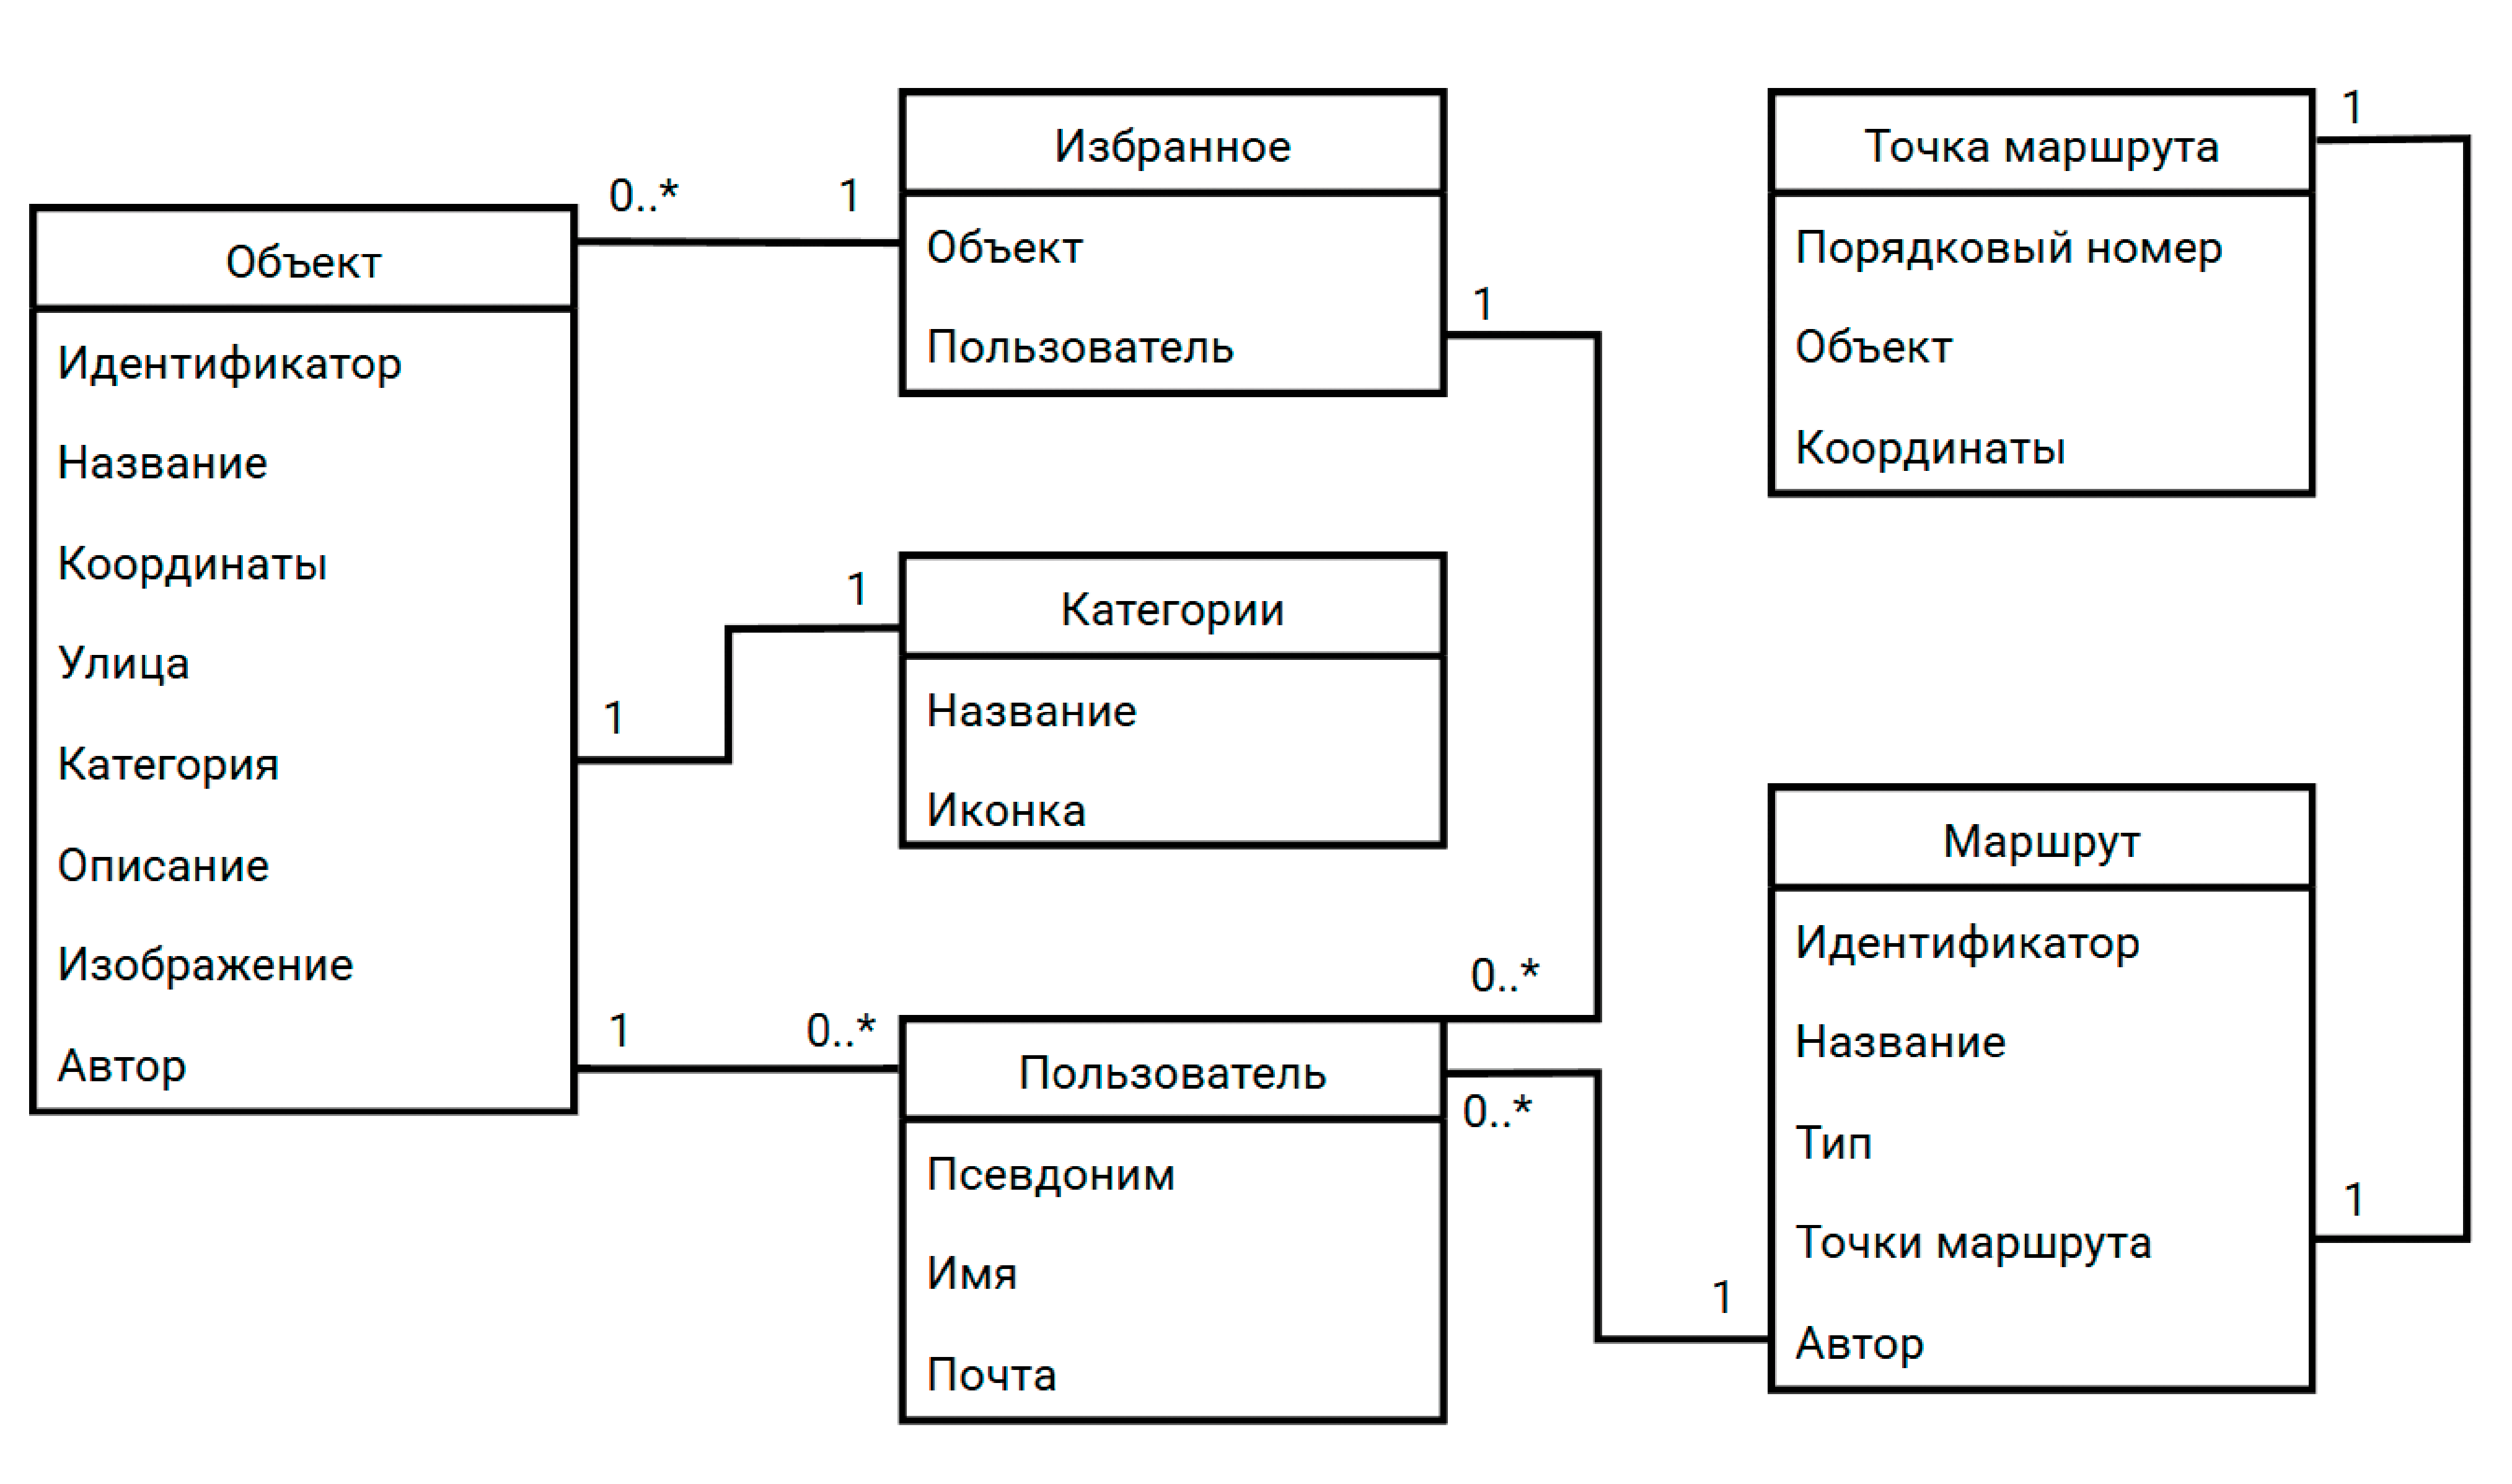
\includegraphics[width=1\linewidth]{comp}}
	\caption{Концептуальная модель данных}
	\label{comp:image}
\end{figure}

Вводимая информация:

Фильтрация объектов:
\begin{itemize}
	\item категория объекта (музеи, памятники, природные, религиозные и т. д.);
	\item уровень доступности (например, объекты с удобной парковкой, для людей с ОВЗ);
	\item расстояние от текущего местоположения.
\end{itemize}

Маршруты:
\begin{itemize}
	\item точка начала маршрута (может быть выбрана вручную или определена автоматически по геолокации);
	\item конечная и промежуточные точки (выбор из списка объектов или с карты);
	\item тип маршрута (пеший, автомобильный).
\end{itemize}

От внешних источников:
\begin{itemize}
	\item геолокация пользователя (через HTML5 API)\cite{b5};
	\item данные о достопримечательностях — из локальной базы или стороннего API;
	\item ответы от картографического сервиса (маршрутные данные).
\end{itemize}

Выводимая информация:

На главной и карте:
\begin{itemize}
	\item список доступных туристических объектов с краткой информацией\cite{b6} (название, категория, краткое описание);
	\item отображение объектов на карте (кастомные маркеры с всплывающими балунами);
	\item выделение объектов по фильтрам и поисковым запросам;
	\item визуальное отображение маршрута на карте с указанием начала, конца и промежуточных точек;
	\item подсказки/уведомления о текущем состоянии маршрута или выборе точек.
\end{itemize}

В балуне объекта:
\begin{itemize}
	\item название объекта;
	\item фотография или иконка;
	\item краткое описание;
	\item кнопки.
\end{itemize}

В панели маршрута:
\begin{itemize}
	\item адреса и названия всех точек маршрута;
	\item общая длина маршрута и ориентировочное время в пути;
	\item возможность изменения порядка точек;
	\item кнопка "Оптимизировать маршрут".
\end{itemize}

\subsubsection{Функциональные требования к программной системе}

Разрабатываемое веб-приложение должно обладать определённым набором функциональных возможностей, ориентированных на конечного пользователя — туриста. Основная задача системы — обеспечить удобный доступ к информации о туристических объектах Курской области и упростить процесс построения индивидуальных маршрутов\cite{b7}.

Основной функционал приложения:
\begin{enumerate}
	\item Отображение туристических объектов на карте.
	\item Возможность фильтрации объектов по категориям.
	\item Просмотр информации о выбранном объекте.
	\item Формирование персонального маршрута.
	\item Добавление точек маршрута вручную из списка или карты.
	\item Поддержка промежуточных точек и автоматическая прокладка оптимального пути.
	\item Выбор типа маршрута (пеший, автомобильный и др.).
	\item Автоматическое определение начальной точки (геолокация пользователя).
	\item Возможность редактирования порядка следования точек (перетаскивание, удаление).
	\item Возможность добавления/удаления объектов или маршрутов в избранное.
	\item Просмотр списка избранных точек на отдельной вкладке.
	\item Получение текущего местоположения пользователя с разрешения.
	\item Визуальное сопровождение движения по маршруту.
\end{enumerate}

На рисунке ~\ref{templ:image} в виде диаграммы прецедентов представлены функции, доступные всем пользователям.

На рисунке ~\ref{templauto:image} представлены дополнительные функции для авторизованных пользователей.

\begin{figure}[ht]
	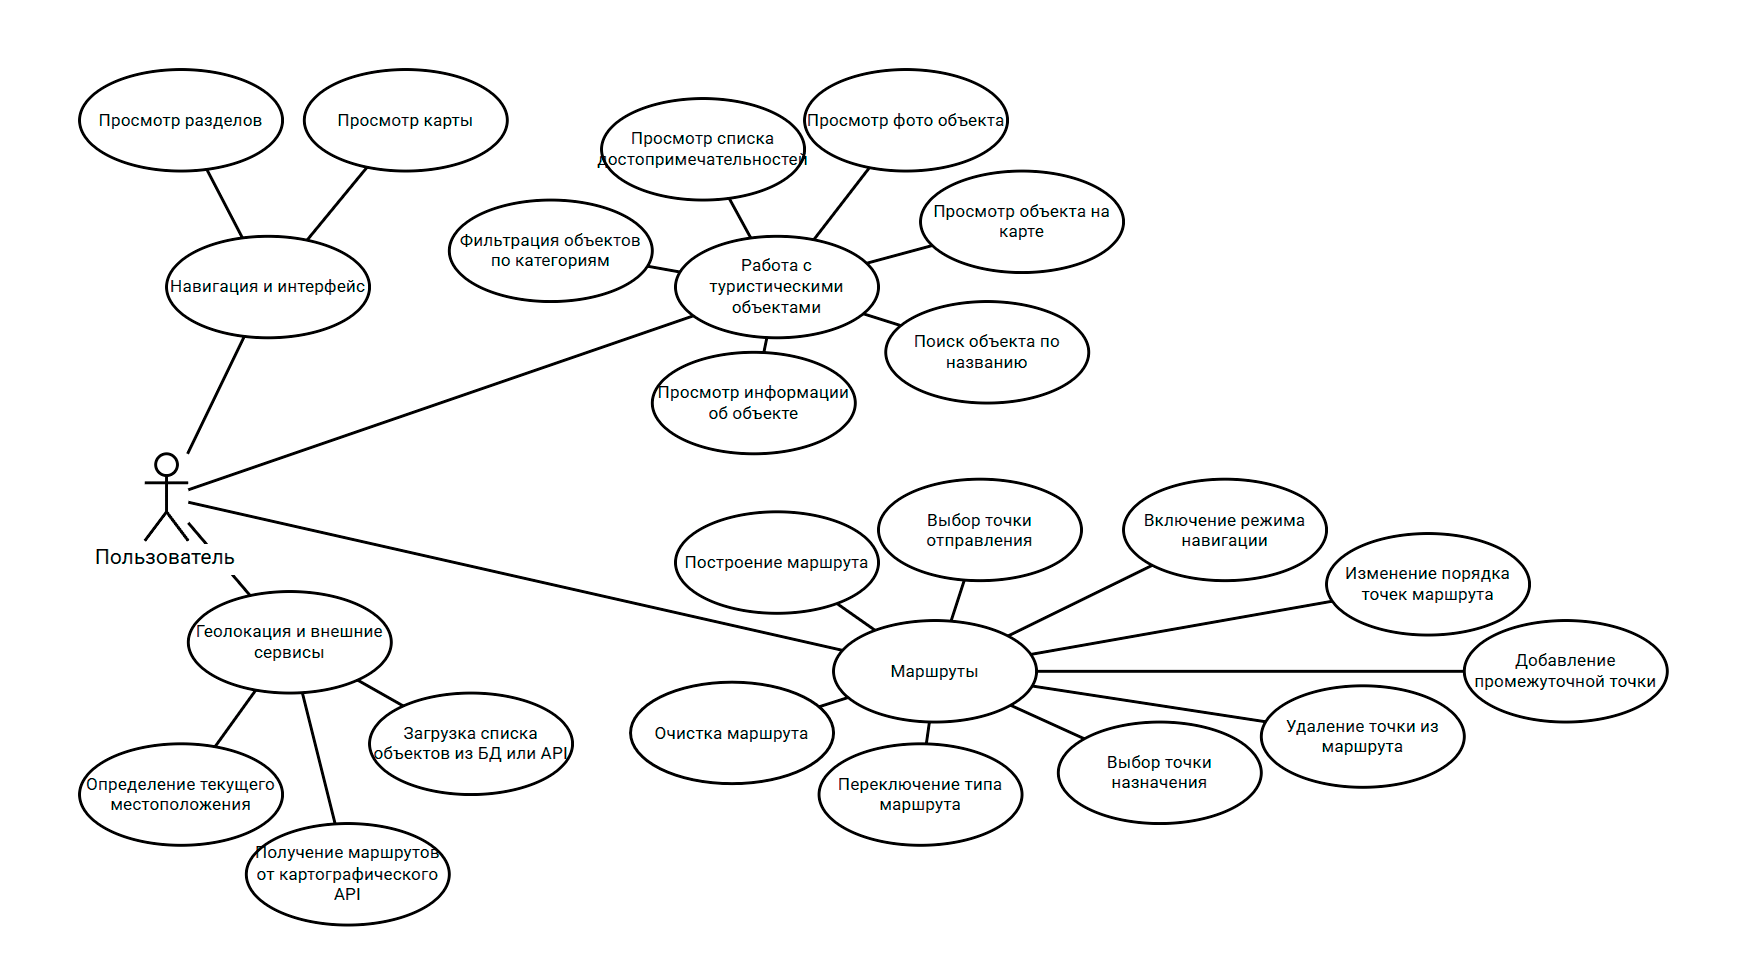
\includegraphics[width=1\linewidth]{templ}
	\caption{Диаграмма прецедентов}
	\label{templ:image}
\end{figure}

\vspace{+100mm}
\begin{figure}[ht]
	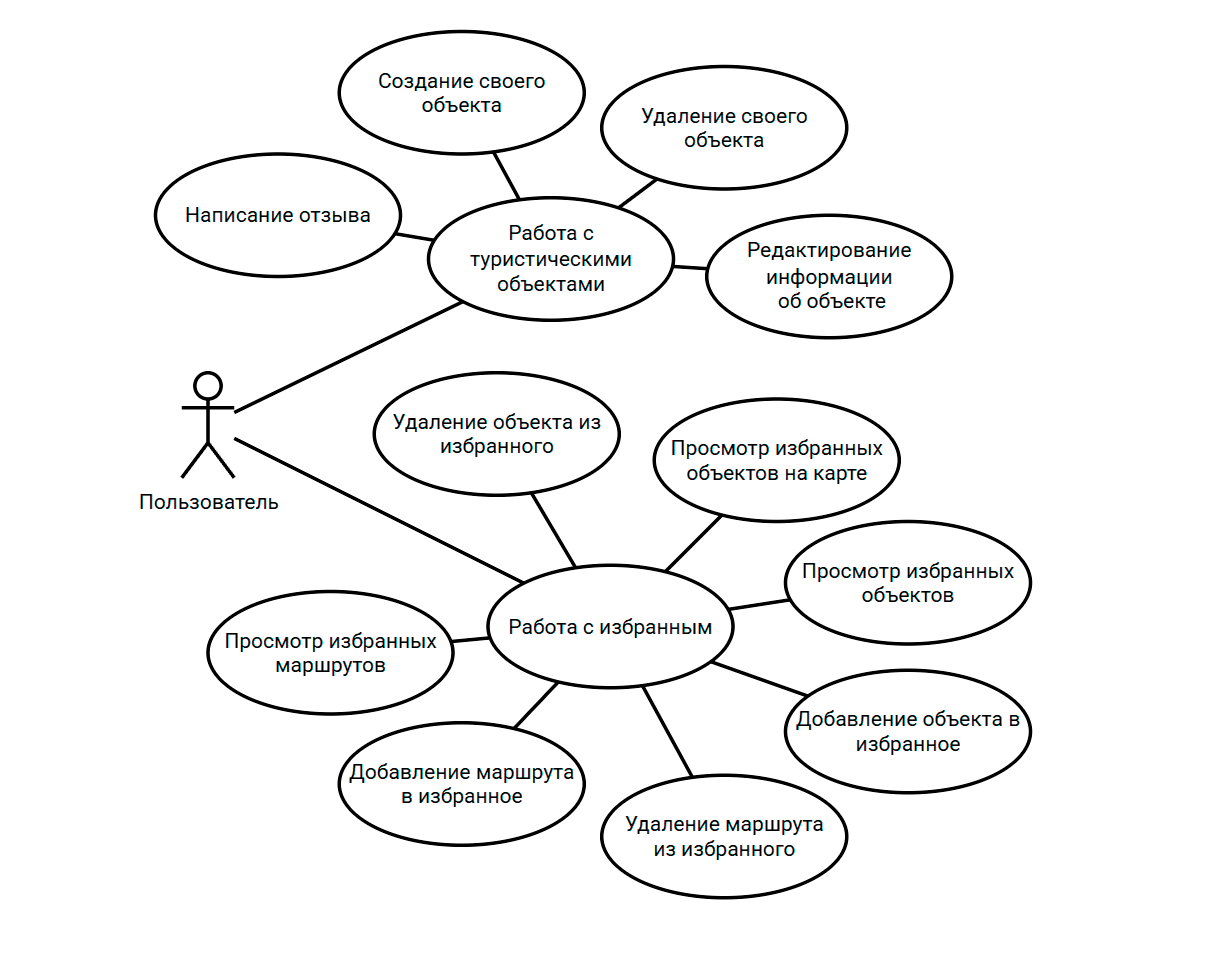
\includegraphics[width=1\linewidth]{templauto}
	\caption{Диаграмма прецедентов для авторизованного пользователя}
	\label{templauto:image}
\end{figure}

\subsubsection{Моделирование вариантов использования}
\paragraph{Вариант использования «Построение маршрута между туристическими объектами»}

Основной исполнитель: Пользователь

Заинтересованные лица и их требования:

Пользователь: хочет быстро построить удобный маршрут между выбранными достопримечательностями.

Система: должна обработать маршрут с учётом географических координат.

Предусловие: Пользователь выбрал как минимум две точки на карте.

Постусловие: Маршрут успешно построен и отображён на карте.

Основной успешный сценарий:
\begin{enumerate}
	\item Пользователь выбирает начальную и конечную точки.
	\item При необходимости добавляет промежуточные точки.
	\item Устанавливает тип маршрута (пеший или автомобильный).
	\item Система запрашивает маршрут у внешнего API.
	\item Построенный маршрут отображается на карте с указанием всех точек.
\end{enumerate}

\paragraph{Вариант использования «Фильтрация туристических объектов по категории»}

Основной исполнитель: Пользователь

Заинтересованные лица и их требования:

Пользователь: хочет отобразить только определённый тип объектов (например, музеи).

Система: обязана быстро применить фильтр и обновить карту.

Предусловие: Пользователь находится на странице карты.

Постусловие: На карте и в списке отображаются только объекты выбранной категории.

Основной успешный сценарий:
\begin{enumerate}
	\item Пользователь открывает панель фильтров.
	\item Отмечает нужные категории (одну или несколько).
	\item Система скрывает неактуальные объекты и обновляет видимость.
	\item Пользователь видит только интересующие его объекты.
\end{enumerate}

\paragraph{Вариант использования «Добавление объекта в избранное»}

Основной исполнитель: Авторизованный пользователь

Заинтересованные лица и их требования:

Пользователь: хочет сохранить интересные места для повторного просмотра.

Система: обязана привязать объект к конкретному пользователю.

Предусловие: Пользователь авторизован и открыл карточку объекта.

Постусловие: Объект сохранён в избранном пользователя.

Основной успешный сценарий:
\begin{enumerate}
	\item Пользователь открывает балун объекта.
	\item Нажимает кнопку "Добавить в избранное".
	\item Система отправляет данные на сервер.
	\item Сервер сохраняет связь между пользователем и объектом.
	\item Пользователь получает подтверждение об успешном добавлении.
\end{enumerate}

\paragraph{Вариант использования «Поиск объекта по ключевому слову»}

Основной исполнитель: Пользователь

Заинтересованные лица и их требования:

Пользователь: хочет быстро найти конкретную достопримечательность по названию.

Система: обязана предоставить релевантные результаты.

Предусловие: Пользователь находится на карте или в списке объектов.

Постусловие: Пользователь видит подходящие объекты на карте и/или в списке.

Основной успешный сценарий:
\begin{enumerate}
	\item Пользователь вводит ключевое слово в поисковую строку.
	\item Система фильтрует объекты, соответствующие запросу.
	\item Отображаются подходящие результаты.
	\item Пользователь может кликнуть по объекту для получения информации.
\end{enumerate}

\paragraph{Вариант использования «Определение текущего местоположения пользователя»}

Основной исполнитель: Пользователь

Заинтересованные лица и их требования:

Пользователь: хочет увидеть своё текущее местоположение на карте.

Система: обязана корректно запросить и отобразить координаты.

Предусловие: Пользователь дал разрешение на доступ к геолокации.

Постусловие: На карте отображается текущее местоположение пользователя.

Основной успешный сценарий:
\begin{enumerate}
	\item Пользователь нажимает кнопку "Отображать местоположение".
	\item Браузер запрашивает разрешение на доступ к геолокации.
	\item Пользователь разрешает.
	\item Система получает координаты и отображает метку на карте.
	\item Центр карты сдвигается на позицию пользователя.
\end{enumerate}

\paragraph{Вариант использования «Сохранение маршрута в личный кабинет»}

Основной исполнитель: Авторизованный пользователь

Заинтересованные лица и их требования:

Пользователь: хочет сохранить построенный маршрут для дальнейшего использования.

Система: должна обеспечить хранение маршрутов с возможностью последующего редактирования.

Предусловие: Пользователь авторизован и построил маршрут.

Постусловие: Маршрут сохранён в базе данных и доступен в профиле пользователя.

Основной успешный сценарий:
\begin{enumerate}
	\item Пользователь строит маршрут.
	\item Нажимает кнопку "Сохранить маршрут".
	\item Вводит название маршрута.
	\item Система отправляет маршрут на сервер.
	\item Сервер сохраняет маршрут, возвращает подтверждение.
	\item Пользователь видит сохранённый маршрут в личном кабинете.
\end{enumerate}

\paragraph{Вариант использования «Просмотр информации о достопримечательности»}

Основной исполнитель: Пользователь

Заинтересованные лица и их требования:

Пользователь: хочет узнать подробную информацию о конкретной точке интереса.

Администратор контента: ожидает, что пользователи получают корректные и актуальные сведения.

Предусловие: Пользователь нажал на объект на карте.

Постусловие: Открыта подробная карточка объекта с текстом, фото и ссылками.

Основной успешный сценарий:
\begin{enumerate}
	\item Пользователь кликает по маркеру на карте.
	\item Система отображает всплывающее окно (балун).
	\item Пользователь переходит к подробной карточке объекта.
	\item В карточке отображаются: название, описание, фото, категория, адрес, часы работы и др.
\end{enumerate}

\paragraph{Вариант использования «Сброс маршрута»}

Основной исполнитель: Пользователь

Заинтересованные лица и их требования:

Пользователь: хочет очистить текущие настройки, чтобы начать с чистого листа.

Система: должна корректно сбросить все активные параметры без сбоев.

Предусловие: Активен фильтр категорий или построен маршрут.

Постусловие: На карте отображаются все объекты, маршрут удалён.

Основной успешный сценарий:
\begin{enumerate}
	\item Пользователь закрывает панель настройки маршрута.
	\item Система удаляет маршрут с карты.
	\item Отображаются все объекты по умолчанию.
	\item Пользователь может начать новый поиск.
\end{enumerate}

\paragraph{Вариант использования «Перемещение точек маршрута вручную»}

Основной исполнитель: Пользователь

Заинтересованные лица и их требования:

Пользователь: хочет настроить порядок прохождения точек.

Система: должна позволить интерактивное изменение порядка точек.

Предусловие: Построен маршрут с несколькими точками.

Постусловие: Новый порядок точек сохранён, маршрут перестроен.

Основной успешный сценарий:
\begin{enumerate}
	\item Пользователь переходит к редактированию маршрута.
	\item Перетаскивает точки в нужном порядке.
	\item Система перестраивает маршрут.
	\item Новый маршрут отображается на карте.
\end{enumerate}

\paragraph{Вариант использования «Просмотр избранных объектов на карте»}

Основной исполнитель: Авторизованный пользователь

Заинтересованные лица и их требования:

Пользователь: хочет быстро отобразить все сохранённые объекты на карте.

Система: должна отобразить только объекты, находящиеся в избранном.

Предусловие: У пользователя есть добавленные в избранное объекты.

Постусловие: На карте отображаются маркеры только для избранных точек.

Основной успешный сценарий:
\begin{enumerate}
	\item Пользователь открывает раздел "Избранное".
	\item Нажимает кнопку "Показать на карте".
	\item Система запрашивает список избранных объектов.
	\item На карте появляются только эти точки.
	\item Карта центрируется на области с избранными.
\end{enumerate}

\paragraph{Вариант использования «Выбор типа маршрута»}

Основной исполнитель: Пользователь

Заинтересованные лица и их требования:

Пользователь: хочет выбрать наиболее удобный способ передвижения.

Система: должна перестроить маршрут с учётом выбранного типа.

Предусловие: Построен маршрут или выбраны точки.

Постусловие: На карте отображается актуальный маршрут соответствующего типа.

Основной успешный сценарий:
\begin{enumerate}
	\item Пользователь строит маршрут или выбирает точки.
	\item В интерфейсе выбирает тип маршрута (пеший или автомобильный).
	\item Система отправляет запрос в API с параметром типа маршрута.
	\item Полученный маршрут обновляется на карте.
	\item Пользователь получает маршрут, подходящий под выбранный режим.
\end{enumerate}

\paragraph{Вариант использования «Авторизация пользователя»}

Основной исполнитель: Пользователь

Заинтересованные лица и их требования:

Пользователь: хочет получить доступ к персональным функциям — избранному, сохранённым маршрутам.

Система: должна обеспечить безопасный вход и защиту данных.

Предусловие: Пользователь находится на сайте и не авторизован.

Постусловие: Пользователь авторизован и получает доступ к личным данным.

Основной успешный сценарий:
\begin{enumerate}
	\item Пользователь открывает форму авторизации.
	\item Вводит логин и пароль.
	\item Система проверяет данные и выдаёт токен.
	\item Открывается интерфейс с доступом к личному кабинету.
	\item Пользователь может работать с избранным и маршрутами.
\end{enumerate}

\paragraph{Вариант использования «Получение пошаговых инструкций к маршруту»}

Основной исполнитель: Пользователь

Заинтересованные лица и их требования:

Пользователь: хочет получить подробные указания по движению.

Система: должна предоставить навигационные шаги, основанные на маршруте.

Предусловие: Построен маршрут.

Постусловие: Пользователь видит текстовые инструкции по маршруту.

Основной успешный сценарий:
\begin{enumerate}
	\item Пользователь строит маршрут.
	\item Нажимает кнопку "Показать подробности".
	\item Система запрашивает информацию у картографического API.
	\item Отображается список шагов (поворотов, расстояний, ориентиров).
	\item Пользователь может следовать инструкции во время путешествия.
\end{enumerate}

\paragraph{Вариант использования «Просмотр подробной статистики о маршруте»}

Основной исполнитель: Пользователь

Заинтересованные лица и их требования:

Пользователь: хочет оценить длину, продолжительность, количество объектов на маршруте.

Система: должна проанализировать маршрут и отобразить метрики.

Предусловие: Маршрут построен.

Постусловие: Отображается статистика маршрута.

Основной успешный сценарий:
\begin{enumerate}
	\item Пользователь строит маршрут.
	\item Открывает вкладку с информацией.
	\item Система вычисляет: общее расстояние, количество точек, примерное время в пути.
	\item Отображает результаты в удобном формате.
	\item Пользователь принимает решение о корректировке или сохранении маршрута.
\end{enumerate}

\paragraph{Вариант использования «Оставление отзыва о туристическом объекте»}

Основной исполнитель: Авторизованный пользователь

Заинтересованные лица и их требования:

Пользователь: хочет поделиться впечатлениями о достопримечательности.

Администратор: стремится собирать обратную связь и отображать рейтинги.

Предусловие: Пользователь авторизован и посетил страницу объекта.

Постусловие: Отзыв сохранён и отображается в карточке объекта.

Основной успешный сценарий:
\begin{enumerate}
	\item Пользователь переходит на страницу объекта.
	\item Нажимает "Оставить отзыв".
	\item Заполняет форму с текстом и рейтингом.
	\item Система сохраняет отзыв в базу данных.
	\item Отзыв отображается другим пользователям.
\end{enumerate}

\paragraph{Вариант использования «Загрузка пользовательского объекта на карту»}

Основной исполнитель: Авторизованный пользователь

Заинтересованные лица и их требования:

Пользователь: хочет добавить малоизвестное или новое туристическое место.

Администратор: требует предварительной модерации перед публикацией.

Предусловие: Пользователь авторизован.

Постусловие: Объект добавлен в систему и ожидает модерации.

Основной успешный сценарий:
\begin{enumerate}
	\item Пользователь нажимает "Добавить объект".
	\item Заполняет форму с координатами, описанием, фото.
	\item Отправляет заявку.
	\item Система сохраняет данные и уведомляет модератора.
	\item После одобрения объект становится видимым другим пользователям.
\end{enumerate}

\paragraph{Вариант использования «Получение рекомендаций по маршрутам»}

Основной исполнитель: Пользователь

Заинтересованные лица и их требования:

Пользователь: хочет быстро получить готовые маршруты по своим интересам.

Система: должна учитывать предпочтения и текущие условия (время, погоду).

Предусловие: Пользователь указал интересы и параметры маршрута.

Постусловие: Отображаются подходящие готовые маршруты.

Основной успешный сценарий:
\begin{enumerate}
	\item Пользователь открывает раздел "Рекомендации".
	\item Выбирает интересующие категории и желаемую длительность.
	\item Система анализирует возможные маршруты.
	\item Показывает список наиболее подходящих.
	\item Пользователь выбирает и открывает один из маршрутов на карте.
\end{enumerate}

\paragraph{Вариант использования «Построение кольцевого маршрута»}

Основной исполнитель: Пользователь

Заинтересованные лица и их требования:

Пользователь: хочет маршрут, начинающийся и заканчивающийся в одной точке.

Система: должна правильно обработать алгоритм кольцевого построения.

Предусловие: Задана стартовая точка и фильтр интересов.

Постусловие: Отображается кольцевой маршрут на карте.

Основной успешный сценарий:
\begin{enumerate}
	\item Пользователь выбирает "Кольцевой маршрут".
	\item Вводит начальную точку и интересующие категории.
	\item Указывает допустимую длину/время маршрута.
	\item Система формирует кольцевой маршрут по заданным параметрам.
	\item Пользователь получает визуализацию маршрута и может начать навигацию.
\end{enumerate}

\paragraph{Вариант использования «Удаление точки маршрута»}

Основной исполнитель: Пользователь

Заинтересованные лица и их требования:

Пользователь: хочет исключить ненужную точку из маршрута.

Система: должна корректно пересчитать маршрут.

Предусловие: У пользователя открыт маршрут с несколькими точками.

Постусловие: Точка удалена, маршрут перестроен.

Основной успешный сценарий:
\begin{enumerate}
	\item Пользователь открывает список точек маршрута.
	\item Нажимает иконку удаления рядом с нужной точкой.
	\item Система удаляет точку из списка.
	\item Выполняется пересчёт маршрута.
	\item Новый маршрут отображается на карте. навигацию.
\end{enumerate}

\paragraph{Вариант использования «Оптимизация порядка точек маршрута по времени и расстоянию»}

Основной исполнитель: Пользователь

Заинтересованные лица и их требования:

Пользователь: хочет сэкономить время в пути, оптимизируя маршрут.

Система: должна автоматически пересчитать маршрут с наименьшими затратами по времени/расстоянию.

Предусловие: У пользователя уже создан маршрут с несколькими точками.

Постусловие: Система перестроила маршрут, изменив порядок точек для оптимального прохождения.

Основной успешный сценарий:
\begin{enumerate}
	\item Пользователь открывает сохранённый или текущий маршрут.
	\item Нажимает кнопку «Оптимизировать маршрут».
	\item Система анализирует возможные перестановки точек.
	\item Выполняется выбор наилучшего варианта с учётом расстояния и/или времени.
	\item Отображается обновлённый маршрут, пользователь может его сохранить или начать навигацию.
\end{enumerate}

\subsubsection{Требования к пользовательскому интерфейсу}

Интерфейс разрабатываемого веб-приложения должен быть визуально лёгким и адаптированным под широкую аудиторию\cite{b8} — от молодёжи до пожилых людей, путешествующих по Курской области. Основное внимание уделяется удобству взаимодействия, минимизации числа действий для выполнения ключевых операций, а также визуальной согласованности всех элементов.

Основными компонентами\cite{b9} интерфейса являются:
\begin{enumerate}
	\item Интерактивная карта региона, на которой отображаются туристические объекты. Карта  занимает центральное место в интерфейсе, так как с ней связано основное взаимодействие пользователя — поиск интересных мест, добавление точек маршрута и просмотр информации о достопримечательностях. Все элементы управления, связанные с картой, должны располагаться так, чтобы не перекрывать её значимую часть, при этом оставаться легко доступными.
	\item Панель фильтрации объектов. Она позволяет пользователю выбирать категории достопримечательностей, такие как музеи, архитектурные памятники, природные объекты и т. д.
	\item Форма построения маршрута. Она представляет собой всплывающее окно с полями «откуда», «куда» и возможностью добавления промежуточных точек.
	\item Карточка объекта. Она открывается при клике по метке на карте и в ней отображаются основная информация (название, фотография, описание), а также кнопки действий: добавление в маршрут, добавление в избранное, получение подробностей.
	\item Личный кабинет. В нем пользователь может просматривать сохранённые маршруты и избранные объекты.
\end{enumerate}

Интерфейс реализован на русском языке. Так же присутствует возможность реализации английской версии (в перспективе).

\subsubsection{Нефункциональный требования к программной системе}
\paragraph{Требования к надёжности}

Для обеспечения корректной и безопасной работы веб-приложения необходимо предусмотреть комплекс технических и организационных мер\cite{b10}, направленных на защиту пользовательских данных, устойчивость системы к ошибкам, сбоям и потенциальным угрозам со стороны злоумышленников.

Надёжность предполагает стабильную работу приложения в условиях стандартной пользовательской нагрузки, а также корректное поведение при возникновении нештатных ситуаций.

В рамках данного проекта под надёжностью понимается следующее:
\begin{enumerate}
	\item Обработка ошибок.	Все потенциальные ошибки (например, недоступность карты, сбои подключения к API, ошибки загрузки данных) должны обрабатываться с выводом понятного уведомления для пользователя без прекращения работы интерфейса.
	\item Валидация данных.	Все вводимые или получаемые извне данные должны проходить многоуровневую проверку на клиентской и серверной сторонах, что исключает возможность ошибок в логике или отображении.
	\item Резервирование критических элементов.	При использовании внешних API (например, картографических) рекомендуется реализовать fallback-механизмы или локальное кеширование часто используемых данных.
	\item Логирование. Серверная часть должна вести журнал событий (ошибок, действий пользователя, обращений к API) с целью оперативной диагностики и предотвращения сбоев.
\end{enumerate}

\paragraph{Требования к безопасности}

Безопасность данных пользователей, включая маршруты, избранное и потенциальную информацию о местоположении, является ключевым требованием. Для защиты информации применяются следующие меры:
\begin{enumerate}
	\item Шифрование трафика. Вся передача данных между клиентом и сервером должна осуществляться по протоколу HTTPS с использованием SSL/TLS-сертификатов.
	\item Контроль доступа. Регистрация и вход должны выполняться с защитой от подбора паролей (ограничение попыток, капча). Должны осуществляться хеширование паролей в базе данных (с применением алгоритмов bcrypt или Argon2) и защита пользовательских маршрутов и данных от несанкционированного доступа (привязка к сессии или токену).
	\item Защита от распространённых атак. 
	
	XSS (межсайтовый скриптинг): фильтрация HTML-содержимого в пользовательском вводе.
	
	CSRF (межсайтовая подделка запроса): защита форм с помощью токенов.
	
	SQL-инъекции: использование подготовленных запросов и ORM.
	
	CORS: настройка политик кросс-доменных запросов с ограничением доверенных источников.
\end{enumerate}

\paragraph{Требования к программной и аппаратной среде}

Для корректной работы и стабильного функционирования веб-приложения по отображению туристических объектов Курской области с функцией маршрутизации требуется соблюдение определённых условий по программной и аппаратной среде. Ниже приведены минимальные и рекомендуемые параметры для клиентской и серверной сторон.

Программные требования:

Клиентская часть (устройство пользователя):
\begin{itemize}
	\item операционные системы: Windows 10+, macOS 11+, Android 8.0+, iOS 13+;
	\item браузеры (актуальные версии): Google Chrome, Mozilla Firefox, Safari, Microsoft Edge;
	\item поддержка JavaScript и включённые cookie обязательны.
\end{itemize}

Серверная часть (хостинг или VPS):
\begin{itemize}
	\item операционная система: Ubuntu Server 20.04+ / Debian 11+ / CentOS 8+;
	\item веб-сервер: Apache (с поддержкой HTTPS);
	\item язык серверной логики: PHP (v8+);
	\item база данных: MySQL 8.0+;
	\item API и внешние сервисы: Яндекс.Карты API\cite{b11}.
\end{itemize}

Аппаратные требования:

Клиентское устройство:
\begin{itemize}
	\item процессор: двухъядерный от 1.5 ГГц;
	\item оперативная память: от 2 ГБ;
	\item разрешение экрана: от 1280×720.
\end{itemize}

Сервер:

Минимальные характеристики для пилотной версии:
\begin{itemize}
	\item CPU: 2 vCPU;
	\item RAM: 2–4 ГБ;
	\item SSD: от 20 ГБ;
	\item канал: не менее 100 Мбит/с.
\end{itemize}

Рекомендуемые характеристики для масштабируемой версии:
\begin{itemize}
	\item CPU: 4 vCPU и выше;
	\item RAM: 8 ГБ и выше;
	\item SSD: 40+ ГБ с возможностью масштабирования;
	\item резервное копирование данных раз в сутки.
\end{itemize}

\subsection{Требования к оформлению документации}

Разработка программной документации и программного изделия должна производиться согласно ГОСТ 19.102-77 и ГОСТ 34.601-90. Единая система программной документации.

Программная документация включает в себя:
\begin{enumerate}
	\item Анализ предметной области.
	\item Техническое задание.
	\item Технический проект.
	\item Рабочий проект.
\end{enumerate}

\section{Технический проект}
\subsection{Общая характеристика организации решения задачи}

В рамках решения задачи цифровизации туристической инфраструктуры региона была разработана концепция веб-приложения, ориентированного на широкую аудиторию — как местных жителей, так и туристов. Основной целью проекта стало создание удобной цифровой среды, позволяющей пользователю оперативно получать информацию о достопримечательностях, прокладывать маршруты и формировать персонализированные планы посещения.

Организация решения строится на модульном подходе\cite{b12}, при котором система разбивается на взаимосвязанные, но относительно независимые компоненты: модуль работы с картой, система фильтрации и поиска объектов, маршрутный модуль, интерфейс взаимодействия с пользователем, а также серверная логика, обеспечивающая хранение и обработку данных. Такое разделение упрощает поддержку и масштабирование проекта, позволяя в будущем дополнять его новыми возможностями без необходимости полной переработки архитектуры.

Веб-приложение функционирует в клиент-серверной модели\cite{b13}. Клиентская часть обеспечивает визуализацию данных, управление маршрутом и взаимодействие с картой, а серверная часть отвечает за хранение пользовательской информации, логирование действий, выдачу данных о туристических объектах, а также обработку маршрутов. Обмен между клиентом и сервером реализуется через REST API с использованием формата JSON, что обеспечивает гибкость и универсальность взаимодействия.

Информационное наполнение веб-приложения формируется из предварительно структурированных данных о достопримечательностях региона. Каждая точка интереса включает в себя географические координаты, категорию, краткое описание, изображения, а также дополнительные атрибуты, позволяющие фильтровать объекты по предпочтениям пользователя. Данные хранятся в базе, доступ к которой осуществляется с учётом требований безопасности и производительности.

\subsection{Обоснование выбора технологии проектирования}

Выбор технологий для реализации веб-приложения, посвящённого цифровой навигации по туристическим объектам региона, основывался на совокупности факторов: масштаб проекта, тип данных (в том числе геолокационных), необходимость интерактивного интерфейса и перспектива последующего расширения функционала. Особое внимание уделялось поддержке адаптивности, производительности и удобству взаимодействия с картографическими сервисами.

\subsubsection{Описание используемых технологий и языков программирования}

В процессе разработки web-сайта используются программные средства и языки программирования. Каждое программное средство и каждый язык программирования применяется для круга задач, при решении которых они необходимы.

\subsubsection{Язык разметки HTML}

HTML (HyperText Markup Language) — это стандартный язык разметки\cite{b19}, используемый для создания структуры веб-страниц. Он задаёт расположение и тип элементов интерфейса: заголовков, абзацев, кнопок, форм, списков и других компонентов. В рамках данного проекта HTML используется для:
\begin{itemize}
	\item определения компоновки интерфейса веб-приложения (например, блок карты, меню фильтров, карточки объектов);
	\item разметки форм маршрута, поиска и фильтрации точек интереса;
	\item обеспечения семантики, что повышает доступность и SEO-оптимизацию проекта;
	\item интеграции с JavaScript и стилями (CSS) — через идентификаторы, классы и атрибуты.
\end{itemize}

Благодаря чистой и логичной HTML-разметке упрощается последующее стилизование и взаимодействие с элементами через скрипты.

\subsubsection{Язык стилей CSS}

CSS используется для визуального оформления элементов, определения расположения блоков, выбора шрифтов, цветов и адаптации интерфейса под различные устройства. В проекте применяются:
\begin{itemize}
	\item анимации и визуальные эффекты для плавного появления элементов, наведения на кнопки и взаимодействия с маршрутом на карте;
	\item стилизация форм (полей ввода, выпадающих списков), карточек достопримечательностей, балунов карты и навигационных элементов.
\end{itemize}

CSS играет ключевую роль в восприятии системы конечным пользователем, обеспечивая привлекательность и удобство интерфейса.

\subsubsection{Язык программирования JavaScript}

JavaScript\cite{b18} — это язык программирования, который используется для добавления интерактивности на веб-страницах. Он позволяет обрабатывать действия пользователя, изменять элементы интерфейса без перезагрузки страницы и взаимодействовать с сервером. В проекте он используется для:
\begin{itemize}
	\item реализации фильтрации объектов в реальном времени без перезагрузки страницы;
	\item динамического добавления, удаления и сортировки точек маршрута;
	\item обработки кликов по карте, открытия балунов, взаимодействия с API Яндекс.Карт;
	\item обновления интерфейса в ответ на действия пользователя (например, отображение построенного маршрута, переключение категорий, переход между вкладками);
	\item отправки запросов к серверу и получения данных (API);
	\item управления состоянием интерфейса (например, сохранение списка избранного или выбранного типа маршрута).
\end{itemize}

JavaScript позволяет превратить статичную HTML-разметку в полноценное интерактивное приложение.

\subsubsection{Язык программирования PHP}

PHP — это язык серверной логики, работающий на стороне сервера. Он отвечает за обработку пользовательских запросов, взаимодействие с базой данных, управление сессиями и генерацию динамического HTML. Основные задачи PHP в рамках проекта:
\begin{itemize}
	\item формирование API-эндпоинтов для получения информации о точках интереса, маршрутах, пользователях;
	\item обработка входящих запросов: фильтрация, валидация, авторизация;
	\item хранение, обновление и удаление данных в базе;
	\item обеспечение безопасности;
	\item регистрация и авторизация пользователей, управление сессиями.
\end{itemize}

PHP, благодаря своей простоте и зрелой экосистеме, позволяет реализовать устойчивую и надёжную серверную часть с широкими возможностями по расширению.

\subsubsection{API Яндекс.Карт}

Яндекс.Карты API — это программный интерфейс, предоставляемый Яндексом для работы с их картографическим сервисом. Позволяет отображать интерактивные карты, добавлять метки, строить маршруты, использовать геолокацию и геокодинг.

Картографическое API Яндекс.Карт является ключевым компонентом проекта, обеспечивая визуальное отображение туристических объектов и построение маршрутов. Основные его функции в приложении:
\begin{itemize}
	\item отображение карты региона — с возможностью приближения, переключения слоёв и центрирования;
	\item добавление кастомных меток — каждая достопримечательность отображается своей иконкой, имеет всплывающий балун с описанием и кнопками действий;
	\item построение маршрутов — между произвольным количеством точек, включая начальную, конечную и промежуточные;
	\item кластеризация точек — при большом количестве объектов на карте они группируются в кластеры, упрощая восприятие;
	\item фильтрация и управление слоями — отображение только выбранных категорий (музеи, архитектурные объекты, природные и др.);
	\item интерактивность — пользователь может кликать по карте, добавлять точки маршрута, просматривать подробную информацию.
\end{itemize}

Использование Яндекс.Карт оправдано не только их функциональностью, но и точной локализацией и высокой детализацией регионов России, включая Курскую область.

\subsection{Архитектура программной системы}

Пользователь через браузер (клиентскую часть) отправляет запрос на построение маршрута. Этот запрос обрабатывается сервером Nginx и перенаправляется на PHP-приложение, которое обращается к базе данных\cite{b14} для получения информации об объектах, после чего строит маршрут с помощью API Яндекс.Карт. Готовый результат отправляется обратно пользователю в виде визуализации на карте и текстовых подсказок.

Программная система состоит из следующих компонентов:
\begin{enumerate}
	\item  Клиентская часть (Frontend). В основе клиентской части лежит набор веб-технологий, включая HTML, CSS и JavaScript. Эти технологии формируют пользовательский интерфейс, обеспечивающий визуальное взаимодействие с системой. HTML используется для структурирования содержимого страниц, CSS — для оформления и адаптации интерфейса под различные устройства, а JavaScript обеспечивает интерактивность. Например, действия пользователя, такие как выбор категории достопримечательностей или построение маршрута, обрабатываются с помощью JavaScript, который динамически обновляет содержимое без необходимости полной перезагрузки страницы. Отображение карты и точек на ней реализовано через подключение JavaScript-библиотеки Яндекс.Карт, позволяющей накладывать пользовательские метки, маршруты и настраивать поведение интерфейса карты.
	\item Промежуточный сервер (Web Server). Между клиентом и сервером располагается прокси-сервер, который выполняет роль маршрутизатора. Он принимает все входящие HTTP-запросы, обрабатывает их на начальном уровне (например, применяет HTTPS-шифрование, фильтрует запросы и кеширует часто используемые ресурсы), а затем перенаправляет их на сервер приложений. Такая прослойка значительно повышает производительность и безопасность системы.
	\item Сервер приложений (Backend). На серверной стороне работает программная логика, написанная на PHP. Здесь происходит основная обработка данных. Когда пользователь, например, строит маршрут между двумя туристическими объектами, PHP-скрипты получают данные о начальной и конечной точке, выполняют проверку и, при необходимости, обращаются к API Яндекс.Карт для получения оптимального маршрута. PHP также взаимодействует с базой данных, в которой хранятся сведения обо всех достопримечательностях, пользователях, отзывах, избранных местах и сохранённых маршрутах.
	\item Внешние API. Важным элементом архитектуры является использование внешних API. Центральное место здесь занимает API Яндекс.Карт, который обеспечивает не только отображение карты, но и функционал геокодирования (преобразование адресов в координаты), построение маршрутов с различными параметрами (пешком, на машине, на общественном транспорте) и вывод вспомогательных подсказок. Благодаря этому API веб-приложение получает возможность предоставить пользователю высокоинтерактивную карту с широкими возможностями.
\end{enumerate}

На рисунке \ref{data:image} представлена архитектура программной системы.

\begin{figure}[ht]
	\center{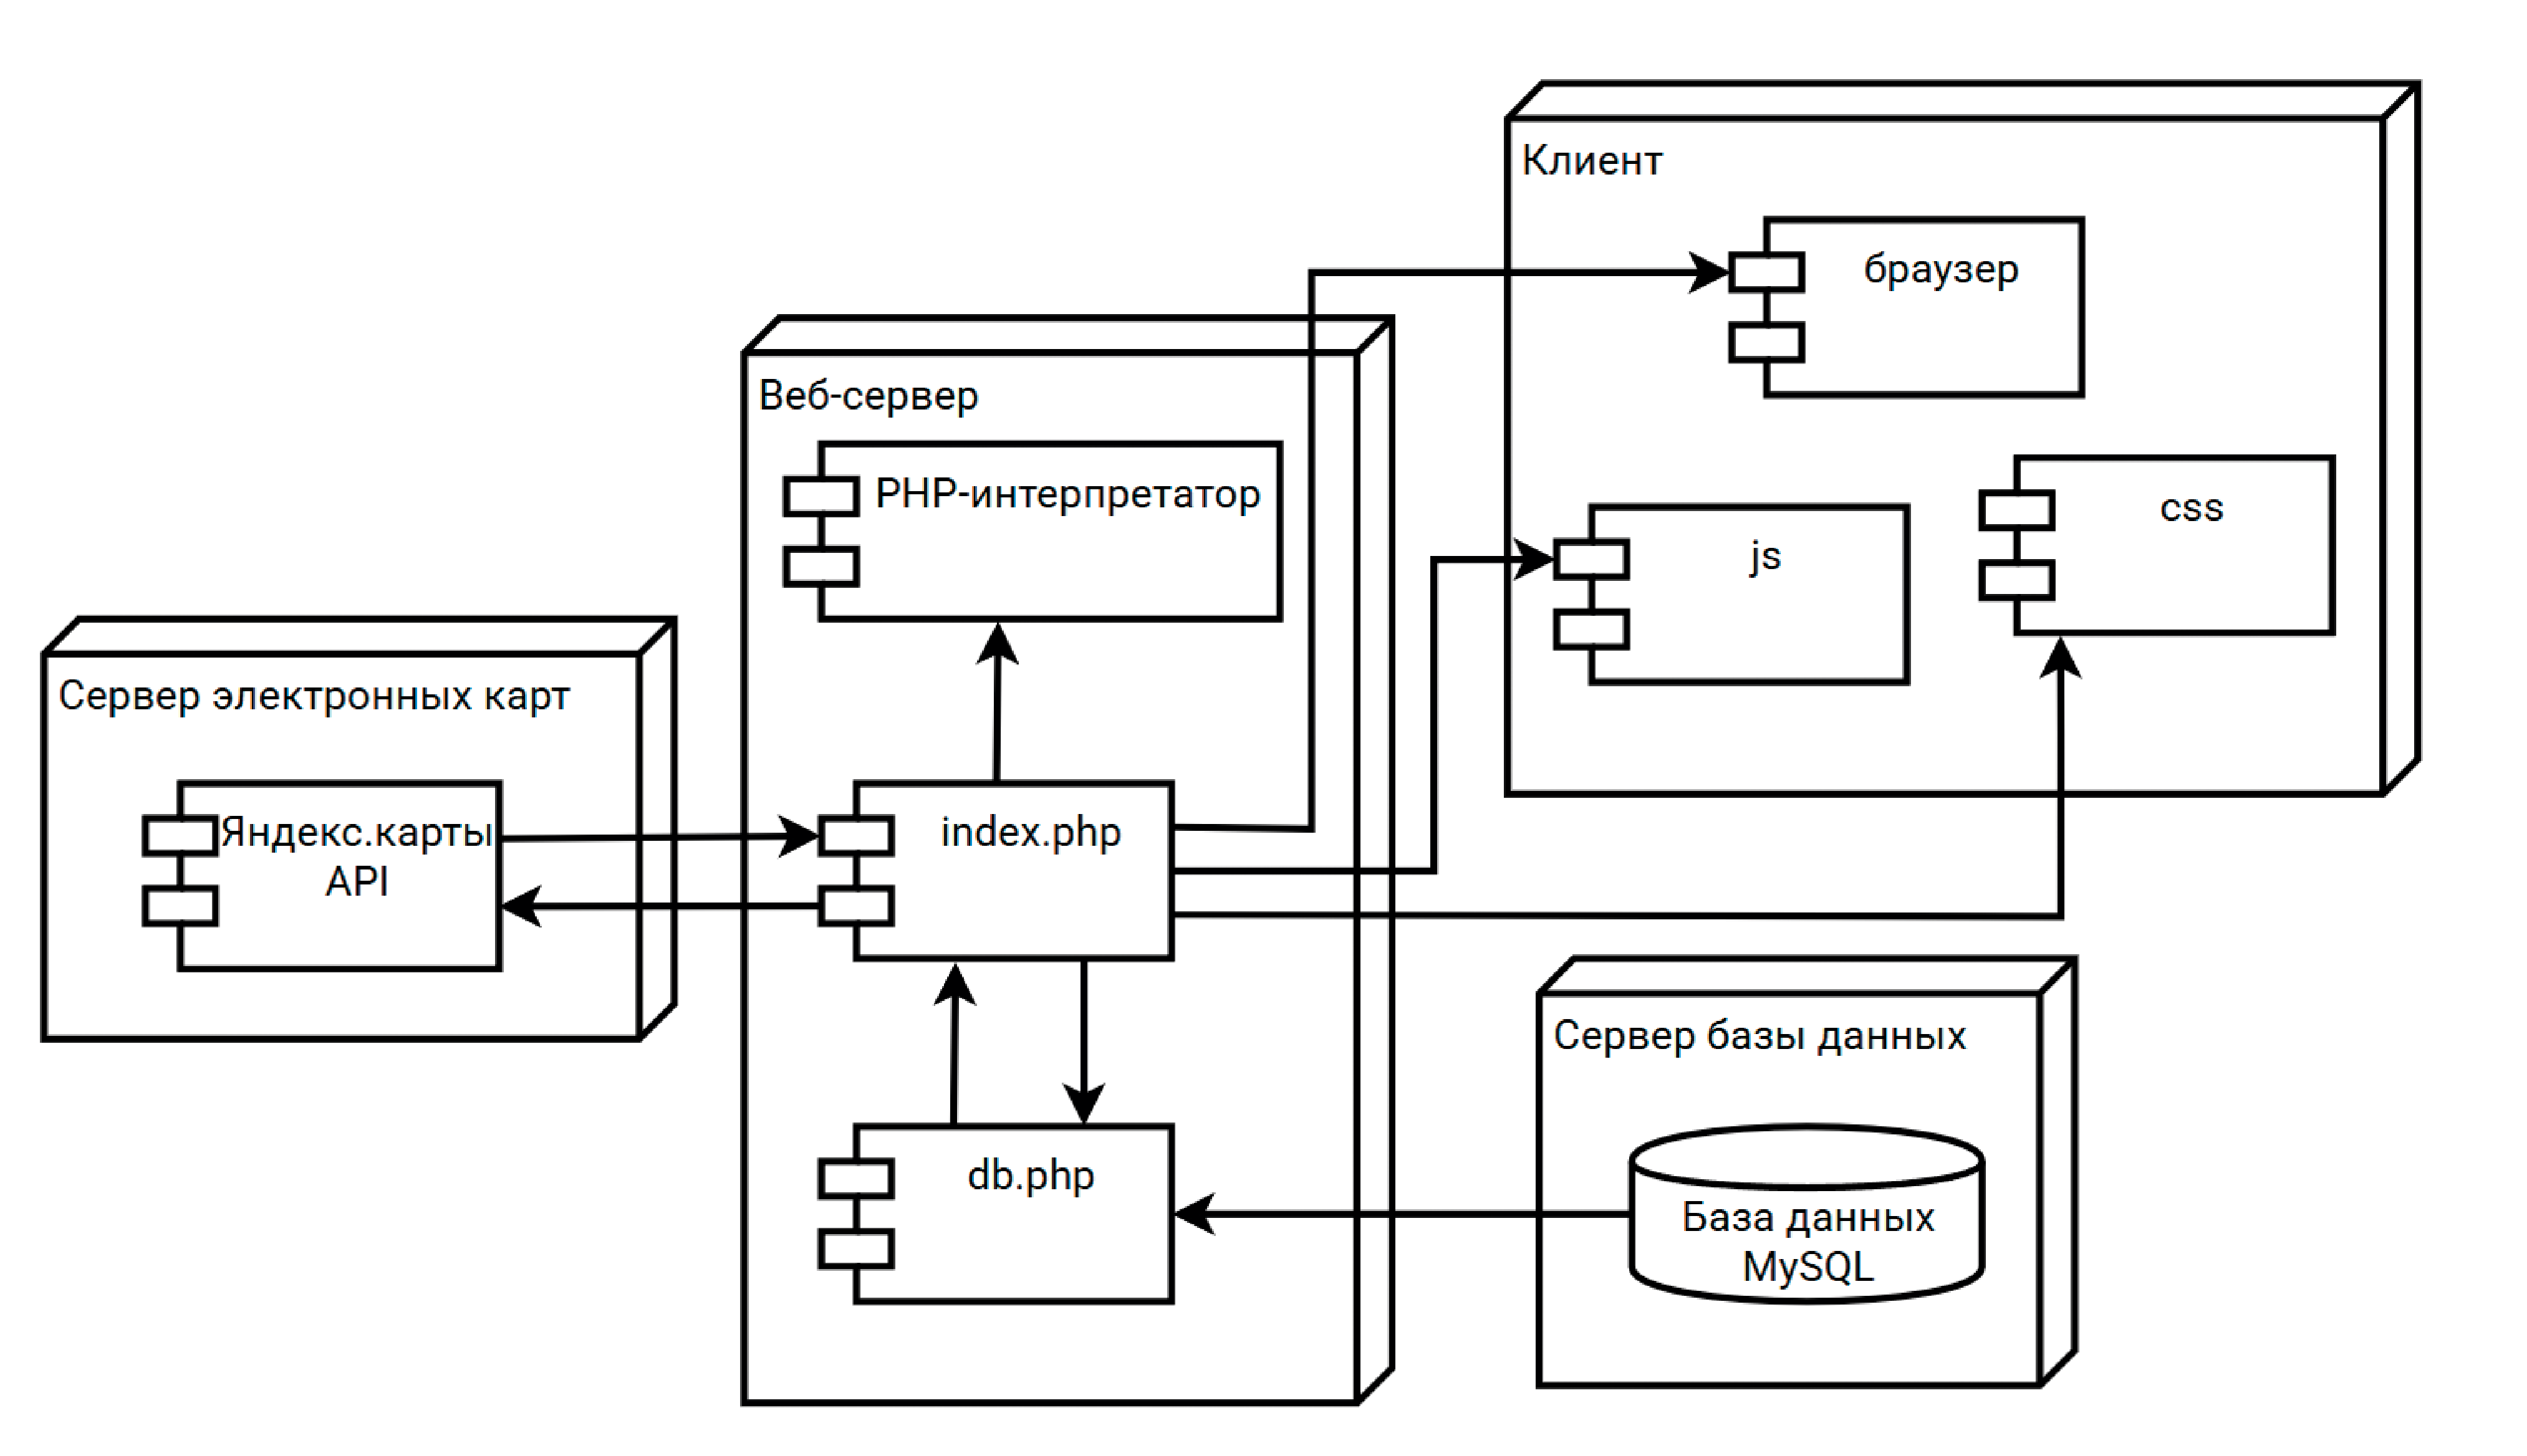
\includegraphics[width=1\linewidth]{data}}
	\caption{Архитектура программной системы}
	\label{data:image}
\end{figure}

\subsection{Построение маршрутов и интеграция с API Яндекс.Карт}

Одна из ключевых задач разрабатываемого веб-приложения — обеспечение функционала построения маршрутов между выбранными туристическими объектами. В отличие от стандартных навигационных систем, где путь прокладывается между двумя точками, пользователь данного приложения может создавать маршруты произвольной сложности с промежуточными остановками, сортировать порядок следования точек и выбирать предпочтительный тип передвижения. Для реализации этой функциональности используется API Яндекс.Карт — мощный инструмент, предоставляющий средства работы с геоданными, маршрутизацией и визуализацией картографической информации.

Особенности построения маршрутов. 
Построение маршрута начинается с выбора пользователем начальной точки, которая по умолчанию может быть определена автоматически через функцию геолокации. Затем пользователь добавляет любые доступные на карте объекты, при этом порядок следования можно изменять вручную, а также добавлять или удалять точки в любой момент.

На техническом уровне маршрут строится через объект ymaps.multiRouter.MultiRoute, который позволяет задать массив точек и параметры маршрута. Библиотека Яндекс.Карт производит расчет маршрута на стороне сервера, возвращая данные о длине пути, времени в пути и последовательности сегментов. Пользователь видит не только визуальное отображение маршрута на карте, но и текстовые инструкции (при активации пошагового режима), а также общую сводку по расстоянию и продолжительности.

Типы маршрутов. 
Приложение поддерживает выбор типа маршрута: пеший, автомобильный и общественный транспорт. Это реализуется через передачу параметра "type" в объект маршрута, что влияет на алгоритм расчета пути и предлагаемые траектории.

Работа с промежуточными точками. 
Одной из особенностей является возможность добавления промежуточных точек маршрута в произвольной последовательности. Пользователь может строить не только прямой путь «из точки A в точку B», но и составлять полноценный маршрут, охватывающий несколько достопримечательностей. Для этого формируется массив routePoints, содержащий все выбранные координаты. При необходимости маршрут можно реорганизовать — переставив точки местами, что приводит к пересчёту пути без перезагрузки карты.

Интерактивность и обновление. 
Маршрут пересчитывается автоматически при каждом изменении списка точек или их порядка. Это обеспечивает интерактивность и гибкость взаимодействия\cite{b15}. Пользователь может видеть, как меняется маршрут в реальном времени, что особенно важно при планировании маршрутов разной протяжённости и сложности. При этом используется минимальное количество ресурсов клиента, поскольку вычисления происходят на стороне Яндекса.

Визуализация и пользовательский интерфейс. 
Каждый маршрут сопровождается графическим отображением на карте с различными стилями оформления в зависимости от типа маршрута. Метки начальной, промежуточной и конечной точек выделяются визуально, а маршруты отображаются цветной линией. При наведении или клике пользователь может получить дополнительную информацию о точке или сегменте пути.

Таким образом, модуль маршрутизации является неотъемлемой частью веб-приложения и его основной пользовательской ценностью. Благодаря использованию API Яндекс.Карт удаётся добиться высокой точности расчётов, стабильной работы и масштабируемости, при этом интерфейс остаётся удобным даже для неподготовленного пользователя.

\subsection{Проект данных программной системы}

Разработка эффективной системы хранения и обработки информации требует чёткого проектирования структуры данных, отражающей как сущности предметной области, так и характер их взаимодействия. В данном случае речь идёт о цифровой платформе, отображающей туристические объекты региона, позволяющей пользователю формировать маршруты, оставлять отзывы и сохранять интересные места. Соответственно, проект данных опирается на ключевые сущности: объекты на карте, маршруты, пользователи, категории, отзывы и избранное. Все эти компоненты взаимосвязаны, и их модель должна обеспечивать целостность, логичность и возможность масштабирования.

Центральным элементом системы является туристический объект. Он представляет собой точку интереса, отображаемую на карте и содержащую базовую информацию: координаты, название, описание, привязку к определённой категории, а также опционально — изображения. Каждый такой объект может быть отображён на маршруте, добавлен в избранное и иметь прикреплённые отзывы.

Пользователи являются участниками системы с различным уровнем доступа. Для них предусматривается хранение учётной информации: адреса электронной почты, зашифрованного пароля, имени и роли в системе. Пользователь может быть как обычным посетителем, формирующим маршруты и просматривающим карту, так и администратором, получающим доступ к инструментам модерации. В базе данных с каждым пользователем связывается его история маршрутов и список избранных объектов.

Особое внимание уделяется маршрутам, которые пользователь может строить вручную. Структура маршрута должна быть гибкой, чтобы позволять добавление произвольного числа точек, определение порядка следования и выбор типа передвижения. Поэтому маршруты представлены двумя уровнями данных: заголовочной частью (название, тип маршрута) и набором точек маршрута. Каждая точка в маршруте включает координаты, название и, при наличии, связь с объектом из основного справочника. Дополнительно может храниться информация об адресе, полученная в процессе геокодирования, и флаг, указывающий на начальную точку.

Отдельно проектируется подсистема отзывов, позволяющая пользователям оставлять текстовые комментарии к объектам. Каждый отзыв содержит информацию об авторе, времени публикации, тексте сообщения и объекте, к которому он относится. Это позволяет в дальнейшем использовать отзывы для формирования пользовательского рейтинга, а также для отображения обратной связи в интерфейсе приложения.

Для организации и группировки объектов вводится система категорий. Каждая категория содержит идентификатор, название и визуальный признак (иконку), который используется при отображении на карте. Такая структура позволяет гибко фильтровать отображаемые точки и упрощает восприятие данных.

Существенную роль играет механизм избранного. Это логическая связь между пользователем и объектами, которые он отметил для последующего просмотра. Связь реализуется как отдельная сущность, позволяющая фиксировать не только факт добавления. Такая структура полезна при персонализации интерфейса или последующем анализе пользовательского поведения.

Вся модель данных строится с учётом реляционной логики и соблюдением принципов нормализации. Это позволяет обеспечить отсутствие дублирования информации, упрощает поддержку данных в актуальном состоянии и способствует стабильной работе при росте объёма пользователей и объектов.

Таким образом, проект данных представляет собой структурированную и логически выстроенную модель взаимодействующих сущностей, на которых основана работа веб-приложения. Он обеспечивает надёжную основу для хранения и обработки информации, поддерживает расширяемость проекта и отвечает требованиям удобства как для пользователя, так и для администратора системы.

Исходя из требований, можно выделить следующие основные сущности:

\begin{itemize}
	\item Пользователи
	\item Туристические объекты
	\item Категории объектов
	\item Избранное
	\item Маршруты
	\item Точки маршрута
	\item Отзывы
\end{itemize}

В состав сущности "<Пользователи"> можно включить атрибуты, представленные в таблице \ref{news:table}.

\begin{xltabular}{\textwidth}{|l|l|p{1.7cm}|X|}
	\caption{Атрибуты сущности "<Пользователи">\label{news:table}}\\ \hline
	\centrow Поле & \centrow Тип & \centrow Обяза\-тельное & \centrow Описание \\ \hline
	\thead{1} & \thead{2} & \centrow 3 & \centrow 4 \\ \hline
	\endfirsthead
	\continuecaption{Продолжение таблицы \ref{news:table}}
	\thead{1} & \thead{2} & \centrow 3 & \centrow 4 \\ \hline
	\finishhead
	id & Integer & true & Уникальный идентификатор пользователя \\ \hline 
	name & Varchar & true & Отображаемое имя пользователя \\ \hline 
	email & Varchar & true & Адрес электронной почты (уникальный) \\ \hline 
	password\_hash & Varchar & true & Хешированный пароль \\ \hline 
	role & Enum & true & Роль пользователя (например: user, admin)
	
\end{xltabular}

В состав сущности "<Туристические объекты"> можно включить атрибуты, представленные в таблице \ref{news:table1}.

\begin{xltabular}{\textwidth}{|l|l|p{1.7cm}|X|}
	\caption{Атрибуты  сущности "<Туристические объекты">\label{news:table1}}\\ \hline
	\centrow Поле & \centrow Тип & \centrow Обяза\-тельное & \centrow Описание \\ \hline
	\centrow 1 & \centrow 2 & \thead{3} & \centrow 4 \\ \hline
	\endfirsthead
	\continuecaption{Продолжение таблицы \ref{news:table1}}
	\centrow 1 & \centrow 2 & \thead{3} & \centrow 4 \\ \hline
	\finishhead
	id & Integer & true & Уникальный идентификатор туристического объекта \\ \hline 
	name & Varchar & true & Название объекта \\ \hline 
	description & Text & false & Краткое описание объекта \\ \hline  
	latitude & Float & true & Географическая широта объекта \\ \hline   
	longitude & Float & true & Географическая долгота объекта \\ \hline  
	category\_id & Integer & true & Идентификатор категории, к которой принадлежит объект\\ \hline  
	image\_url & Varchar & false & Ссылка на изображение объекта \\ \hline 
	created\_by & Integer & false & ID пользователя, добавившего объект \\ \hline 
	is\_active & Boolean & true & Флаг отображения объекта на карте
	
\end{xltabular}

В состав сущности "<Категории объектов"> можно включить атрибуты, представленные в таблице \ref{news:table2}.

\begin{xltabular}{\textwidth}{|l|l|p{1.7cm}|X|}
	\caption{Атрибуты  сущности "<Категории объектов">\label{news:table2}}\\ \hline
	\centrow Поле & \centrow Тип & \centrow Обяза\-тельное & \centrow Описание \\ \hline
	\centrow 1 & \centrow 2 & \thead{3} & \centrow 4 \\ \hline
	\endfirsthead
	\continuecaption{Продолжение таблицы \ref{news:table2}}
	\centrow 1 & \centrow 2 & \thead{3} & \centrow 4 \\ \hline
	\finishhead
	id & Integer & true & Уникальный идентификатор категории \\ \hline 
	name & Varchar & true & Название категории (например, Музей, Природа) \\ \hline 
	icon & Varchar & false & Путь к иконке категории для отображения на карте
		
\end{xltabular}

В состав сущности "<Избранное"> можно включить атрибуты, представленные в таблице \ref{news:table3}.

\begin{xltabular}{\textwidth}{|l|l|p{1.7cm}|X|}
	\caption{Атрибуты  сущности "<Избранное">\label{news:table3}}\\ \hline
	\centrow Поле & \centrow Тип & \centrow Обяза\-тельное & \centrow Описание \\ \hline
	\centrow 1 & \centrow 2 & \thead{3} & \centrow 4 \\ \hline
	\endfirsthead
	\continuecaption{Продолжение таблицы \ref{news:table3}}
	\centrow 1 & \centrow 2 & \thead{3} & \centrow 4 \\ \hline
	\finishhead
	user\_id & Integer & true & ID пользователя, добавившего объект в избранное \\ \hline 
	point\_id & Integer & true & ID объекта, добавленного в избранное
	
\end{xltabular}

В состав сущности "<Маршруты"> можно включить атрибуты, представленные в таблице \ref{news:table4}.

\begin{xltabular}{\textwidth}{|l|l|p{1.7cm}|X|}
	\caption{Атрибуты  сущности "<Маршруты">\label{news:table4}}\\ \hline
	\centrow Поле & \centrow Тип & \centrow Обяза\-тельное & \centrow Описание \\ \hline
	\centrow 1 & \centrow 2 & \thead{3} & \centrow 4 \\ \hline
	\endfirsthead
	\continuecaption{Продолжение таблицы \ref{news:table4}}
	\centrow 1 & \centrow 2 & \thead{3} & \centrow 4 \\ \hline
	\finishhead
	id & Integer & true & Уникальный идентификатор маршрута \\ \hline 
	user\_id & Integer & true & ID пользователя, создавшего маршрут \\ \hline 
	name & Varchar & true & Название маршрута \\ \hline 
	type & Enum & true & Тип маршрута (например, пеший, автомобильный)
	 
\end{xltabular}

В состав сущности "<Точки маршрута"> можно включить атрибуты, представленные в таблице \ref{news:table5}.

\begin{xltabular}{\textwidth}{|l|l|p{1.7cm}|X|}
	\caption{Атрибуты  сущности "<Точки маршрута">\label{news:table5}}\\ \hline
	\centrow Поле & \centrow Тип & \centrow Обяза\-тельное & \centrow Описание \\ \hline
	\centrow 1 & \centrow 2 & \thead{3} & \centrow 4 \\ \hline
	\endfirsthead
	\continuecaption{Продолжение таблицы \ref{news:table5}}
	\centrow 1 & \centrow 2 & \thead{3} & \centrow 4 \\ \hline
	\finishhead
	id & Integer & true & Уникальный идентификатор точки маршрута \\ \hline 
	route\_id & Integer & true & ID маршрута, к которому принадлежит точка \\ \hline 
	point\_id & Integer & false & ID объекта (если точка — это объект карты) \\ \hline 
	latitude & Float & false & Широта точки (если она не связана с объектом) \\ \hline 
	longitude & Float & false & Долгота точки (если она не связана с объектом) \\ \hline 
	address & Varchar & false & Адрес точки (результат геокодирования) \\ \hline 
	order\_index & Integer & true & Порядковый номер точки в маршруте
	
\end{xltabular}

В состав сущности "<Отзывы"> можно включить атрибуты, представленные в таблице \ref{news:table6}.

\begin{xltabular}{\textwidth}{|l|l|p{1.7cm}|X|}
	\caption{Атрибуты  сущности "<Отзывы">\label{news:table6}}\\ \hline
	\centrow Поле & \centrow Тип & \centrow Обяза\-тельное & \centrow Описание \\ \hline
	\centrow 1 & \centrow 2 & \thead{3} & \centrow 4 \\ \hline
	\endfirsthead
	\continuecaption{Продолжение таблицы \ref{news:table6}}
	\centrow 1 & \centrow 2 & \thead{3} & \centrow 4 \\ \hline
	\finishhead
	id & Integer & true & Уникальный идентификатор отзыва \\ \hline 
	user\_id & Integer & true & ID пользователя, оставившего отзыв \\ \hline 
	point\_id & Integer & true & ID объекта, к которому относится отзыв \\ \hline 
	content & Text & true & Текстовое содержание отзыва 
	
\end{xltabular}

\subsection{Проектирование пользовательского интерфейса}

Создание удобного и визуально сбалансированного пользовательского интерфейса\cite{b16} является одной из ключевых задач при разработке веб-приложений, ориентированных на широкую аудиторию. В контексте проекта по цифровизации туристических объектов региона особую роль играет не только функциональность интерфейса, но и его способность направлять внимание пользователя, упрощать взаимодействие с интерактивной картой и быстро предоставлять доступ к основным действиям: фильтрации, маршрутизации, просмотру информации и управлению своим профилем.

Интерфейс спроектирован таким образом, чтобы пользователю было достаточно одного экрана для выполнения большинства операций — от навигации по карте до построения маршрута. Центром внимания в приложении служит карта, отображающая туристические объекты. Остальные элементы располагаются по периферии и не перекрывают рабочую область, а открываются по необходимости: например, боковые панели, выпадающие меню и модальные окна. Такой подход обеспечивает сохранение ориентации на карте и минимизирует визуальные помехи.

Проектирование интерфейса основано на модульной структуре. Каждый элемент системы, будь то фильтр категорий, форма построения маршрута или карточка объекта, разрабатывается как самостоятельный интерфейсный блок. Это упрощает как техническую реализацию (например, переиспользование компонентов), так и восприятие для пользователя, поскольку каждое действие логически отделено и выполняется в своей зоне.

Взаимодействие с пользователем начинается с загрузки карты, на которой по умолчанию отображаются все активные туристические объекты региона. Навигация осуществляется через элементы фильтрации, позволяющие мгновенно скрывать или показывать объекты определённых категорий. При наведении на метку пользователь получает краткую информацию об объекте во всплывающем балуне, а при клике — расширенную карточку с описанием, изображением и кнопками действий (добавить в маршрут, избранное, оставить отзыв).

Отдельное внимание уделено проектированию маршрутизатора — интерфейса для построения пользовательских маршрутов. В соответствующем окне пользователь указывает начальную и конечную точки, а также может добавлять промежуточные. Система автоматически прокладывает маршрут с помощью внешнего API\cite{b17} и отображает его на карте в реальном времени. Информация о маршруте, включая продолжительность и длину, отображается в отдельной панели. Особенность реализации заключается в возможности интерактивного редактирования порядка точек, что позволяет гибко настраивать путь.

Аутентификация пользователей реализуется через минималистичную форму входа и регистрации. После авторизации появляются дополнительные элементы интерфейса. Непрерывная работа сессии и визуальное подтверждение действий (например, уведомление о добавлении в избранное) создают ощущение целостности и контроля над процессом.

Визуальный стиль интерфейса стремится к простоте и функциональной чистоте. Используются нейтральные цвета фона, акцентные кнопки. Отступы и иконки подобраны так, чтобы элементы не сливались, но и не перегружали экран. Большинство компонентов адаптированы под мобильные устройства: меню сворачиваются, форма маршрута упрощается, карта масштабируется под маленькие экраны.

Особое внимание в процессе проектирования уделено доступности\cite{b20}. Все интерактивные элементы имеют контрастную визуализацию, поддерживают навигацию с клавиатуры, а всплывающие уведомления сопровождаются альтернативным текстом. Такой подход расширяет аудиторию и соответствует современным рекомендациям по доступному веб-дизайну.

На рисунке \ref{gr1:image} представлен макет основного окна веб-приложения. Он содержит следующие элементы:

\begin{enumerate}
	\item Карта.
	\item Панель управления("<Маршрут">, "<Фильтр">, "<Создание точки">, "<Авторизация">).
	\item Метка объекта на карте.
	\item Кнопка включения и выключения геолокации.
	\item Поиск по слову.
	\item Масштаб.
\end{enumerate}

\vspace{+40mm}
\begin{figure}[ht]
	\center{
\includegraphics[width=1\linewidth]{gr1}}
	\caption{Макет интерфейса}
	\label{gr1:image}
\end{figure}

На рисунке \ref{gr7:image} представлен макет формы "<Маршрут">. Ниже показаны следующие его элементы:

\begin{enumerate}
	\item Точка маршрута.
	\item Кнопка удаления точки из маршрута.
	\item Кнопка для добавления маршрута в избранное.
	\item Кнопки для переключения типа маршрута.
	\item Кнопка для оптимизации маршрута.
	\item Информация о длине и примерном времени маршрута.
	\item Кнопка включения и выключение подробным инструкций.
	\item Пошаговые инструкции.
	\item Кнопки закрытия формы без очистки маршрута.
	\item Кнопка закрытия формы и очистки маршрута.
\end{enumerate}

\begin{figure}[ht]
	\center{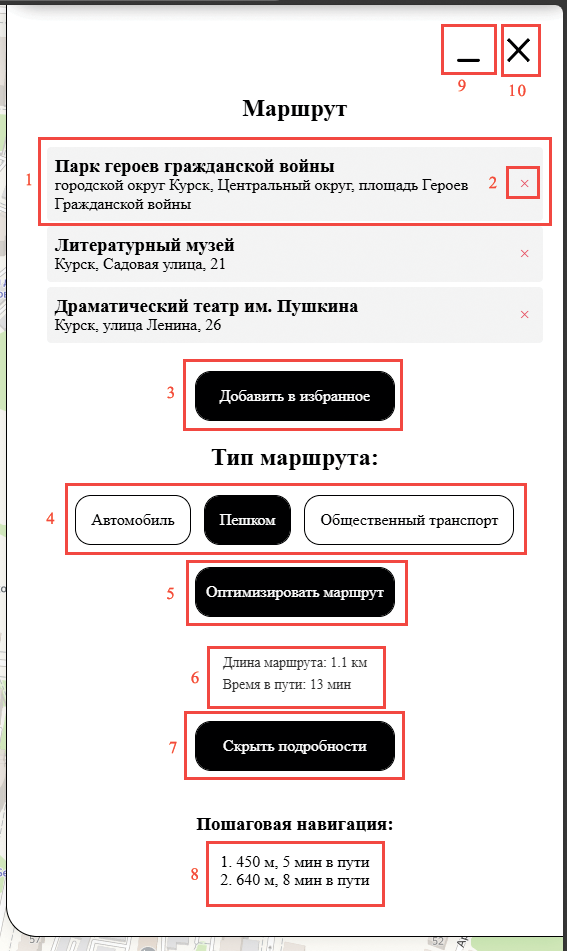
\includegraphics[width=0.5\linewidth]{gr7}}
	\caption{Макет интерфейса "<Маршрут">}
	\label{gr7:image}
\end{figure}

На рисунке \ref{gr4:image} представлен макет формы "<Фильтр">. Макет содержит следующие элементы:

\begin{enumerate}
	\item Кнопки закрытия формы.
	\item Флаги включения и выключения отображения типов объектов на карте.
\end{enumerate}

\vspace{+80mm}
\begin{figure}[ht]
	\center{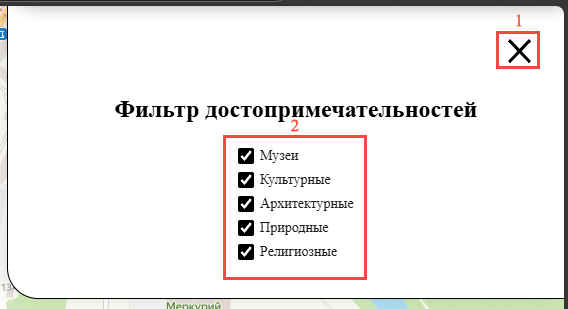
\includegraphics[width=1\linewidth]{gr4}}
	\caption{Макет интерфейса "<Фильтр">}
	\label{gr4:image}
\end{figure}

На рисунке \ref{gr5:image} представлен макет формы "<Создание точки">. Он содержит следующие элементы:

\begin{enumerate}
	\item Поле ввода названия.
	\item Адрес точки.
	\item Список для выбора категории.
	\item Кнопки подтверждения.
	\item Расположение метки на карте.
	\item Кнопка закрытия формы.
\end{enumerate}

\vspace{+80mm}
\begin{figure}[ht]
	\center{
\includegraphics[width=1\linewidth]{gr5}}
	\caption{Макет интерфейса "<Создание точки">}
	\label{gr5:image}
\end{figure}

На рисунке \ref{gr8:image} представлен макет формы "<Авторизация"> в случае, если пользователь еще не был зарегистрирован. Ниже показаны следующие его элементы:

\begin{enumerate}
	\item Поле ввода псевдонима.
	\item Поле ввода электронной почты.
	\item Поле ввода пароля.
	\item Поле подтверждения пароля.
	\item Кнопка подтверждения.
	\item Кнопка перехода в форму входа.
	\item Кнопка закрытия формы.
\end{enumerate}

\vspace{+40mm}
\begin{figure}[ht]
	\center{
\includegraphics[width=1\linewidth]{gr8}}
	\caption{Макет интерфейса "<Авторизация">. Пользователь регистрируется впервые.}
	\label{gr8:image}
\end{figure}

На рисунке \ref{gr9:image} представлен макет формы "<Авторизация"> в случае, когда пользователь вошел в личный кабинет. Макет содержит следующие элементы:

\begin{enumerate}
	\item Список избранных мест.
	\item Список избранных маршрутов.
	\item Избранное место.
	\item Кнопка удаления из избранного.
	\item Кнопка выхода из личного кабинета.
	\item Кнопка закрытия формы.
\end{enumerate}

\begin{figure}[ht]
	\center{
\includegraphics[width=1\linewidth]{gr9}}
	\caption{Макет интерфейса "<Авторизация">. Личный кабинет пользователя.}
	\label{gr9:image}
\end{figure}
\ifПрактика{}\else{
	\section{Рабочий проект}
\subsection{Спецификация компонентов программной системы}

Можно выделить следующий список классов и их методов, использованных при разработке web-приложения\cite{b25} (таблица \ref{class:rtable}).

\begin{xltabular}{\textwidth}{|p{4cm}|X|}
\caption{Описание классов, используемых в веб-приложении\label{class:rtable}}\\
\hline \centrow Название класса & \centrow Описание класса\\
\hline \centrow 1 & \centrow 2\\ \hline
\endfirsthead
\continuecaption{Продолжение таблицы \ref{class:rtable}}
\centrow 1 & \centrow 2\\ \hline
\finishhead
index.php & Основная веб-страница, отображающая интерактивную карту и элементы пользовательского интерфейса. Позволяет управлять фильтрами, маршрутами, добавлением объектов и аккаунтом. Подключает JavaScript-компоненты и карты Яндекса.\\
\hline add\_object.php & Обрабатывает отправку данных при добавлении новой точки. Сохраняет координаты, название, категорию и адрес в базу. Поддерживает модерацию.\\
\hline auth.php & Определяет текущий статус авторизации пользователя и возвращает результат в формате JSON.\\
\hline check\_favorite.php & Проверяет наличие определённого объекта в списке избранного пользователя. Возвращает булево значение в JSON.\\
\hline check-auth.php & Проверяет наличие активной пользовательской сессии. Используется для динамической загрузки элементов интерфейса в зависимости от статуса авторизации (например, отображение меню аккаунта). Возвращает ответ в формате JSON.\\
\hline data.php & Загружает данные о точках с учётом прав доступа. Отдаёт описание, изображения и категорию объектов.\\
\hline db.php & Содержит параметры подключения к базе данных и инициализирует PDO-соединение. Используется другими PHP-скриптами.\\
\hline delete\_route.php & Удаляет сохранённый маршрут из базы, предварительно проверяя авторизацию пользователя.\\
\hline functions.php & Набор вспомогательных функций для валидации данных форм, очистки ввода и отображения ошибок.\\
\hline get\_favorite\_\-points.php & Возвращает список точек, добавленных пользователем в избранное, включая координаты и названия.\\
\hline get\_favorite\_\-routes.php & Загружает маршруты из избранного, включая последовательность точек и тип маршрута.\\
\hline get\_point\_name.php & Определяет название объекта по его координатам. Применяется для генерации названий в маршрутах.\\
\hline get\_images.php & Загружает изображения, прикреплённые к определённой туристической точке. Возвращает массив ссылок на изображения, применяемый в карточке объекта и балуне.\\
\hline get\_reviews.php & Загружает все отзывы, связанные с конкретным объектом. Возвращает текст, авторов и даты.\\
\hline login.php & Осуществляет проверку введённого email и пароля. При успешной проверке инициирует сессию.\\
\hline logout.php & Завершает пользовательский сеанс, удаляя сессионные данные и перенаправляя на главную страницу.\\
\hline moderate.php & Интерфейс модерации для администраторов. Позволяет управлять статусом новых объектов, описаний и изображений.\\
\hline register.php & Регистрирует новых пользователей, проводит валидацию данных и сохраняет хешированный пароль.\\
\hline save\_object.php & Обрабатывает дополнительную информацию для объектов (описания, изображения). Поддерживает модерацию.\\
\hline save\_point.php & Добавляет или убирает точку из избранного. Возвращает результат действия.\\
\hline save\_route.php & Сохраняет маршрут в профиль пользователя: координаты точек, тип маршрута, название.\\
\hline send\_review.php & Добавляет отзыв к выбранному объекту. Проверяет авторизацию перед сохранением.\\
\hline addData.js & Отвечает за отправку данных при добавлении нового объекта. Проверяет авторизацию перед отправкой.\\
\hline addObject.js & Позволяет взаимодействовать с временной меткой на карте при добавлении объекта: перемещение, адрес.\\
\hline addObject\-Information.js & Управляет формой для добавления описания и изображений к существующему объекту.\\
\hline addObjectPicture.js & Реализует предпросмотр и удаление изображений перед отправкой.\\
\hline addReview.js & Обрабатывает отображение и отправку отзывов. Подгружает существующие отзывы с сервера.\\
\hline favoritePoint.js & Отвечает за добавление и удаление точек из избранного, а также обновление визуального состояния.\\
\hline Filter.js & Реализует фильтрацию точек на карте по выбранным категориям. Изменяет видимость меток.\\
\hline loadFavorites\-Points.js & Загружает избранные точки пользователя и отображает их на карте с возможностью удаления.\\
\hline loadFavorites\-Routes.js & Загружает маршруты из избранного и отображает их на карте. Обеспечивает удаление маршрутов.\\
\hline Location.js & Определяет текущие координаты пользователя через Geolocation API и отображает их на карте.\\
\hline openAccount\-Menu.js & Управляет открытием и скрытием меню аккаунта, включая вход, регистрацию и личный кабинет.\\
\hline openAddMenu.js & Отвечает за отображение меню добавления новых объектов на карту.\\
\hline openFilterMenu.js & Управляет отображением меню фильтрации объектов по категориям.\\
\hline openRegistration\-Menu.js & Отвечает за форму регистрации, обрабатывает валидацию и отображение ошибок.\\
\hline openRouteMenu.js & Отображает меню построения маршрутов, управления точками и сохранения.\\
\hline routeHandler.js & Основной модуль маршрутизации. Строит и обновляет маршруты, рассчитывает расстояние и длительность.\\
\hline openObjectInfor\-mationMenu.js & Отвечает за отображение панели редактирования информации об объекте. Активирует форму добавления описания и изображений, а также подгружает текущие данные, если они уже существуют.\\
\hline openSearchMenu.js & Отвечает за открытие и закрытие панели поиска. Обрабатывает ввод поискового запроса пользователем, фокусирует поле ввода и управляет визуальной активностью панели. Интегрирован с фильтрацией или подсказками.\\
\end{xltabular}

\subsubsection{Спецификация файла routeHandler.js}

В таблице \ref{class:rtable1} представлены функции файла favoritePoint.js.

\begin{xltabular}{\textwidth}{|p{5cm}|X|}
	\caption{Функции файла routeHandler.js\label{class:rtable1}}\\
	\hline \centrow Название функции & \centrow Описание функции\\
	\hline \centrow 1 & \centrow 2\\ \hline
	\endfirsthead
	\continuecaption{Продолжение таблицы \ref{class:rtable1}}
	\centrow 1 & \centrow 2\\ \hline
	\finishhead
	setMapInstance(map) & Сохраняет экземпляр карты в переменную mapInstance для использования в других частях приложения.\\
	\hline setupRouteTypeButtons() & Назначает обработчики кнопок выбора типа маршрута (пеший, авто и др.). Обновляет активное состояние и перерисовывает маршрут при необходимости.\\
	\hline optimizeRoute() & Выполняет простую оптимизацию порядка точек маршрута на основе жадного алгоритма ближайшей точки.\\
	\hline getDistance(coords1, coords2) & Вычисляет расстояние между двумя координатами по формуле haversine. Используется в оптимизации маршрута.\\
	\hline toRad(degrees) & Преобразует градусы в радианы для расчёта расстояния между координатами.\\
	\hline attachRouteButton\-Handler(coords, title) & Привязывает кнопку в балуне к добавлению точки в маршрут. Вызывает addRoutePoint.\\
	\hline addRoutePoint(coords, title) & Добавляет выбранную точку в маршрут. При первом добавлении определяет текущее местоположение как стартовую точку.\\
	\hline getPointNameFrom\-DB(coords, callback) & Выполняет fetch-запрос к серверу для получения названия точки по координатам.\\
	\hline drawCustomRoute() & Строит маршрут на карте с использованием API Яндекс.Карт. Отображает данные о длине и времени маршрута, обновляет интерфейс.\\
	\hline formatTime(minutes) & Форматирует время маршрута в удобный вид: часы и минуты.\\
	\hline openRouteMenu() & Показывает меню управления маршрутом, если оно скрыто.\\
	\hline updateRouteListUI() & Обновляет список точек маршрута в интерфейсе на основе текущего состояния массива routePoints.\\
	\hline enableRouteListSorting() & Включает возможность перетаскивания и изменения порядка точек в маршруте.\\
	\hline getAddressesForRoute\-Points() & Выполняет обратное геокодирование точек маршрута для отображения адресов.\\
	\hline setupResetButton() & Назначает обработчик на кнопку сброса маршрута. При нажатии очищает маршрут и интерфейс.\\
	\hline resetRoute() & Полностью удаляет текущий маршрут, очищает карту и связанные элементы интерфейса.\\
	\hline removeRoute\-Point(index) & Удаляет точку из маршрута по индексу и перерисовывает маршрут.\\
	\hline setupRouteModal\-Handlers() & Назначает обработчики модального окна сохранения маршрута: открыть, закрыть, подтвердить.\\
	\hline showRouteNameModal() & Проверяет авторизацию и минимальное количество точек. Если условия соблюдены — показывает модальное окно для ввода названия маршрута.\\
	\hline hideRouteNameModal() & Скрывает модальное окно сохранения маршрута.\\
	\hline saveFavoriteRouteWith\-Name() & Отправляет маршрут с названием на сервер для сохранения в избранное.\\
	\hline initInstructionsToggle() & Управляет видимостью блока пошаговых инструкций по маршруту. Назначает обработчик на кнопку переключения.\\
	\hline showNavigationInstruc\-tionsFromMulti\-Route(route) & Извлекает сегменты маршрута из API Яндекс.Карт и формирует HTML-блок с пошаговыми указаниями.\\
	\hline setPointsInstance(points) & Сохраняет список всех точек в переменную allPoints для последующего анализа.\\
	\hline getOptimalCircular\-RoutePoints() & Строит кольцевой маршрут вокруг временной метки с заданной длиной, выбирая ближайшие точки до достижения лимита.\\
	\hline setupCircularRoute() & Назначает обработчик на кнопку построения кольцевого маршрута. Запускает процесс выбора оптимальных точек.\\
\end{xltabular}

\subsubsection{Спецификация файла addObject.js}

В таблице \ref{class:rtable2} представлены функции файла addObject.js.

\begin{xltabular}{\textwidth}{|p{5cm}|X|}
	\caption{Функции файла addObject.js\label{class:rtable2}}\\
	\hline \centrow Название функции & \centrow Описание функции\\
	\hline \centrow 1 & \centrow 2\\ \hline
	\endfirsthead
	\continuecaption{Продолжение таблицы \ref{class:rtable2}}
	\centrow 1 & \centrow 2\\ \hline
	\finishhead
	addPlacemark(map) & Создаёт на карте временную метку в центре экрана, которая может быть перемещена пользователем. При перемещении обновляет поля с адресом и координатами. Также назначает обработчик для удаления метки и очистки полей при закрытии панели добавления. Использует геокодирование для получения текстового адреса.\\
	\hline updateAddressAnd\-Coordinates(coords) & Выполняет обратное геокодирование координат, получая адрес с помощью ymaps.geocode(). После получения адреса заполняет соответствующие поля формы: текстовый адрес и числовые значения широты и долготы. Используется для обновления данных при перемещении временной метки.\\
\end{xltabular}

\subsubsection{Спецификация файла addReview.js}

В таблице \ref{class:rtable3} представлены функции файла addReview.js.

\begin{xltabular}{\textwidth}{|p{6cm}|X|}
	\caption{Функции файла addReview.js\label{class:rtable3}}\\
	\hline \centrow Название функции & \centrow Описание функции\\
	\hline \centrow 1 & \centrow 2\\ \hline
	\endfirsthead
	\continuecaption{Продолжение таблицы \ref{class:rtable3}}
	\centrow 1 & \centrow 2\\ \hline
	\finishhead
	addReviewToList(review) & Добавляет переданный отзыв в начало списка на странице. Создаёт HTML-элемент <li>, форматирует дату отзыва и отображает его содержимое в пользовательском интерфейсе.\\
	\hline loadReviews(objectId) & Загружает отзывы с сервера по идентификатору объекта. Отображает список отзывов в интерфейсе или сообщение об отсутствии данных. В случае ошибки выводит сообщение о неудачной загрузке.\\
\end{xltabular}

\subsubsection{Спецификация файла favoritePoints.js}

В таблице \ref{class:rtable4} представлены функции файла favoritePoints.js.

\begin{xltabular}{\textwidth}{|p{5cm}|X|}
	\caption{Функции файла favoritePoints.js\label{class:rtable4}}\\
	\hline \centrow Название функции & \centrow Описание функции\\
	\hline \centrow 1 & \centrow 2\\ \hline
	\endfirsthead
	\continuecaption{Продолжение таблицы \ref{class:rtable4}}
	\centrow 1 & \centrow 2\\ \hline
	\finishhead
	attachFavoriteButton\-Handler(pointId) & Назначает обработчик на кнопку «добавить в избранное» в балуне объекта. При клике выполняет добавление точки и обновление визуального состояния.\\
	\hline addToFavorites(pointId) & Асинхронно проверяет авторизацию пользователя и отправляет запрос на добавление/удаление точки из избранного. Возвращает результат действия.\\
	\hline loadFavoritePoints() & Загружает с сервера текущий список избранных точек пользователя и вызывает их отображение.\\
	\hline renderFavorite\-Points(points) & Отрисовывает список избранных точек в интерфейсе. Назначает обработчики для перемещения к точке на карте и удаления из избранного.\\
	\hline removeFrom\-Favorites(pointId, element, point) & Удаляет точку из избранного, обновляет интерфейс, повторно открывает балун при необходимости и показывает сообщение, если список стал пустым.\\
	\hline reopenBalloonFor\-Point(point) & Повторно открывает балун объекта на карте, если он был закрыт после обновления состояния избранного.\\
	\hline updateFavoriteButton\-InBalloon(pointId, isFavorite) & Обновляет внешний вид кнопки «избранное» в балуне соответствующего объекта в зависимости от его текущего статуса.\\
	\hline focusPointOn\-Map(point) & Центрирует карту на координатах указанной точки и открывает её балун, если объект найден среди отображаемых.\\
\end{xltabular}

\subsubsection{Спецификация файла loadFavoritesRoutes.js}

В таблице \ref{class:rtable5} представлены функции файла loadFavoritesRoutes.js.

\begin{xltabular}{\textwidth}{|p{6cm}|X|}
	\caption{Функции файла loadFavoritesRoutes.js\label{class:rtable5}}\\
	\hline \centrow Название функции & \centrow Описание функции\\
	\hline \centrow 1 & \centrow 2\\ \hline
	\endfirsthead
	\continuecaption{Продолжение таблицы \ref{class:rtable5}}
	\centrow 1 & \centrow 2\\ \hline
	\finishhead
	loadFavoriteRoutes() & Загружает с сервера список маршрутов, сохранённых пользователем в избранное, и передаёт данные в функцию отрисовки.\\
	\hline renderFavorite\-Routes(routes) & Отображает полученные маршруты в интерфейсе. Создаёт элементы списка с названием и типом маршрута, кнопкой удаления и возможностью загрузки маршрута на карту.\\
	\hline getRouteTypeName(type) & Преобразует техническое обозначение типа маршрута (auto, pedestrian, masstransit) в человекочитаемый формат.\\
	\hline loadRouteToMap(route) & Загружает выбранный маршрут на карту. Создаёт стартовую точку и добавляет остальные, определяя для них имена через обратное геокодирование, затем строит маршрут.\\
	\hline getPointNameFrom\-DB(coords, callback) & Выполняет запрос к серверу для получения названия объекта по его координатам. Вызывает переданный колбэк с результатом.\\
	\hline deleteFavorite\-Route(routeId) & Удаляет выбранный маршрут из избранного, отправляя запрос на сервер. При успешном удалении обновляет интерфейс и сбрасывает отображаемый маршрут, если он активен.\\
\end{xltabular}

\subsubsection{Спецификация файла loadFavoritesPoints.js}

В таблице \ref{class:rtable6} представлены функции файла loadFavoritesPoints.js.

\begin{xltabular}{\textwidth}{|p{5cm}|X|}
	\caption{Функции файла loadFavoritesPoints.js\label{class:rtable6}}\\
	\hline \centrow Название функции & \centrow Описание функции\\
	\hline \centrow 1 & \centrow 2\\ \hline
	\endfirsthead
	\continuecaption{Продолжение таблицы \ref{class:rtable6}}
	\centrow 1 & \centrow 2\\ \hline
	\finishhead
	constructor() & Вызывается при создании экземпляра класса. Запускает асинхронную инициализацию через метод init().\\
	\hline init() & Выполняет начальную загрузку избранных точек, вызывая loadFavoritePoints(). Обрабатывает возможные ошибки.\\
	\hline loadFavoritePoints() & Асинхронно получает список избранных точек пользователя с сервера. При успешном ответе передаёт данные в метод отображения.\\
	\hline renderFavorite\-Points(points) & Отрисовывает список избранных точек в интерфейсе. Создаёт элементы списка, назначает обработчики кликов для фокусировки и удаления точек.\\
	\hline removeFavorite\-Point(pointId, element, point) & Удаляет точку из избранного, отправляя запрос на сервер. Обновляет визуальное состояние списка и вызывает связанные обновления в балуне карты.\\
	\hline focusPointOn\-Map(point) & Центрирует карту на координатах выбранной точки и открывает её балун, если точка отображается на карте.\\
\end{xltabular}

\subsubsection{Спецификация файла Filter.js}

В таблице \ref{class:rtable7} представлены функции файла Filter.js.

\begin{xltabular}{\textwidth}{|l|X|}
	\caption{Функции файла Filter.js\label{class:rtable7}}\\
	\hline \centrow Название функции & \centrow Описание функции\\
	\hline \centrow 1 & \centrow 2\\ \hline
	\endfirsthead
	\continuecaption{Продолжение таблицы \ref{class:rtable7}}
	\centrow 1 & \centrow 2\\ \hline
	\finishhead
	addObjectToList(point) & Добавляет объект в список на боковой панели фильтра. Включает название, категорию, адрес и кнопки: «Показать на карте» и «О объекте». Назначает обработчики для открытия балуна и подробной информации.\\
	\hline updateFilters() & Обновляет отображение объектов на карте и в списке в зависимости от выбранных категорий в фильтре. Управляет отображением и скрытием меток и формированием списка объектов.\\
	\hline initialize() & Проверяет наличие массива placemarks в window и, как только он доступен, вызывает updateFilters() для инициализации фильтрации объектов.\\
\end{xltabular}

\subsubsection{Спецификация файла Location.js}

В таблице \ref{class:rtable8} представлены функции файла Location.js.

\begin{xltabular}{\textwidth}{|p{5cm}|X|}
	\caption{Функции файла Location.js\label{class:rtable8}}\\
	\hline \centrow Название функции & \centrow Описание функции\\
	\hline \centrow 1 & \centrow 2\\ \hline
	\endfirsthead
	\continuecaption{Продолжение таблицы \ref{class:rtable8}}
	\centrow 1 & \centrow 2\\ \hline
	\finishhead
	initLocation\-Toggle(mapInstance) & Инициализирует переключатель отображения текущего местоположения пользователя. При нажатии на кнопку запускает или останавливает отслеживание координат через navigator.geolocation.watchPosition. Создаёт и обновляет метку на карте с координатами пользователя.\\
\end{xltabular}

\subsection{Модульное тестирование программной системы}

Процесс разработки программного обеспечения невозможен без всесторонней проверки работоспособности реализованных компонентов\cite{b26}. Одним из ключевых этапов обеспечения надёжности системы является модульное тестирование, целью которого становится изолированная проверка отдельных функций и классов на корректность выполнения предусмотренных задач.

В рамках реализации веб-приложения для отображения туристических объектов и построения маршрутов особое внимание уделяется логике взаимодействия с географическими данными: вычислению расстояний, сортировке точек, формированию маршрутов, а также вспомогательным преобразованиям данных. Для оценки корректности работы таких модулей разработаны и проведены модульные тесты с использованием языка Python и библиотеки unittest.

Применение модульного\cite{b27} тестирования позволяет выявлять логические ошибки на ранних этапах, минимизировать риски при изменениях в коде, а также служит основой для будущего расширения функциональности. В данной главе представлены примеры тестирования ключевых компонентов, участвующих в построении маршрутов и обработке пользовательских данных, с пояснением логики их функционирования и анализа результатов выполнения.

В таблице \ref{class:mtable1} представлены тестовые наборы модуля routeHandler.js.

\begin{xltabular}{\textwidth}{|X|p{4cm}|X|}
	\caption{Тестовые наборы модуля routeHandler.js.\label{class:mtable1}}\\
	\hline \centrow Описание теста & \centrow Тестируемая функция & \centrow Эталонный результ\\
	\hline \centrow 1 & \centrow 2 & \centrow 3\\ \hline
	\endfirsthead
	\continuecaption{Продолжение таблицы \ref{class:mtable1}}
	\centrow 1 & \centrow 2 & \centrow 3\\ \hline
	\finishhead
	Проверка корректности перевода градусов в радианы & toRad(180) & 3.1415926\\
	\hline Расчёт расстояния между двумя близкими координатами & getDistance ([51.7347, 36.1907], [51.7357, 36.1917]) & Значение в диапазоне 0.13–0.17 км\\
	\hline Форматирование времени меньше часа & formatTime(45) & "45 мин"\\
	\hline Форматирование времени больше часа & formatTime(125) & "2 ч 5 мин"\\
	\hline Оптимизация маршрута с 3 точками & optimizeRoute ([A, B, C]) & Список из 3 точек в порядке минимального расстояния, начиная с A\\
	\hline Проверка обработки маршрута с 1 точкой & optimizeRoute ([A]) & Возврат исходного списка (без изменений)\\
	\hline Поведение при отсутствии координат & getDistance (null, null) & Значение по умолчанию\\
	\hline Проверка установки стартовой точки маршрута & addRoutePoint() (логика) & В список добавляется точка с флагом isStartPoint = true\\
	\hline Проверка отклонения при повторном добавлении той же точки & addRoutePoint() & Отображается предупреждение, маршрут не изменяется\\
	\hline Проверка форматирования пустого времени & formatTime(0) & "0 мин"\\
\end{xltabular}

В таблице \ref{class:mtable2} представлены тестовые наборы модуля addObject.js.

\begin{xltabular}{\textwidth}{|X|p{4cm}|X|}
	\caption{Тестовые наборы модуля addObject.js.\label{class:mtable2}}\\
	\hline \centrow Описание теста & \centrow Тестируемая функция & \centrow Эталонный результ\\
	\hline \centrow 1 & \centrow 2 & \centrow 3\\ \hline
	\endfirsthead
	\continuecaption{Продолжение таблицы \ref{class:mtable2}}
	\centrow 1 & \centrow 2 & \centrow 3\\ \hline
	\finishhead
	Установка метки на карту & addPlacemark (map) & На карту добавляется новая Placemark в центре, становится доступной для перетаскивания\\
	\hline Автоопределение адреса по координатам центра карты & updateAddress AndCoordinates ([51.7347, 36.1907]) & Поле address заполняется строкой адреса, coordinates1 и coordinates2 — долготой и широтой\\
	\hline Перемещение метки вручную & Событие dragend на метке & Координаты и адрес автоматически обновляются в форме\\
	\hline Закрытие формы добавления и удаление метки & Клик по plus-close & Метка удаляется с карты, поля address, coordinates1, coordinates2 очищаются\\
	\hline Повторное открытие формы — добавляется новая метка & addPlacemark (map) вызывается повторно & Создаётся новая метка на карте, предыдущая не мешает\\
	\hline Проверка соответствия координат формату & updateAddress AndCoordinates ([51.123456789, 36.987654321]) & В поля записаны округлённые значения: 51.123457, 36.987654 (6 знаков)\\
	\hline Проверка отображения корректного адреса & Адрес получен через ymaps.geocode (coords) & Поле address заполняется строкой, полученной из getAddressLine()\\
\end{xltabular}

В таблице \ref{class:mtable3} представлены тестовые наборы модуля addReview.js.

\begin{xltabular}{\textwidth}{|X|p{4cm}|X|}
	\caption{Тестовые наборы модуля addReview.js.\label{class:mtable3}}\\
	\hline \centrow Описание теста & \centrow Тестируемая функция & \centrow Эталонный результ\\
	\hline \centrow 1 & \centrow 2 & \centrow 3\\ \hline
	\endfirsthead
	\continuecaption{Продолжение таблицы \ref{class:mtable3}}
	\centrow 1 & \centrow 2 & \centrow 3\\ \hline
	\finishhead
	Добавление отзыва в список & addReviewToList (nickname: "User", created\_at: "2025-05-01 14:30", review: "Отличное место") & Новый элемент <li> добавлен в reviews-list с корректным отображением даты и текста\\
	\hline Загрузка отзывов для существующего объекта & loadReviews (12) & Список в reviews-list содержит 3 элемента с текстом отзывов\\
	\hline Загрузка отзывов при отсутствии отзывов & loadReviews (55) & В списке reviews-list добавлен элемент с сообщением «Пока нет отзывов. Будьте первым!»\\
	\hline Ошибка при загрузке отзывов & loadReviews (objectId) & В reviews-list добавлен <li> с классом view\_\_reviews-menu-error и текстом «Не удалось загрузить отзывы»\\
	\hline Проверка пустого текстового поля при отправке отзыва & Отправка формы & Выводится alert: «Текст отзыва не может быть пустым», отзыв не отправляется\\
	\hline Отправка отзыва неавторизованным пользователем & Клик по кнопке «Отправить» без авторизации & Отображается alert: «Для отправки отзыва необходимо авторизоваться», меню входа открывается\\
	\hline Успешная отправка отзыва & Отправка формы & Отзыв добавляется в список, поле очищается\\
	\hline Обработка клика по кнопке «Отзывы» на балуне объекта & addReview → click, informationId = 18 & Открывается меню reviews-menu, вызывается loadReviews(18), поле review-object-id заполняется\\
\end{xltabular}

\subsection{Системное тестирование программной системы}

После реализации всех ключевых компонентов веб-приложения необходимо убедиться в целостности и согласованной работе системы в условиях, приближенных к реальной эксплуатации\cite{b28}. Для этих целей проводится системное тестирование — этап, на котором проверяется функционирование всего программного комплекса в целом, включая как отдельные модули, так и их взаимодействие между собой.

Системное тестирование охватывает пользовательские сценарии — от отображения карты и взаимодействия с объектами до построения маршрутов, работы с фильтрами, регистрацией, авторизацией и сохранением пользовательских данных. В ходе данного этапа особое внимание уделяется корректности отклика интерфейса, устойчивости системы к ошибкам, точности географических вычислений, а также доступности всех предусмотренных функций.

Тестирование проводится в условиях, максимально приближенных к эксплуатации: через пользовательский интерфейс, с имитацией различных действий пользователей и переключением режимов отображения. Результатом системного тестирования становится подтверждение того, что приложение выполняет все заявленные функции корректно, логически согласовано и соответствует ожиданиям пользователей.

На рисунке \ref{r1:image} представлена главная страница веб-приложения.

\begin{figure}[H] % H - рисунок обязательно здесь, или переносится, оставляя пустоту
\center{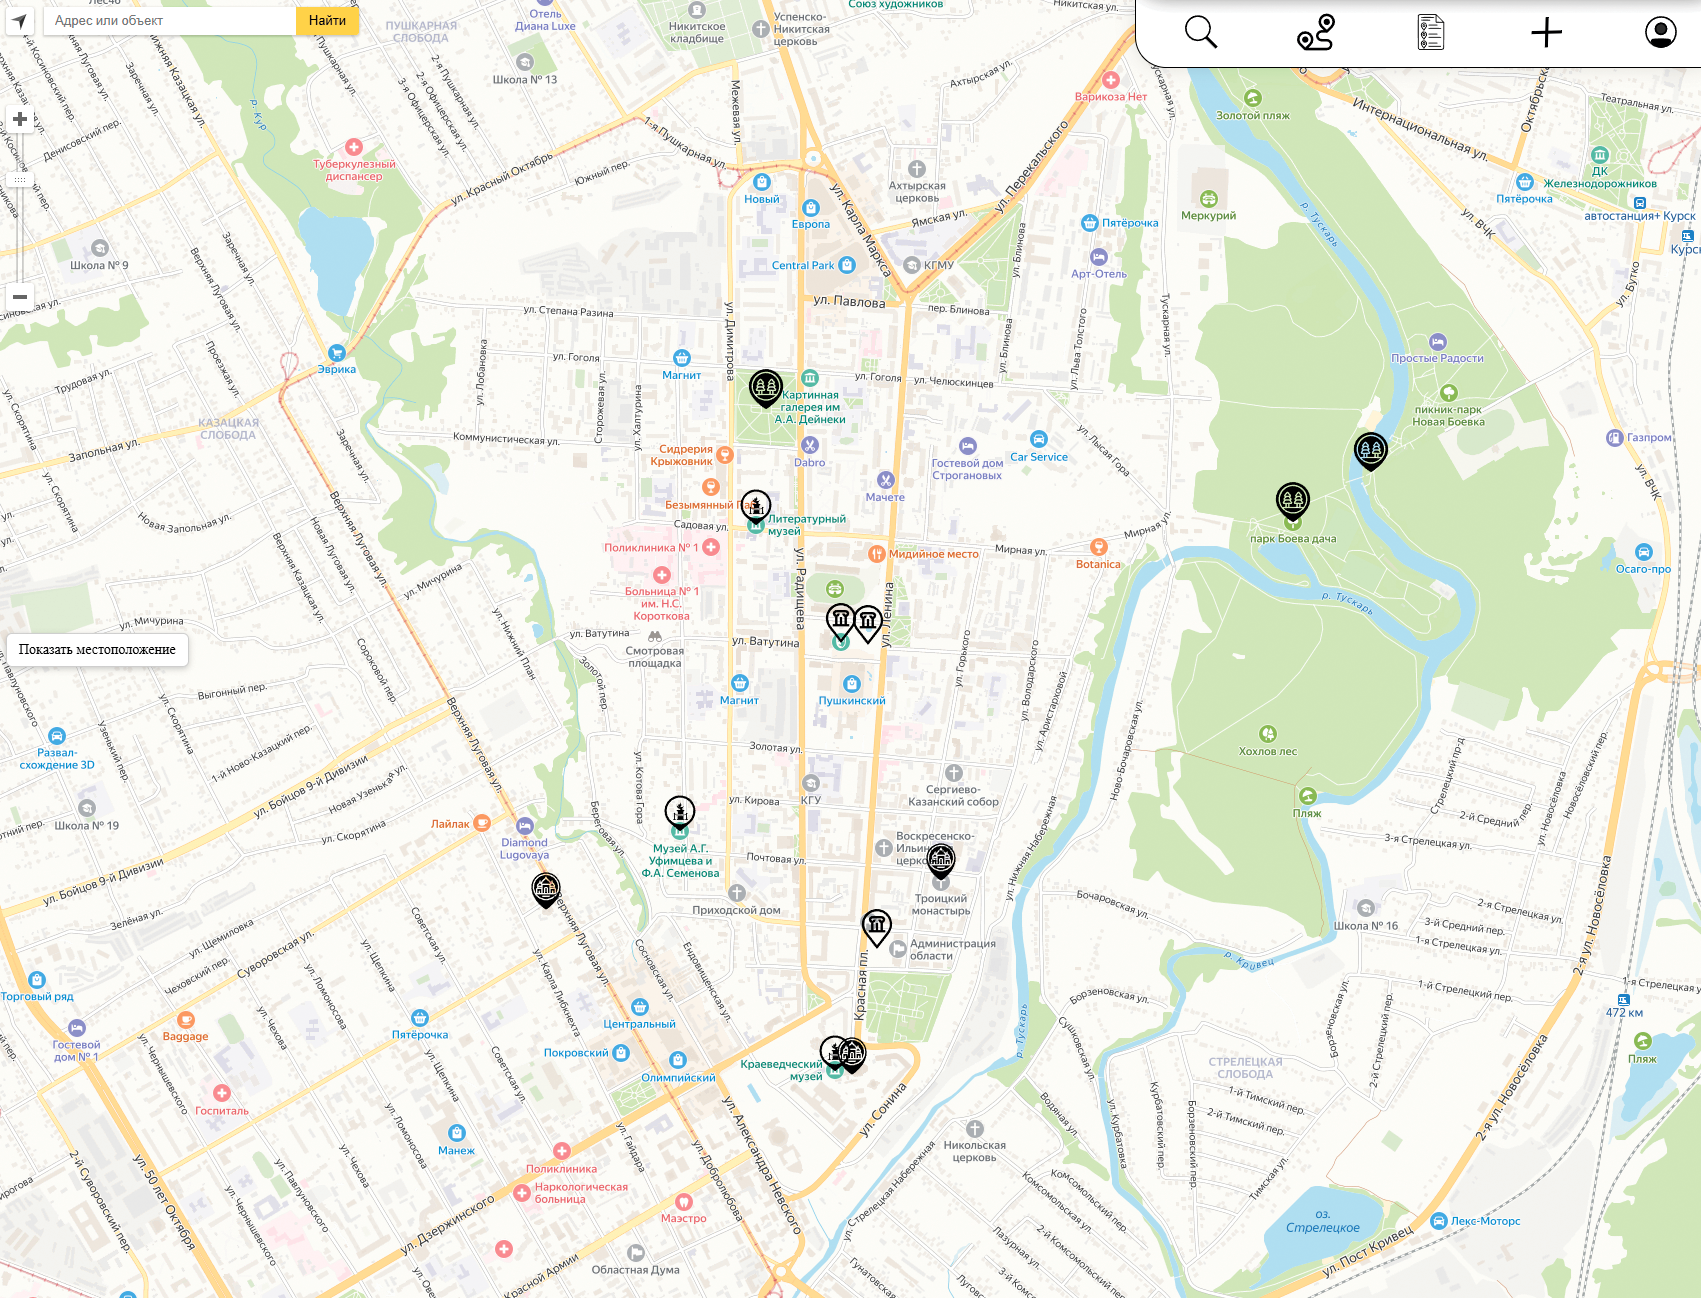
\includegraphics[width=1\linewidth]{r1}}
\caption{Главная страница веб-приложения}
\label{r1:image}
\end{figure}

\newpage
На рисунке \ref{r2:image} представлен поиск туристического объекта по названию.

\begin{figure}[H]
\center{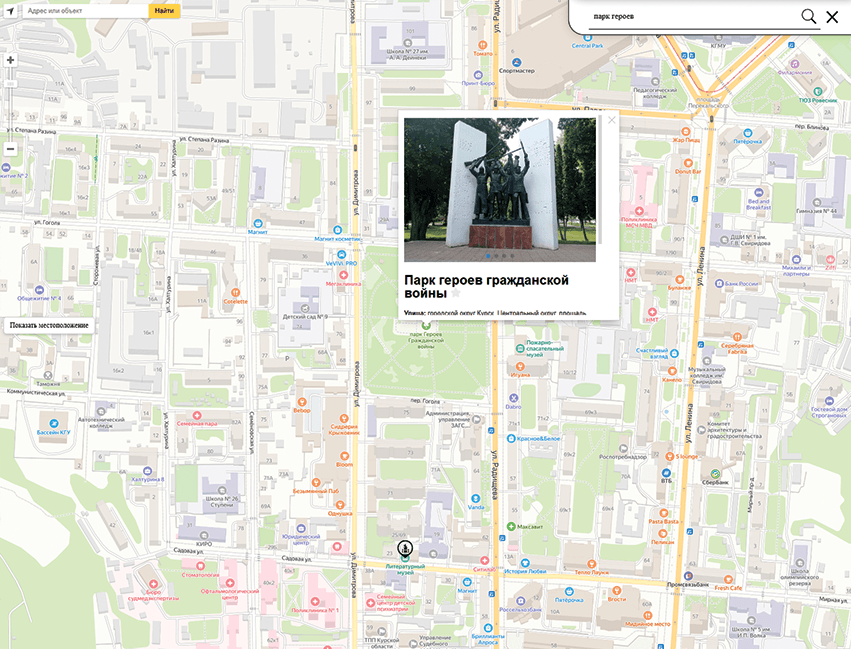
\includegraphics[width=0.8\linewidth]{r2}}
\caption{Поиск туристического объекта по названию}
\label{r2:image}
\end{figure}

На рисунке \ref{r3:image} представлен составленный пользователем маршрут.

\begin{figure}[H]
\center{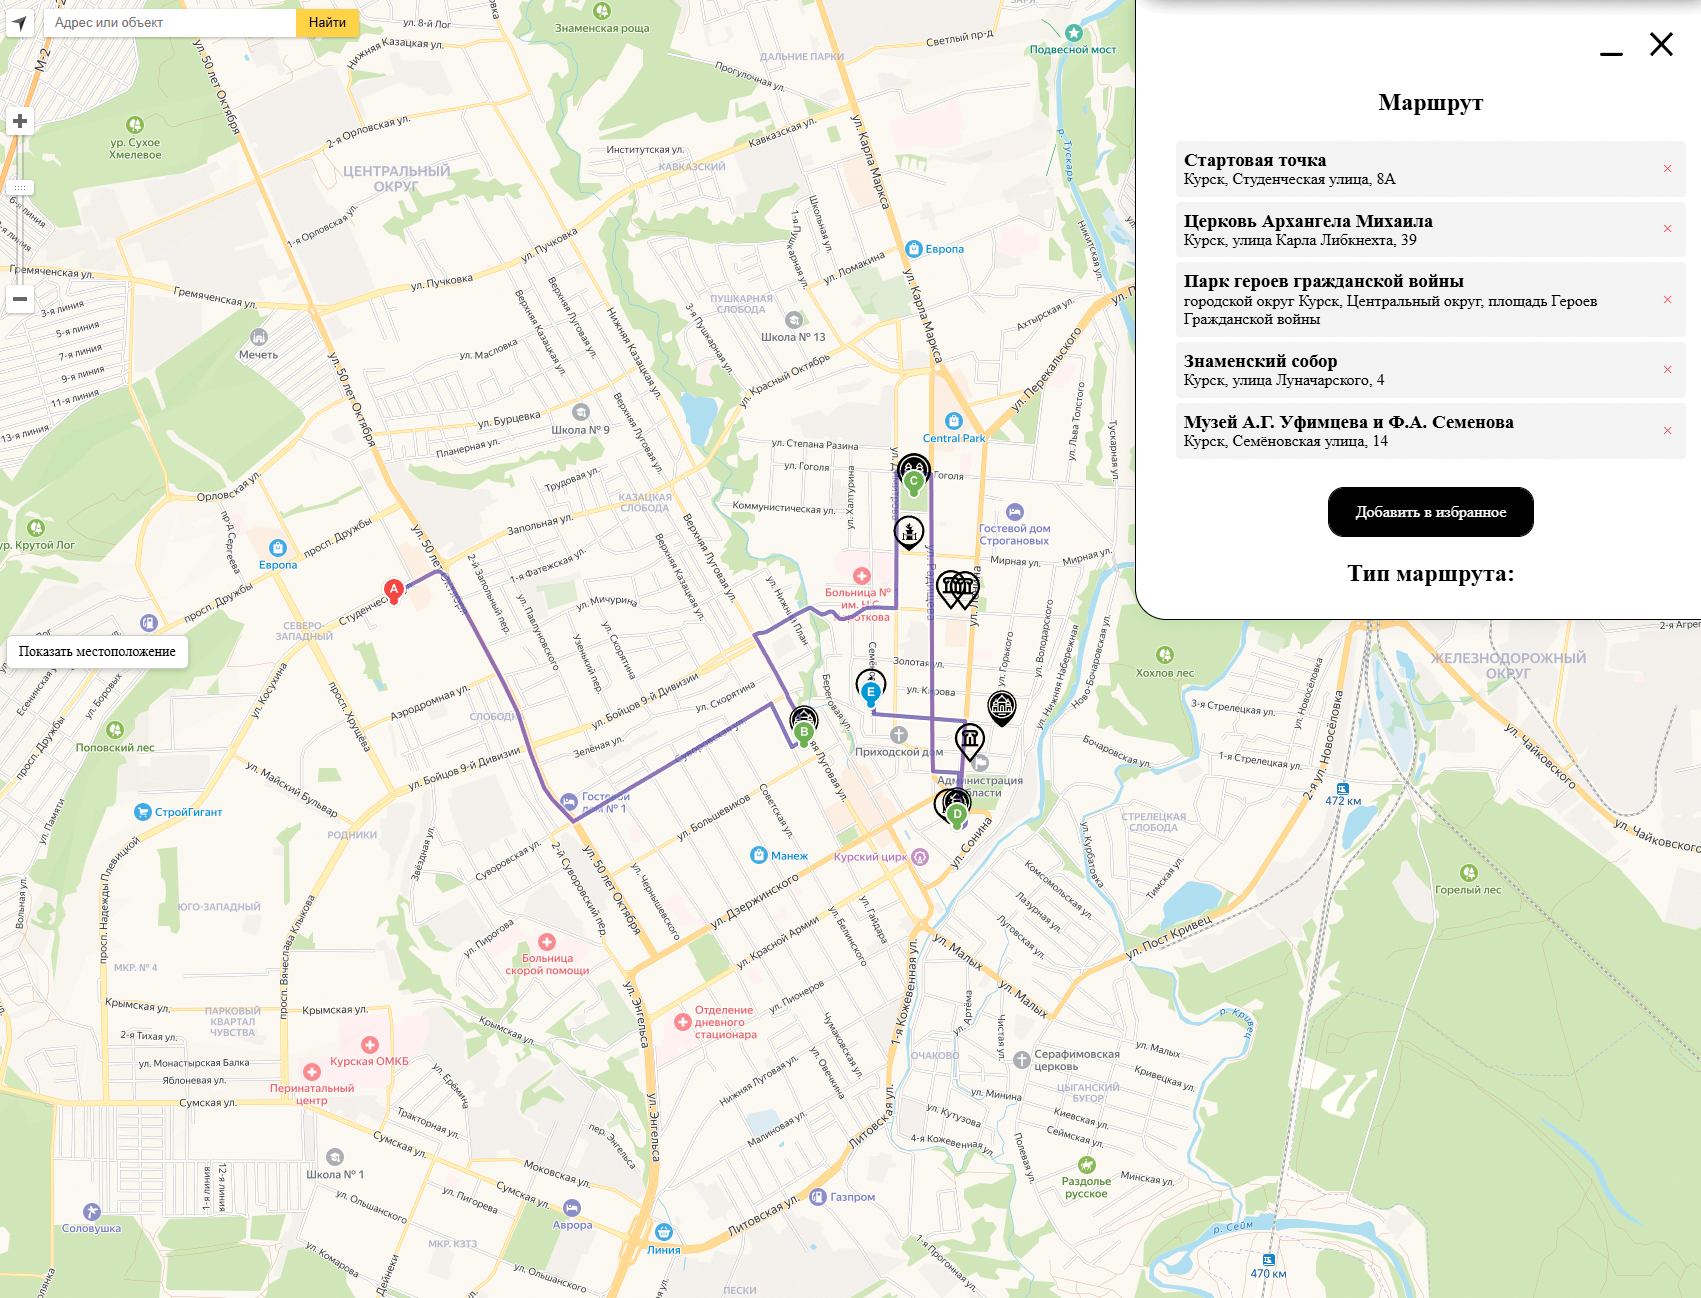
\includegraphics[width=0.8\linewidth]{r3}}
\caption{Пользовательский маршрут}
\label{r3:image}
\end{figure}

\newpage
На рисунке \ref{r4:image} представлено переключение типа маршрута с автомобильного на пешеходный.

\begin{figure}[H]
	\center{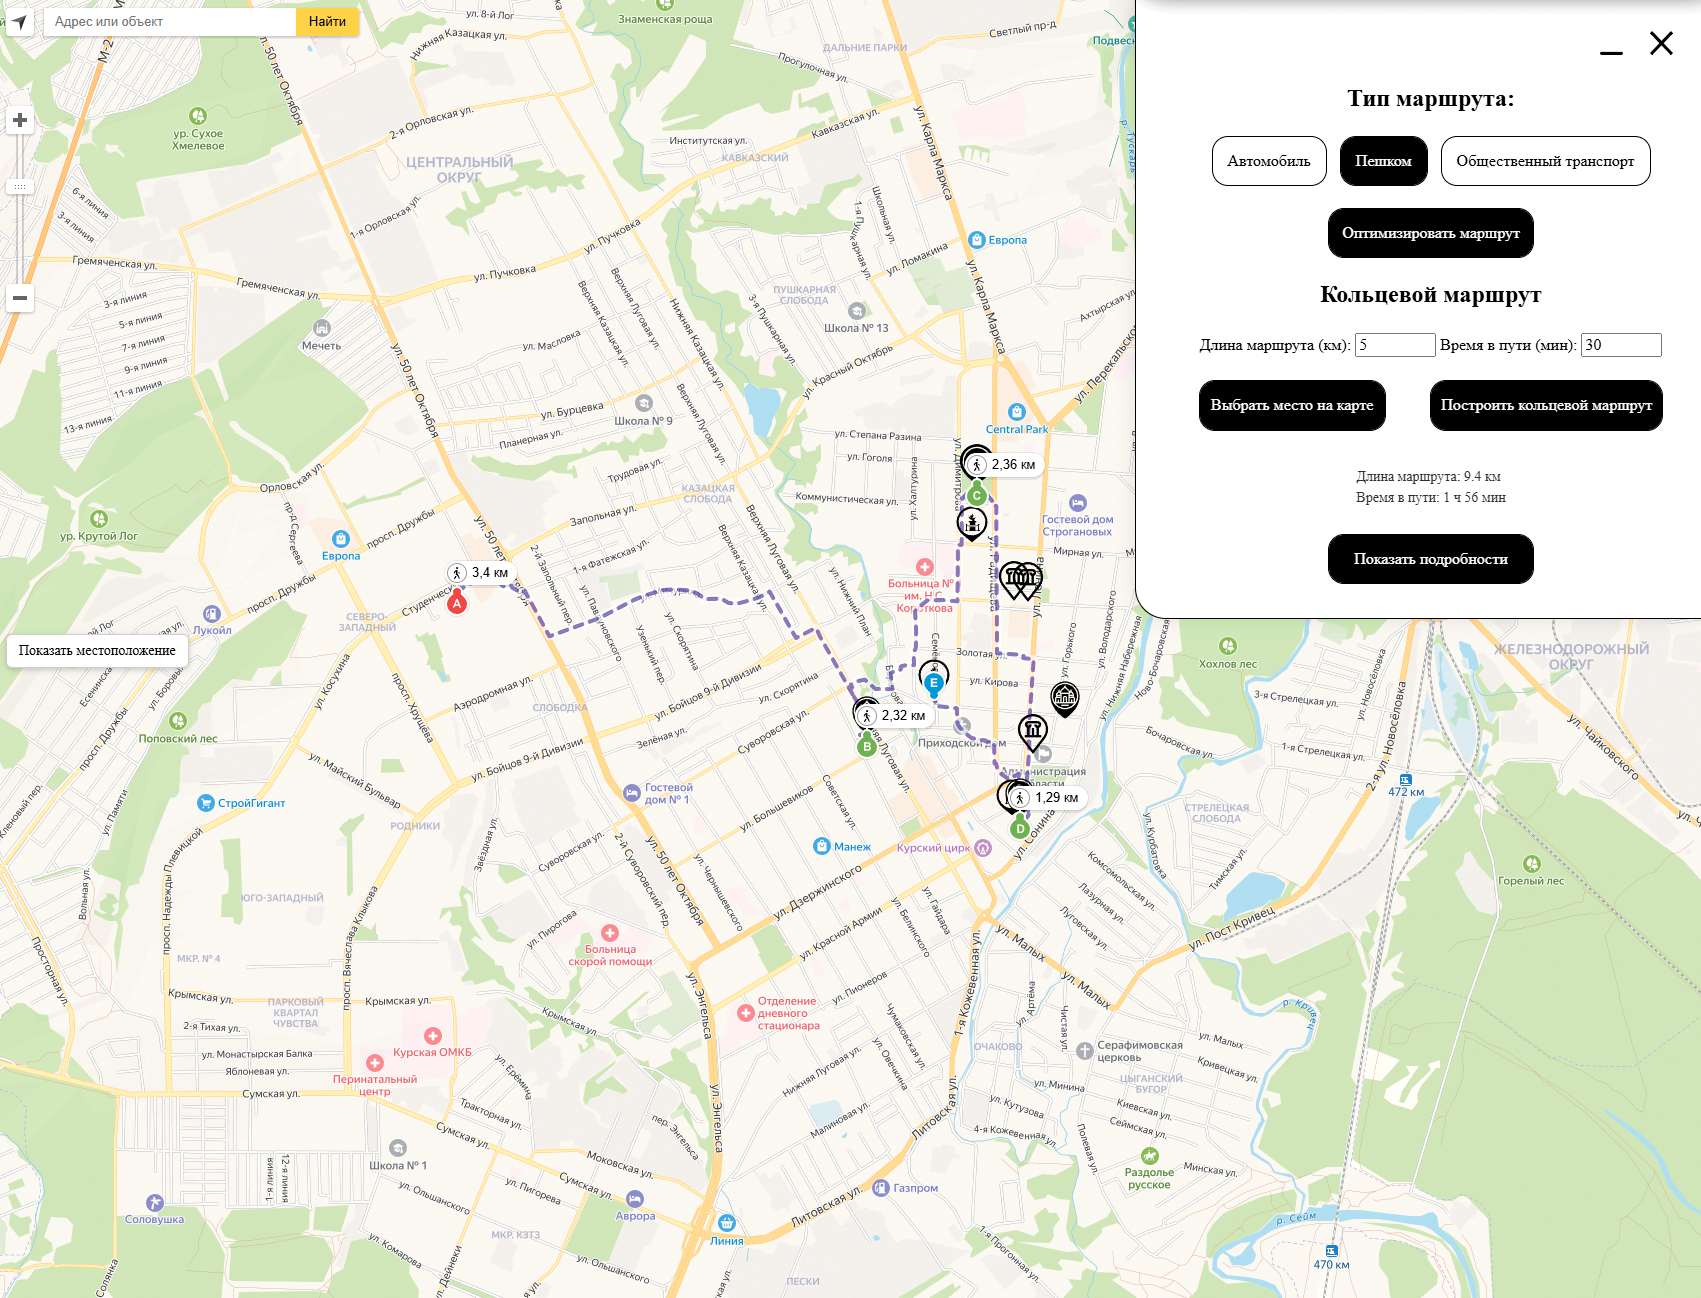
\includegraphics[width=0.8\linewidth]{r4}}
	\caption{Переключение типа маршрута}
	\label{r4:image}
\end{figure}


На рисунке \ref{r11:image} представлена автоматическая оптимизация маршрута.

\begin{figure}[H]
	\center{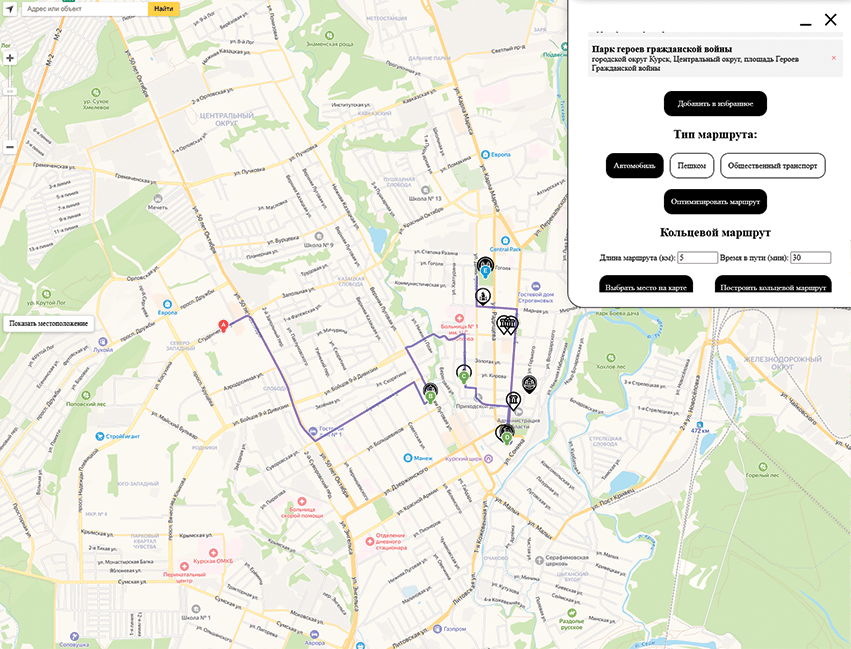
\includegraphics[width=0.8\linewidth]{r11}}
	\caption{Оптимизированный маршрут}
	\label{r11:image}
\end{figure}

\newpage
На рисунке \ref{r5:image} представлена автоматическая генерацию кольцевого маршрута по указанным пользователем параметрам.

\begin{figure}[H]
	\center{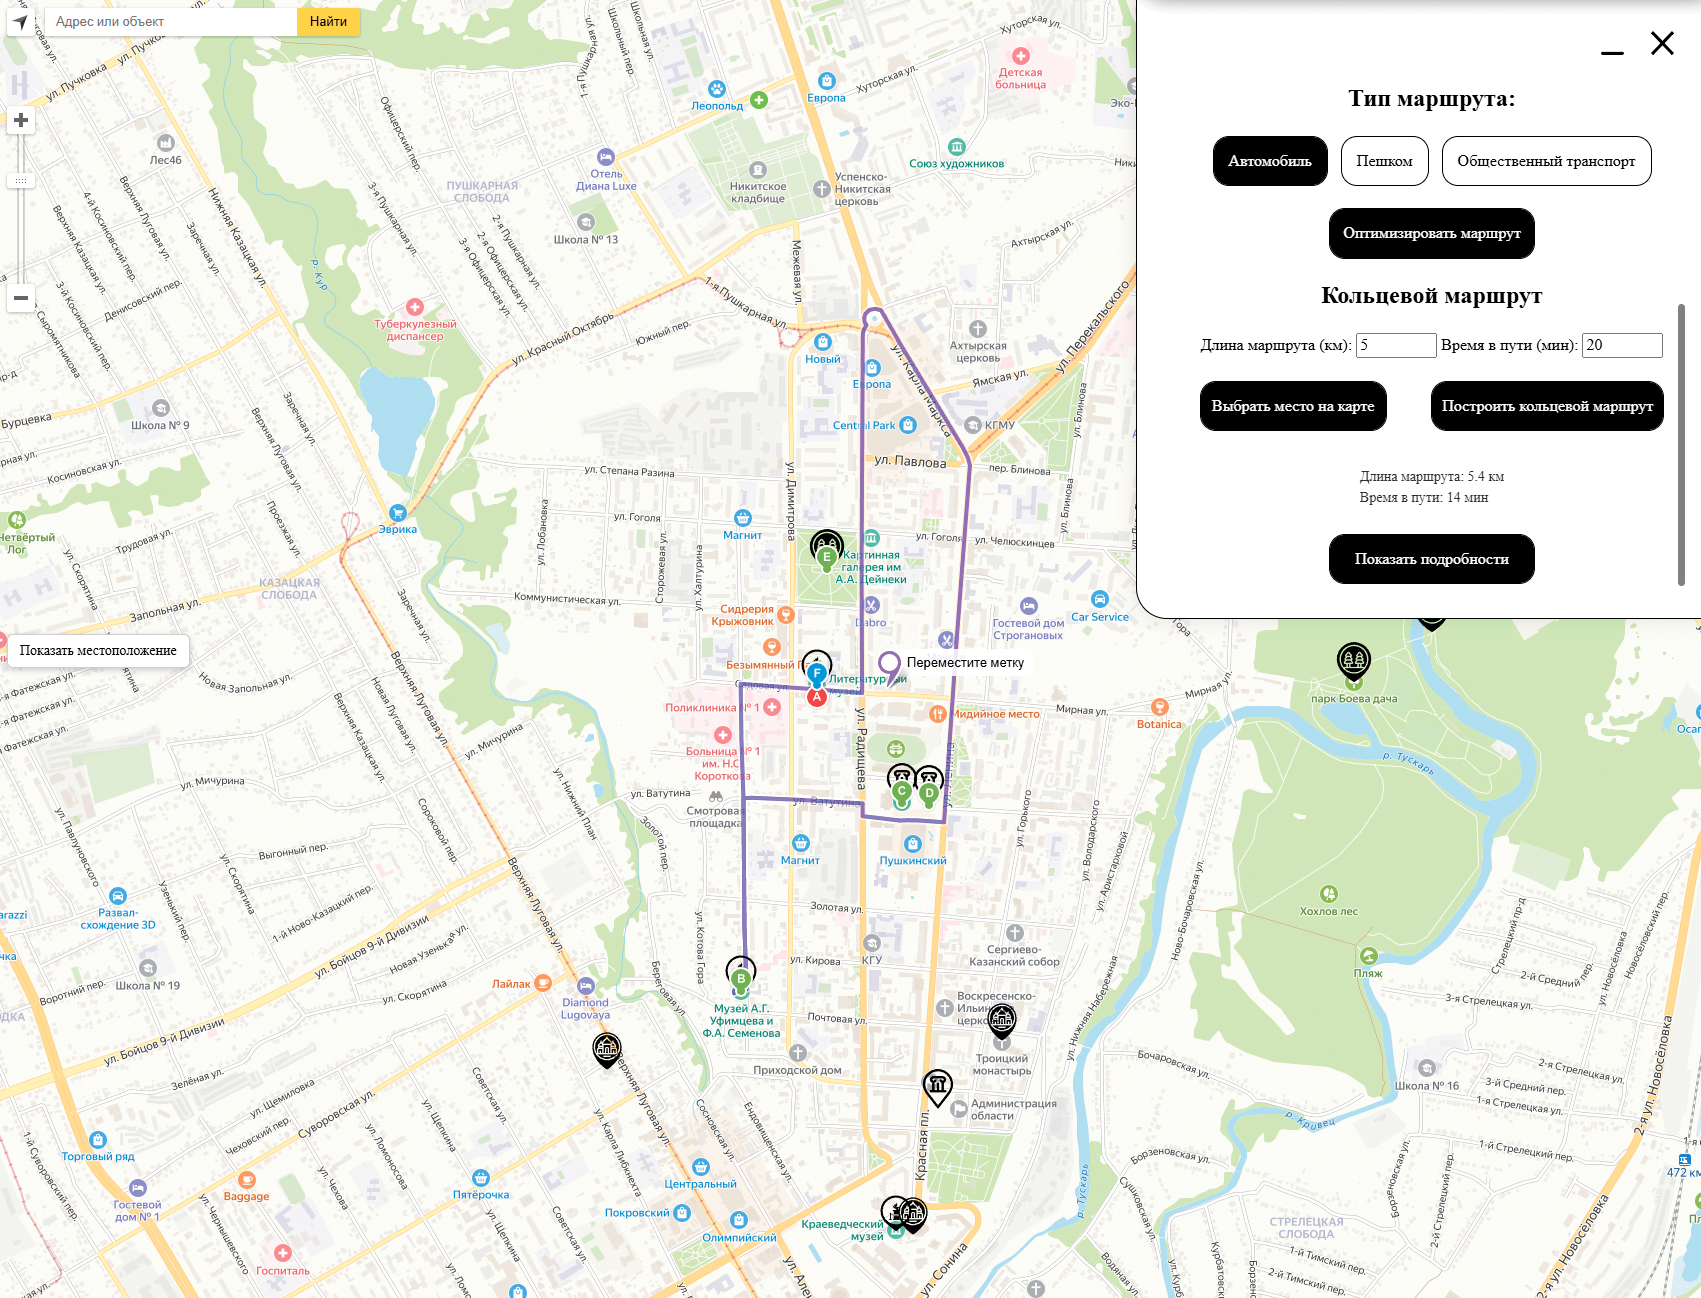
\includegraphics[width=1\linewidth]{r5}}
	\caption{Кольцевой маршрут}
	\label{r5:image}
\end{figure}

\newpage
На рисунке \ref{r6:image} представлена фильтрация объектов на карте.

\begin{figure}[H]
	\center{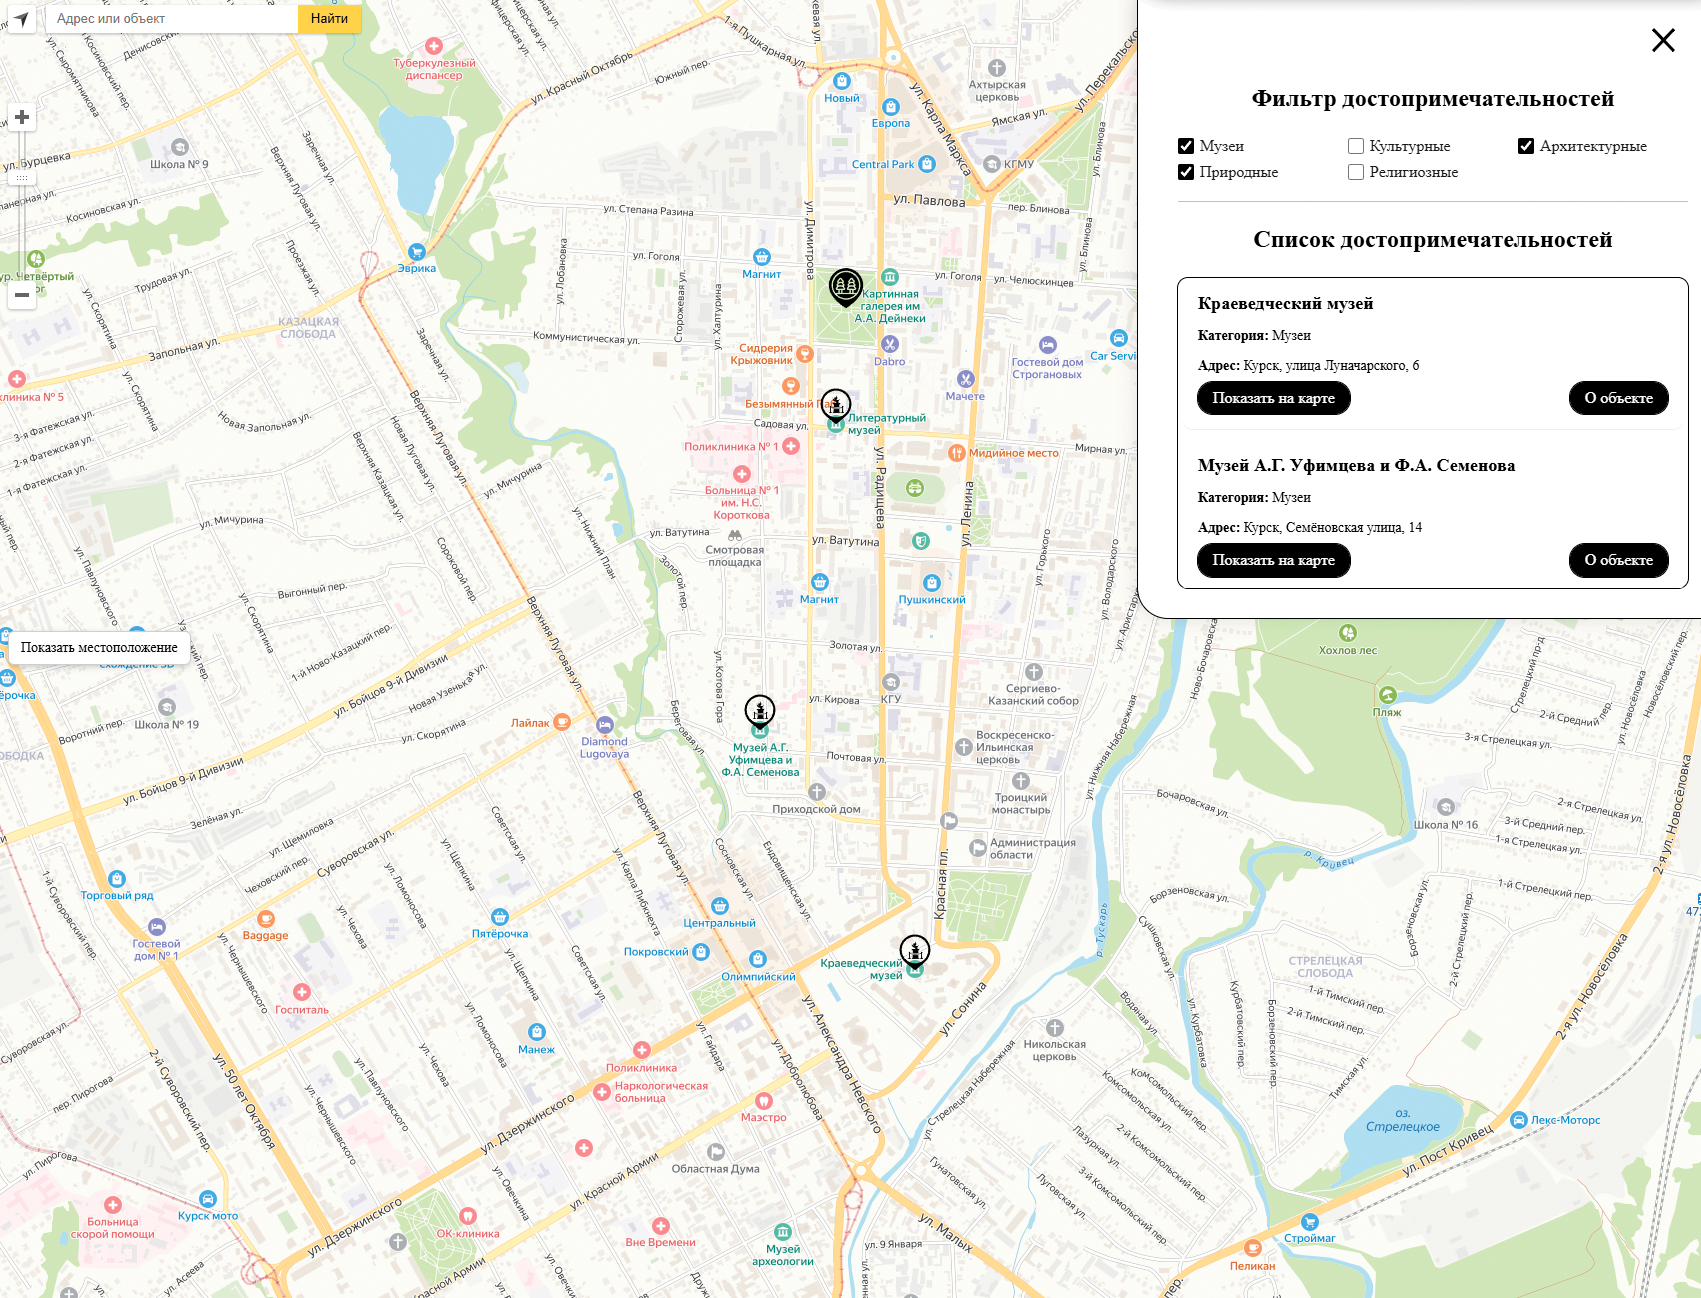
\includegraphics[width=0.8\linewidth]{r6}}
	\caption{Фильтрация объектов}
	\label{r6:image}
\end{figure}

На рисунке \ref{r7:image} представлено определение местоположения пользователя.

\begin{figure}[H]
	\center{
\includegraphics[width=0.5\linewidth]{r7}}
	\caption{Определение местоположения пользователя}
	\label{r7:image}
\end{figure}

\newpage
На рисунке \ref{r8:image} представлена регистрация нового пользователя.

\begin{figure}[H]
	\center{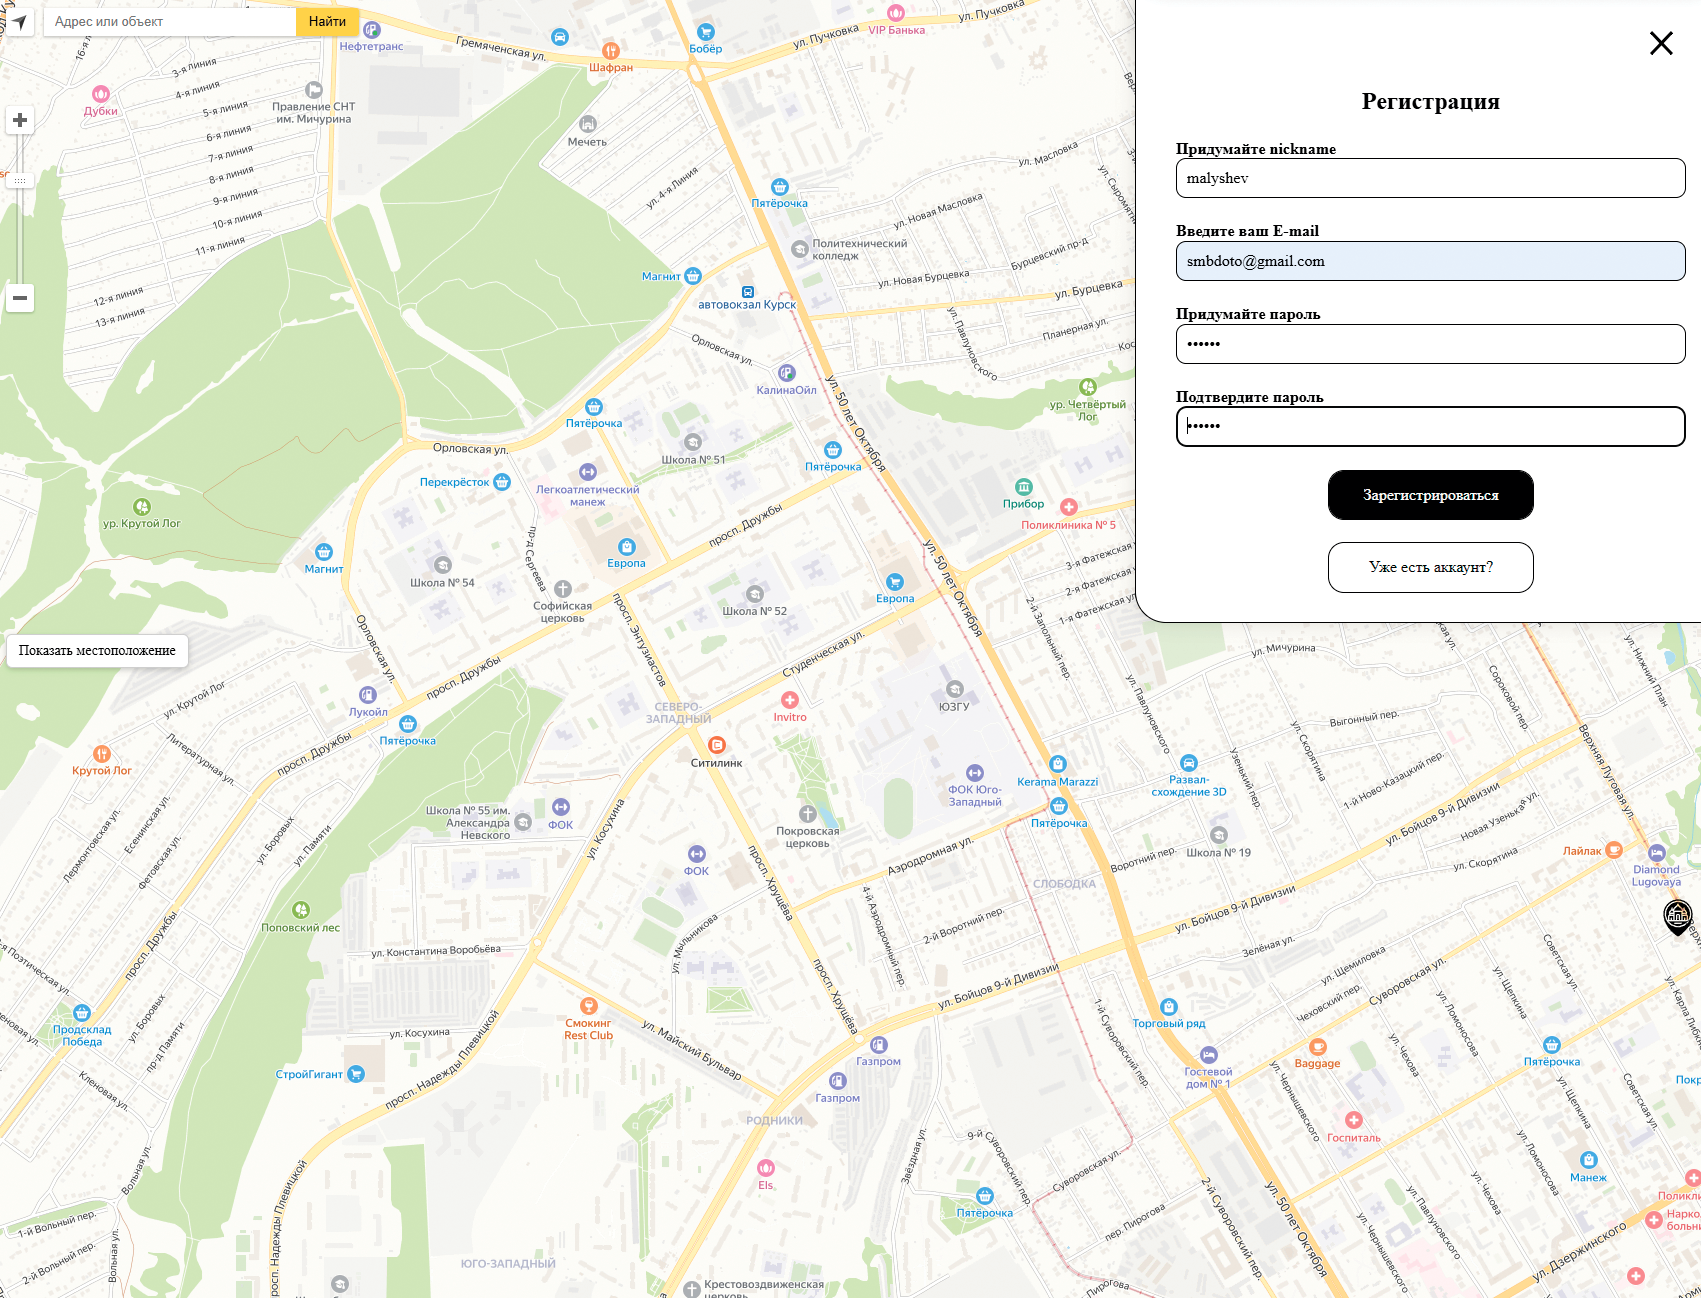
\includegraphics[width=0.6\linewidth]{r8}}
	\caption{Регистрация пользователя}
	\label{r8:image}
\end{figure}

На рисунке \ref{r9:image} представлен вход пользователя в личный кабинет.

\begin{figure}[H]
	\center{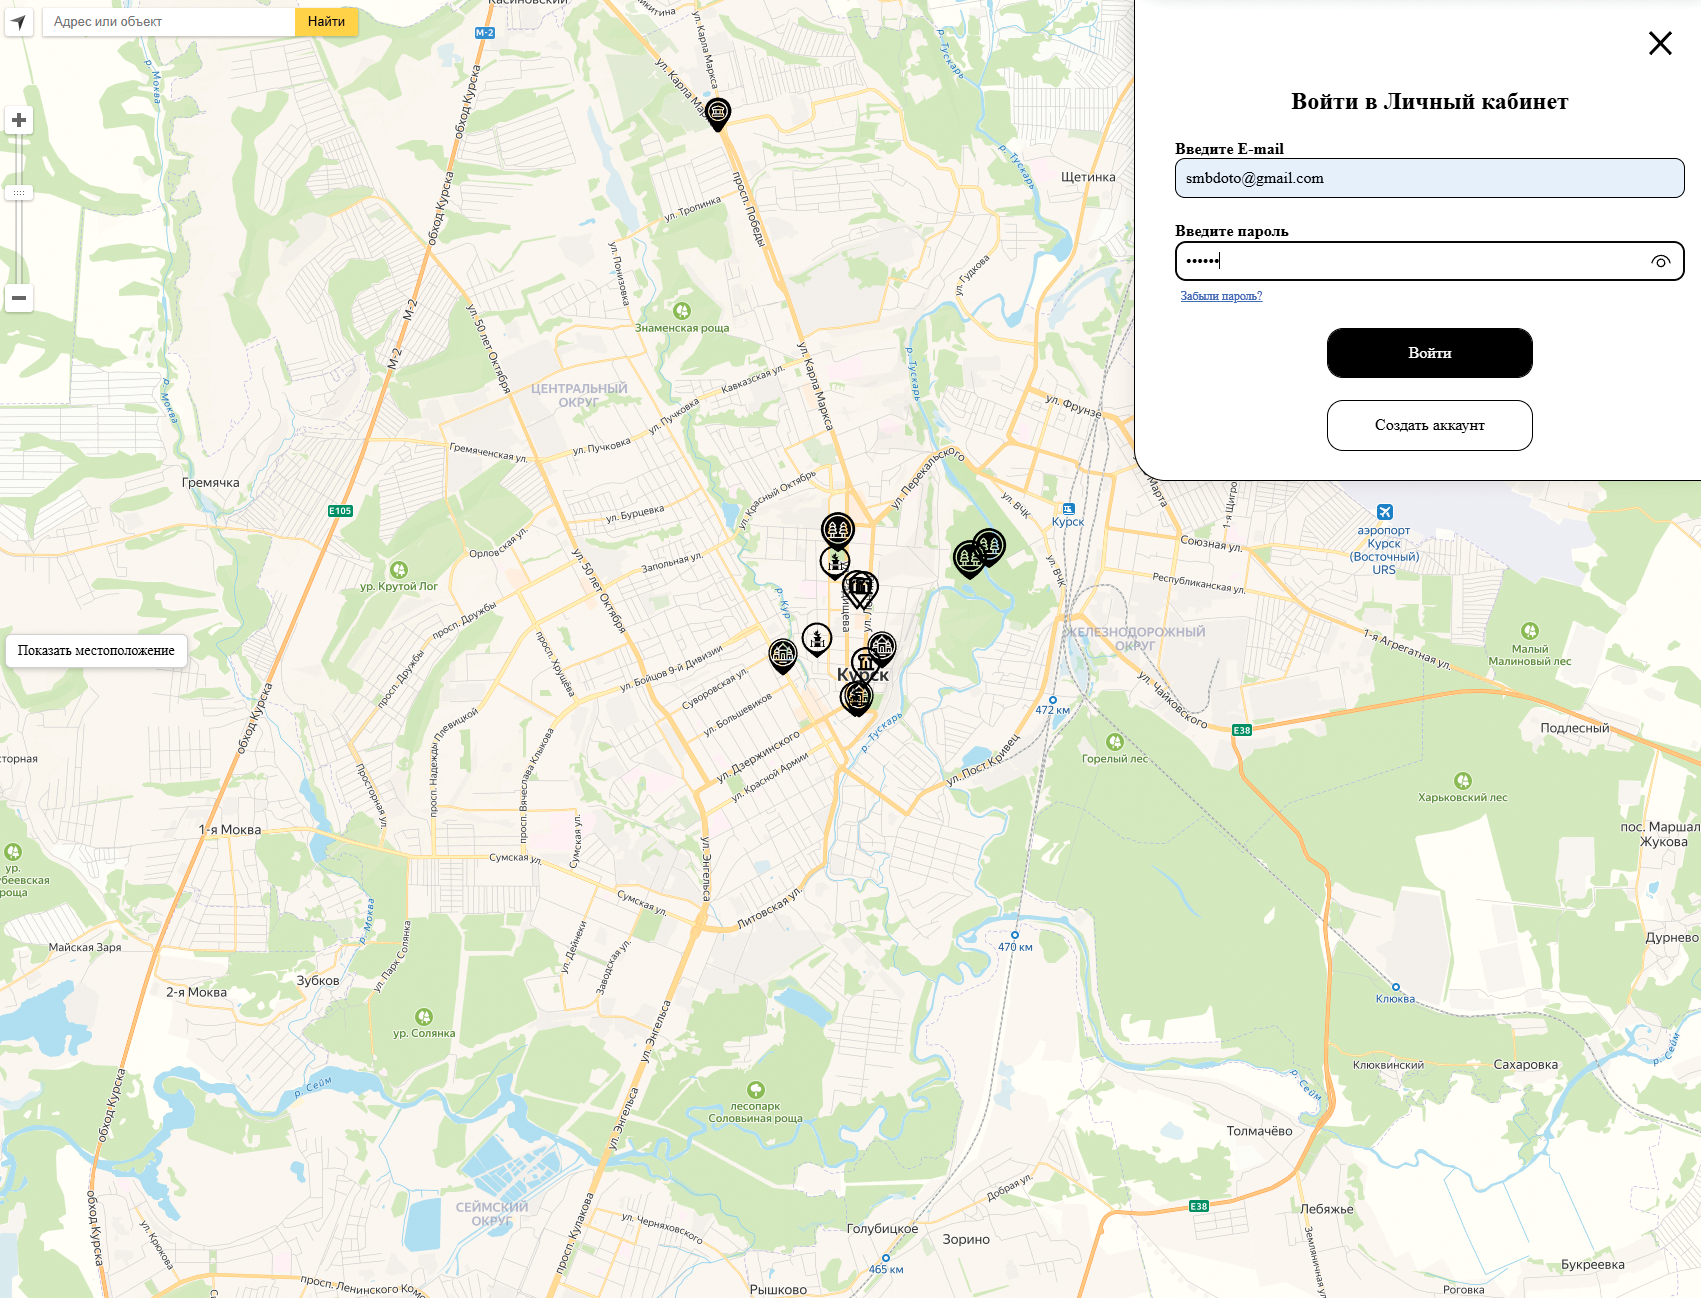
\includegraphics[width=0.6\linewidth]{r9}}
	\caption{Вход в личный кабинет}
	\label{r9:image}
\end{figure}

\newpage
На рисунке \ref{r10:image} представлено сохранение избранных мест пользователя.

\begin{figure}[H]
	\center{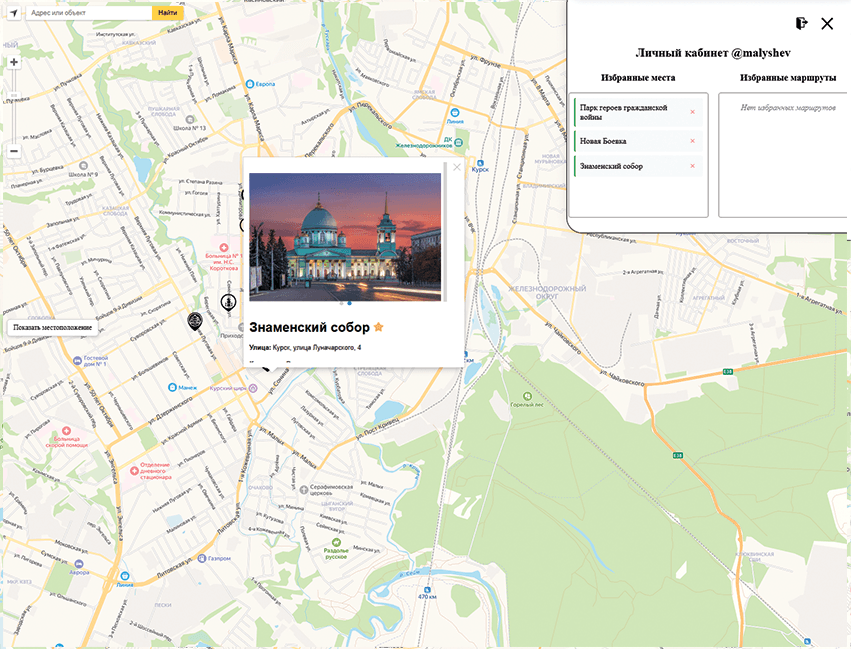
\includegraphics[width=0.85\linewidth]{r10}}
	\caption{Избранные места}
	\label{r10:image}
\end{figure}

На рисунке \ref{r12:image} представлено сохранение избранного маршрута.

\begin{figure}[H]
	\center{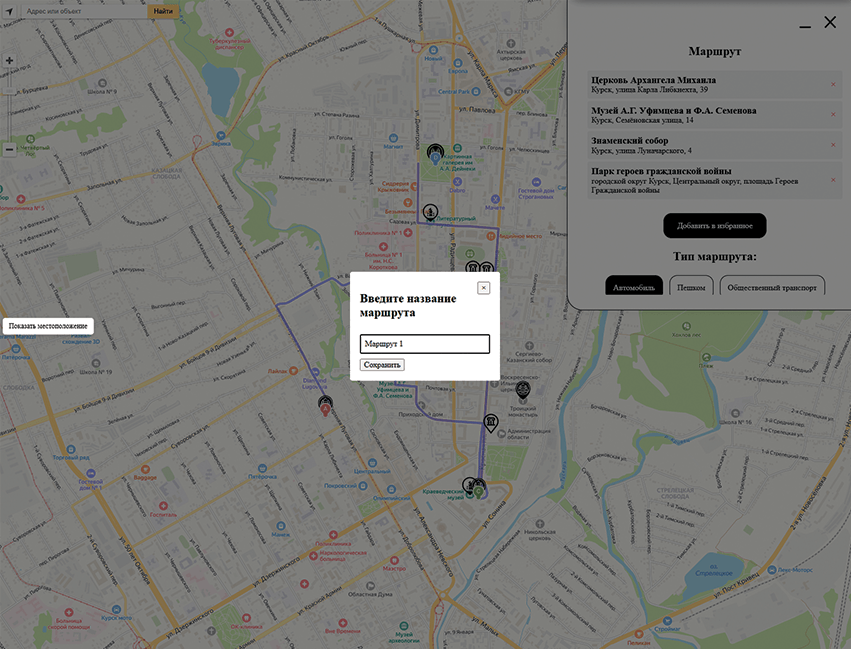
\includegraphics[width=0.45\linewidth]{r12}}
	\caption{Сохранение маршрута}
	\label{r12:image}
\end{figure}

\newpage
На рисунке \ref{r13:image} представлено отображение маршрута в личном кабинете.

\begin{figure}[H]
	\center{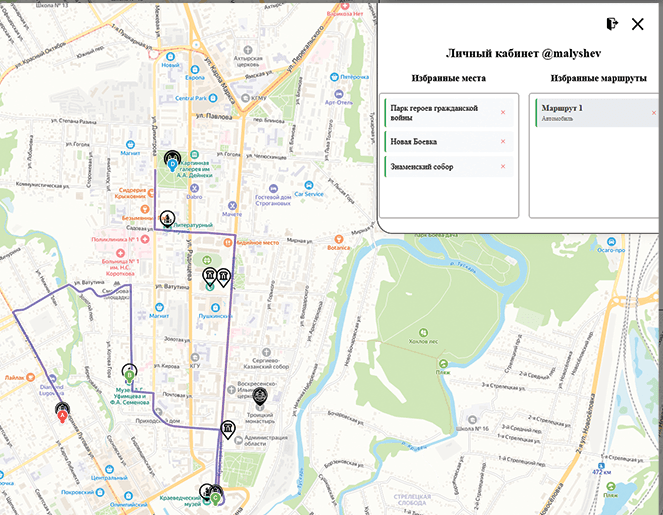
\includegraphics[width=0.8\linewidth]{r13}}
	\caption{Избранные маршруты}
	\label{r13:image}
\end{figure}

На рисунке \ref{r14:image} представлено добавление нового объекта на карту.

\begin{figure}[H]
	\center{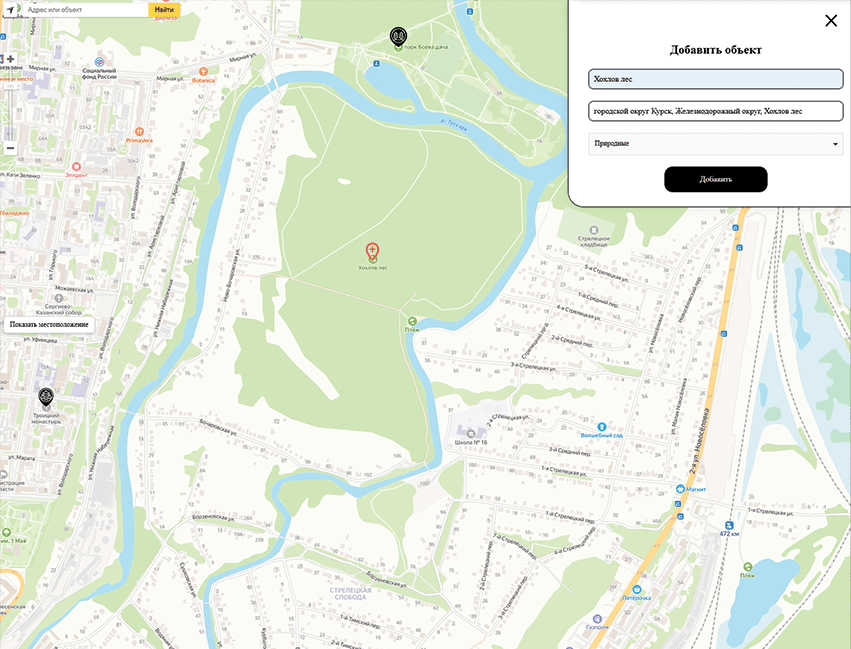
\includegraphics[width=0.8\linewidth]{r14}}
	\caption{Добавление нового объекта}
	\label{r14:image}
\end{figure}

\newpage
На рисунке \ref{r15:image} представлена проверка нового места администратором.

\begin{figure}[H]
	\center{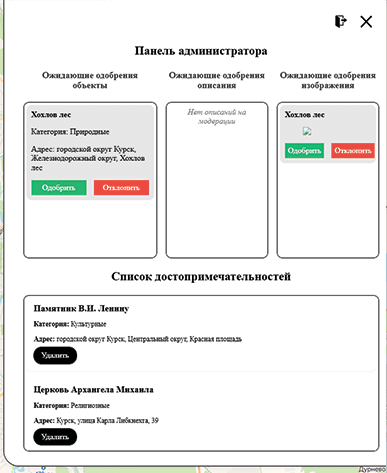
\includegraphics[width=0.5\linewidth]{r15}}
	\caption{Панель администратора}
	\label{r15:image}
\end{figure}

На рисунке \ref{r16:image} представлено появление нового объекта на карте, после одобрения.

\begin{figure}[H]
	\center{
\includegraphics[width=0.4\linewidth]{r16}}
	\caption{Появление нового объекта на карте}
	\label{r16:image}
\end{figure}

\newpage
На рисунке \ref{r17:image} представлено добавление описания для объекта, если это делает администратор, проверки не требуется.

\begin{figure}[H]
	\center{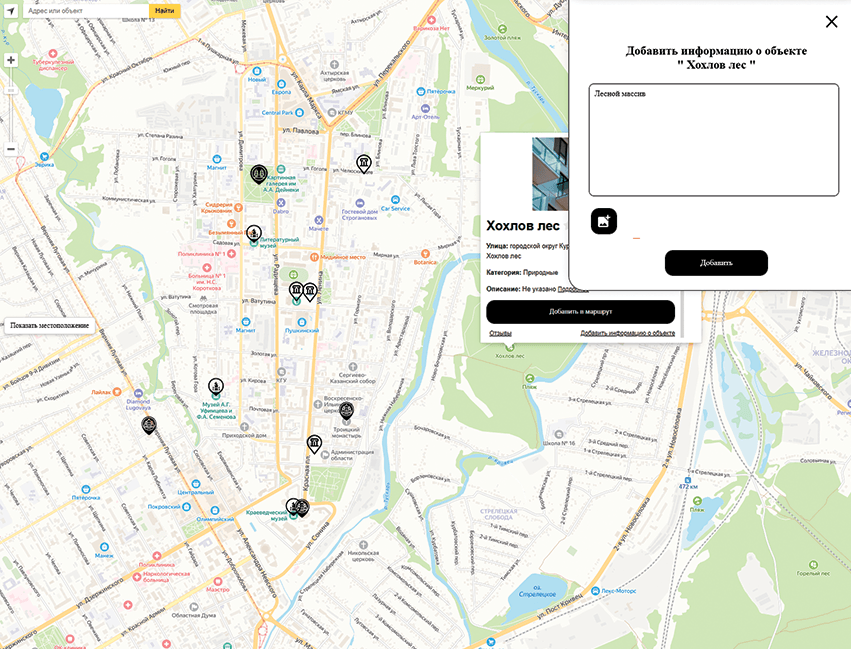
\includegraphics[width=0.7\linewidth]{r17}}
	\caption{Добавление описания}
	\label{r17:image}
\end{figure}

На рисунке \ref{r18:image} представлено новое описание объекта.

\begin{figure}[H]
	\center{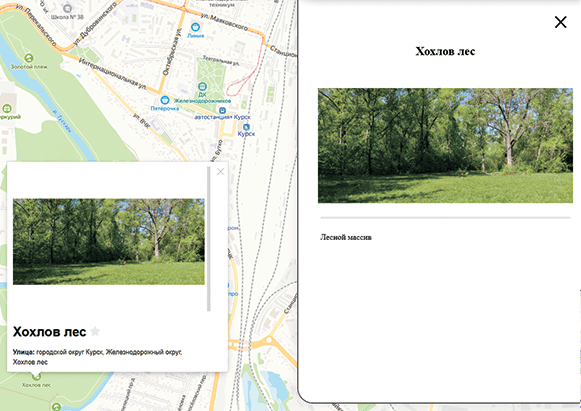
\includegraphics[width=0.7\linewidth]{r18}}
	\caption{Новое описание объекта}
	\label{r18:image}
\end{figure}

\newpage
На рисунке \ref{r19:image} представлена панель отзывов об объекте.

\begin{figure}[H]
	\center{
\includegraphics[width=1\linewidth]{r19}}
	\caption{Панель отзывов}
	\label{r19:image}
\end{figure}

На рисунке \ref{r20:image} представлено добавление нового отзыва об объекте.

\begin{figure}[H]
	\center{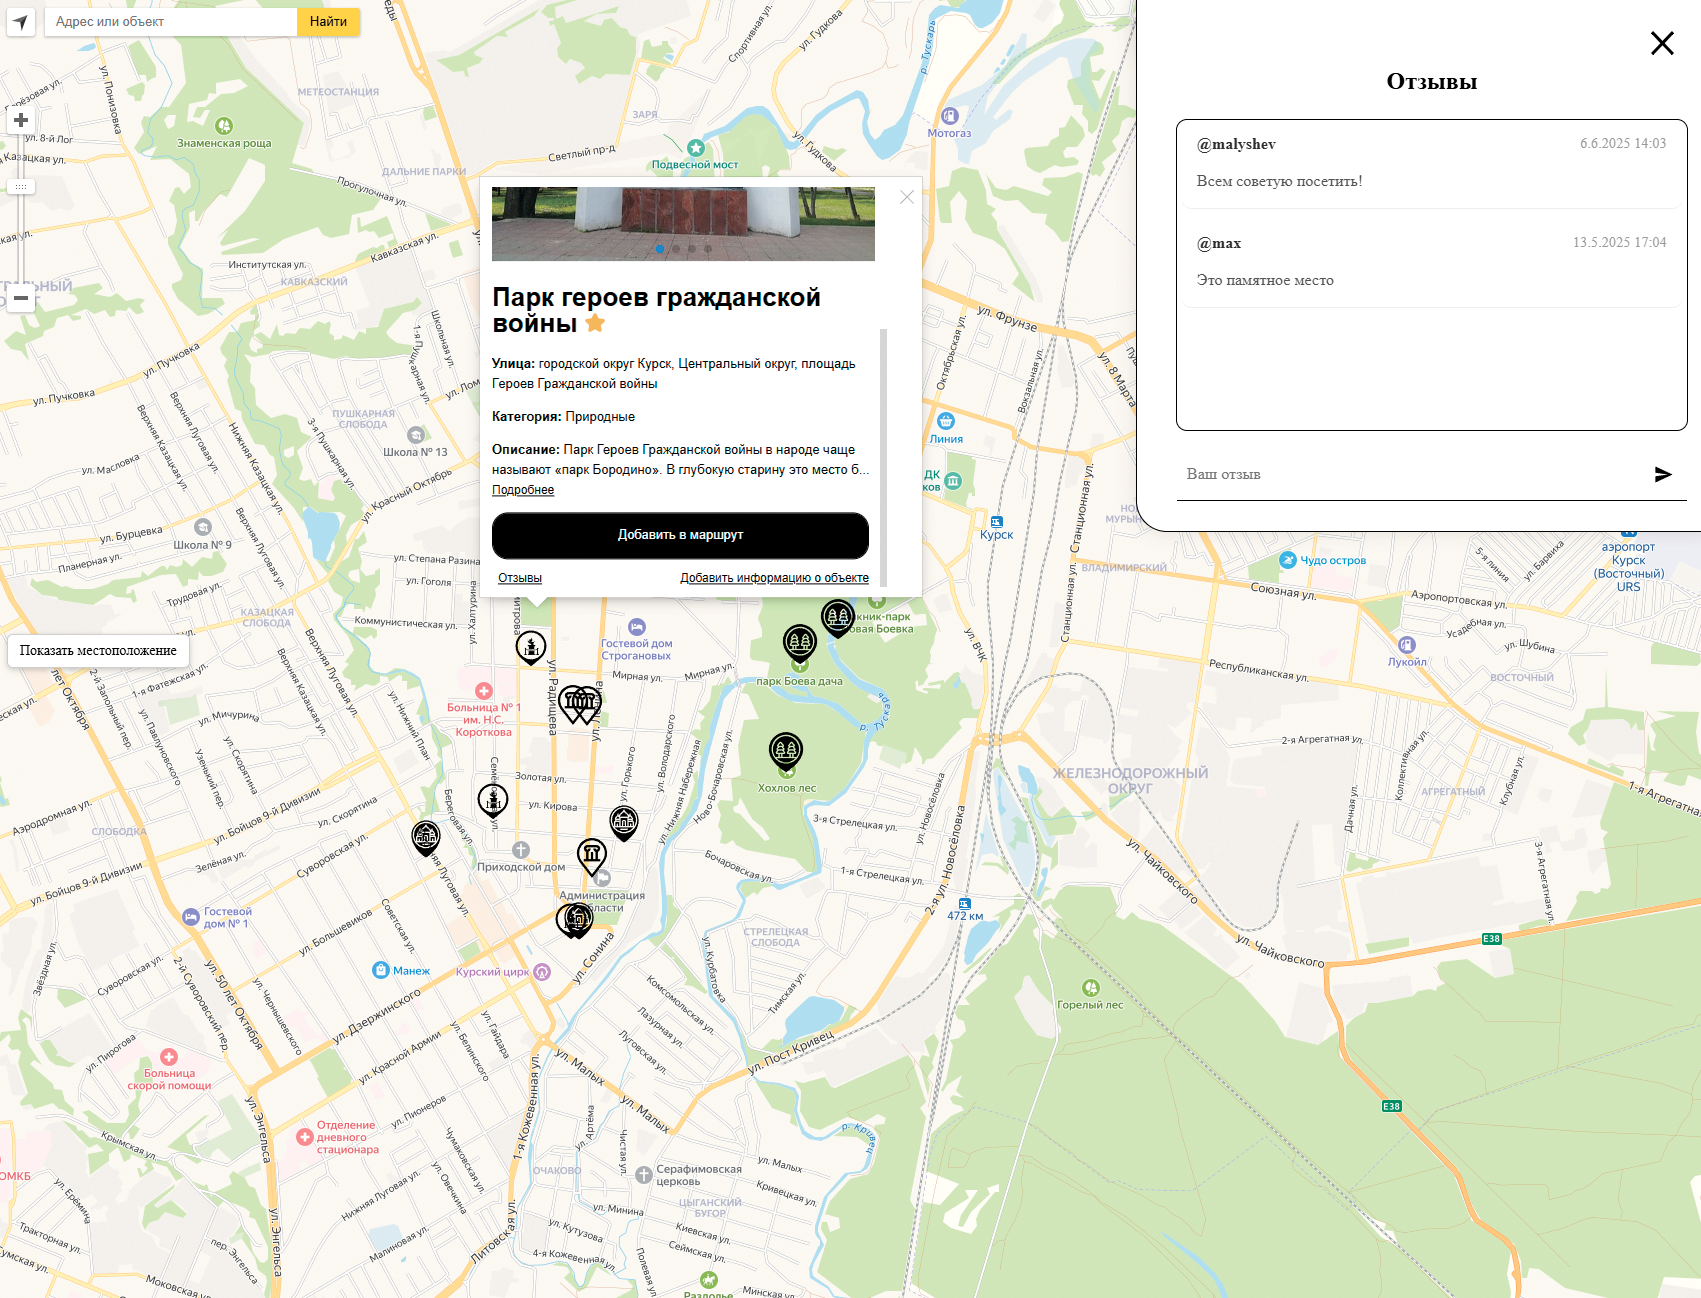
\includegraphics[width=1\linewidth]{r20}}
	\caption{Добавление нового отзыва}
	\label{r20:image}
\end{figure}

\subsection{Сборка компонентов программной системы}

На заключительном этапе разработки осуществляется объединение всех разработанных компонентов в единую, целостную программную систему. Сборка включает настройку взаимосвязей между модулями, интеграцию клиентской и серверной части, подключение внешних API, а также развёртывание проекта в рабочей среде. Этот процесс требует особой внимательности, так как от согласованной работы всех частей напрямую зависит стабильность и надёжность всего приложения\cite{b29}.

В рамках настоящего проекта сборка компонентов осуществлялась поэтапно. Сначала были интегрированы скрипты визуализации и взаимодействия с картой, реализованные на JavaScript с использованием API Яндекс.Карт. Далее подключены модули обработки пользовательских данных, включая систему авторизации, добавления объектов, отзывов и избранного. Серверная логика на PHP была связана с клиентскими запросами через интерфейс асинхронного обмена данными, обеспечивая быструю реакцию интерфейса без перезагрузки страницы.

Файловая структура проекта была организована по принципу логического разделения ответственности: отдельные каталоги для стилей, сценариев, изображений и обработчиков данных. Это обеспечило не только удобство сопровождения, но и упростило процесс масштабирования проекта в будущем. Все компоненты, включая формы, фильтры, модальные окна, навигационные панели и маршрутизаторы, были приведены к единому стилю и протестированы на совместимость.

После завершения сборки система была развернута в тестовой среде, где прошла полную проверку функциональности. Успешное объединение клиентской и серверной логики позволило обеспечить полноценную работу всех функций, предусмотренных техническим заданием, включая отображение объектов на карте, взаимодействие с балунами, построение и сохранение маршрутов\cite{b30}, а также взаимодействие с пользовательскими данными.

Таким образом, сборка компонентов завершила цикл разработки программной системы и обеспечила её готовность к развертыванию в продуктивной среде.

	\section*{ЗАКЛЮЧЕНИЕ}
\addcontentsline{toc}{section}{ЗАКЛЮЧЕНИЕ}

Преимущества аддитивных технологий заключается в разнообразии процессов, позволяющих применять их в различных областях производства. Существенным ограничением же является и экономическая составляющая, которая не позволит внедрить аддитивное производство повсеместно.
  
Компании, видя, как развиваются информационные технологии, пытаются использовать их выгодно для своего бизнеса, запуская свой сайт для того, чтобы заявить о своем существовании, проинформировать потенциального клиента об услугах или продуктах, которые предоставляет. 
Для продвижения компании «Русатом – Аддитивные технологии» был разработан веб-сайт на основе системы «1С-Битрикс: Управление сайтом».

Основные результаты работы:

\begin{enumerate}
\item Проведен анализ предметной области. Выявлена необходимость использовать 1С-Битрикс.
\item Разработана концептуальная модель web-сайта. Разработана модель данных системы. Определены требования к системе.
\item Осуществлено проектирование web-сайта. Разработана архитектура серверной части. Разработан пользовательский интерфейс web-сайта.
\item Реализован и протестирован web-сайт. Проведено модульное и системное тестирование.
\end{enumerate}

Все требования, объявленные в техническом задании, были полностью реализованы, все задачи, поставленные в начале разработки проекта, были также решены.

Готовый рабочий проект представлен адаптивной версткой сайта. Сайт находится в публичном доступе, поскольку опубликован в сети Интернет.  

}\fi
\addcontentsline{toc}{section}{СПИСОК ИСПОЛЬЗОВАННЫХ ИСТОЧНИКОВ}

\begin{thebibliography}{21}

    \bibitem{b1} Фаулер, М. Архитектура корпоративных программных приложений / М. Фаулер. – 3-е изд., перераб. – СПб. : Питер, 2020. – 544 с. – ISBN 978-5-4461-1692-1. – Текст : непосредственный.
   	\bibitem{b2}	Ларсен, У. Архитектура веб-приложений: от монолита к микросервисам / У. Ларсен. – М. : БХВ-Петербург, 2019. – 416 с. – ISBN 978-5-9775-4009-6. – Текст : непосредственный.
   	\bibitem{b3}	Смит, А. Современная JavaScript-разработка: от ES6 до ES2022 / А. Смит. – СПб. : Питер, 2023. – 384 с. – ISBN 978-5-4461-1971-7. – Текст : непосредственный.
    \bibitem{b4}	Сандерс, Р. Node.js. Создание серверных приложений на JavaScript / Р. Сандерс. – СПб. : Питер, 2021. – 320 с. – ISBN 978-5-4461-1605-1. – Текст : непосредственный.
   	\bibitem{b5}	Mozilla Developer Network : Web APIs : сайт. – URL: https://developer.mozilla.org/en-US/docs/Web/API (дата обращения: 01.05.2025). – Текст : электронный.
	\bibitem{b6}	Джонсон, Д. Веб-дизайн: современные подходы к созданию интерфейсов / Д. Джонсон. – М. : Эксмо, 2020. – 352 с. – ISBN 978-5-04-108539-9. – Текст : непосредственный.
	\bibitem{b7} Норман, Д. Дизайн привычных вещей / Д. Норман. – М. : Манн, Иванов и Фербер, 2016. – 384 с. – ISBN 978-5-00057-684-7. – Текст : непосредственный.
   	\bibitem{b8}	Рейнджер, М. Проектирование пользовательского опыта: Руководство по UX / М. Рейнджер. – М. : Альпина Паблишер, 2021. – 278 с. – ISBN 978-5-9614-7183-3. – Текст : непосредственный.    
	\bibitem{b9} Бозетти, Ф. UX Design 2022: Руководство по проектированию пользовательского интерфейса / Ф. Бозетти. – Independently Published, 2022. – 206 с. – ISBN 979-8-3912-8453-0. – Текст : непосредственный.
	\bibitem{b10}	Коупленд, Л. Архитектура REST API. Проектирование надёжных веб-сервисов / Л. Коупленд. – М. : Диалектика, 2018. – 288 с. – ISBN 978-5-8459-2006-4. – Текст : непосредственный.
 	\bibitem{b11} Яндекс.Карты API : JavaScript API 2.1 : сайт. – URL: https://yandex.ru/dev/maps/jsapi/doc/2.1/quick-start/ (дата обращения: 27.04.2025). – Текст : электронный.
 	\bibitem{b12}	Вуд, А. CSS: Секреты профессионалов. 2-е изд. / А. Вуд. – М. : Питер, 2019. – 400 с. – ISBN 978-5-4461-1383-8. – Текст : непосредственный.
 	\bibitem{b13} Сноу, М. Архитектура клиент-серверных приложений: современные подходы и технологии / М. Сноу. – СПб. : Диалектика, 2021. – 312 с. – ISBN 978-5-6046702-3-4. – Текст : непосредственный.	
 	\bibitem{b19} HTML Living Standard : WHATWG specification : сайт. – URL: https://html.spec.whatwg.org/ (дата обращения: 21.04.2025). – Текст : электронный.
 	\bibitem{b18} Фланаган, Д. JavaScript. Подробное руководство. 7-е изд. / Д. Фланаган. – М. : Вильямс, 2021. – 960 с. – ISBN 978-5-8459-2231-0. – Текст : непосредственный.
	\bibitem{b14}	Хартманн, К. Базы данных для веб-разработчиков: от SQL до NoSQL / К. Хартманн. – СПб. : БХВ-Петербург, 2020. – 352 с. – ISBN 978-5-9775-4055-3. – Текст : непосредственный. 
	\bibitem{b15} Nielsen, J. Usability Engineering / J. Nielsen. – Morgan Kaufmann, 2016. – 362 p. – ISBN 978-0125184069. – Текст : непосредственный.
	\bibitem{b16} MDN Web Docs: Cascading Style Sheets (CSS) : сайт. – URL: https://developer.mozilla.org/en-US/docs/Web/CSS (дата обращения: 02.05.2025). – Текст : электронный.
	\bibitem{b17} JavaScript: The Definitive Guide / Д. Флэнаган. – 7-е изд. – O’Reilly Media, 2020. – 706 с. – ISBN 978-1-4919-5542-8. – Текст : непосредственный.
	
	\bibitem{b20} Cooper, A. About Face: The Essentials of Interaction Design / A. Cooper, R. Reimann, D. Cronin. – 4th ed. – Wiley, 2017. – 720 p. – ISBN 978-1118766576. – Текст : непосредственный.

\end{thebibliography}

\ifВКР{\appendix{Представление графического материала}

Графический материал, выполненный на отдельных листах,
изображен на рисунках А.1--А.\arabic{числоПлакатов}.
\setcounter{числоПлакатов}{0}

\renewcommand{\thefigure}{А.\arabic{figure}} % шаблон номера для плакатов

\begin{landscape}

\begin{плакат}
    \includegraphics[width=0.82\linewidth]{плакат1.png}
    \заголовок{Сведения о ВКРБ}
    \label{pl1:image}      
\end{плакат}

\begin{плакат}
    \includegraphics[width=0.82\linewidth]{плакат2.png}
    \заголовок{Цель и задачи разработки}
    \label{pl2:image}      
\end{плакат}

\begin{плакат}
    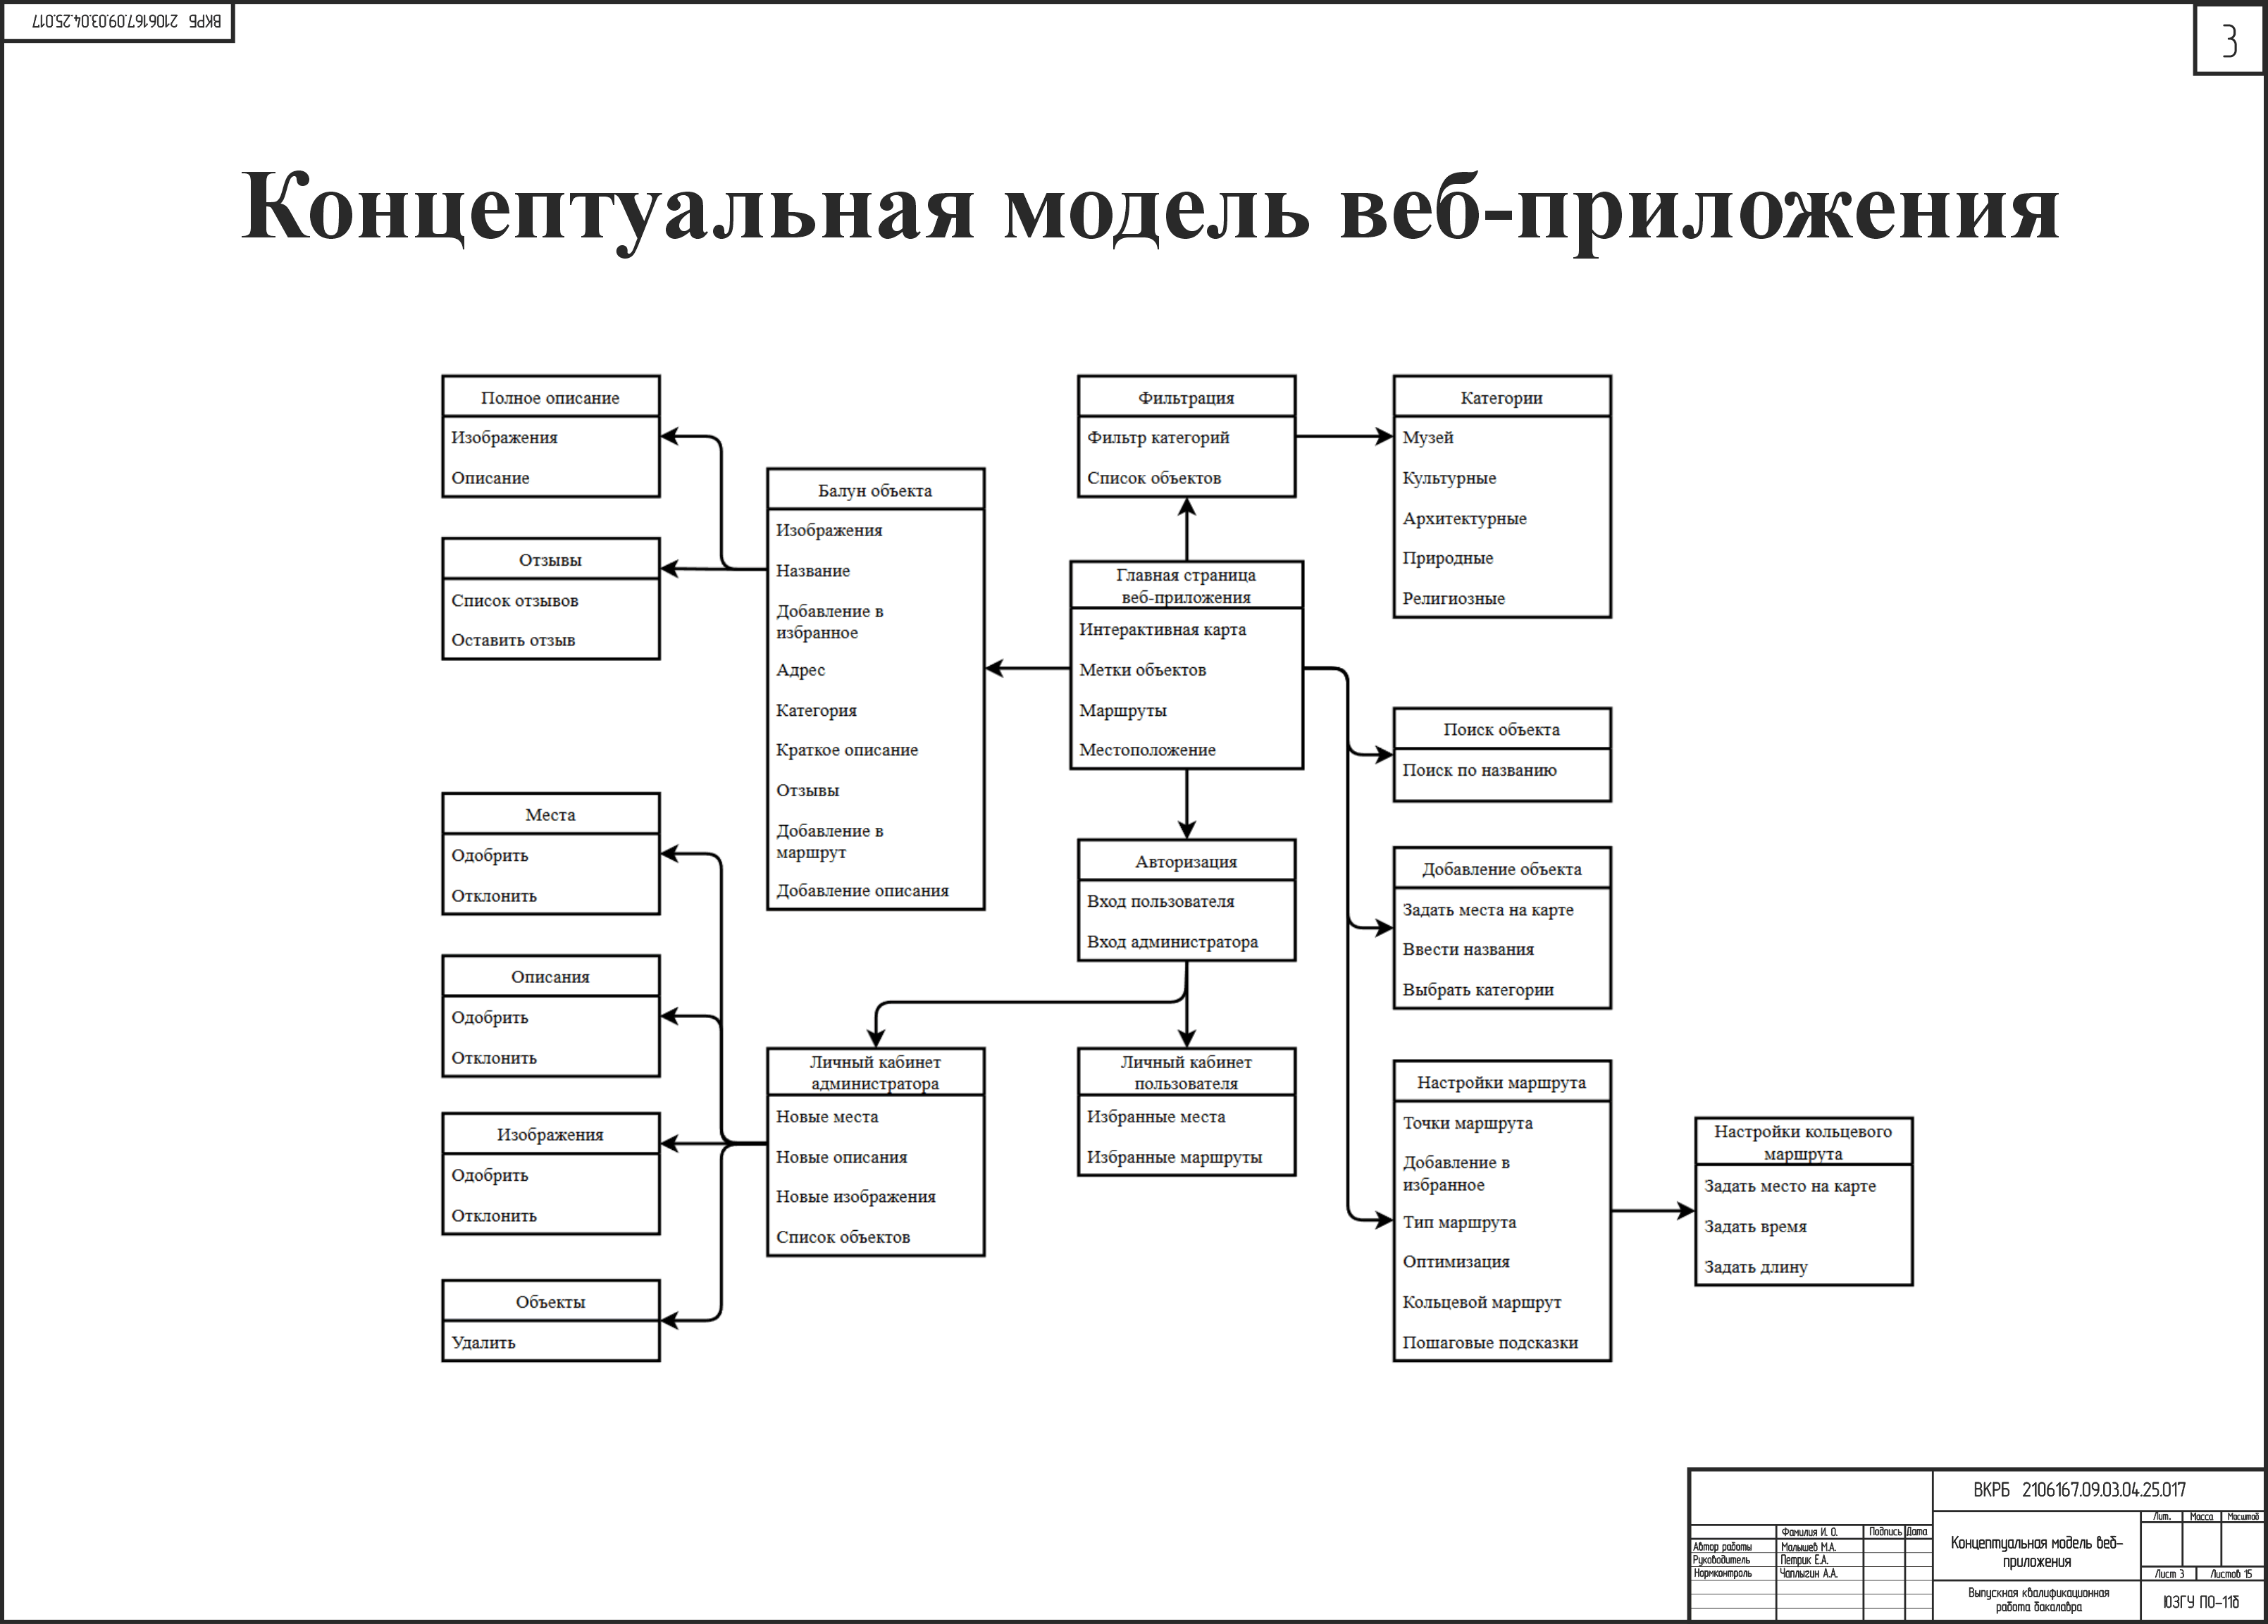
\includegraphics[width=0.82\linewidth]{плакат3.png}
    \заголовок{Концептуальная модель сайта}
    \label{pl3:image}      
\end{плакат}

\begin{плакат}
    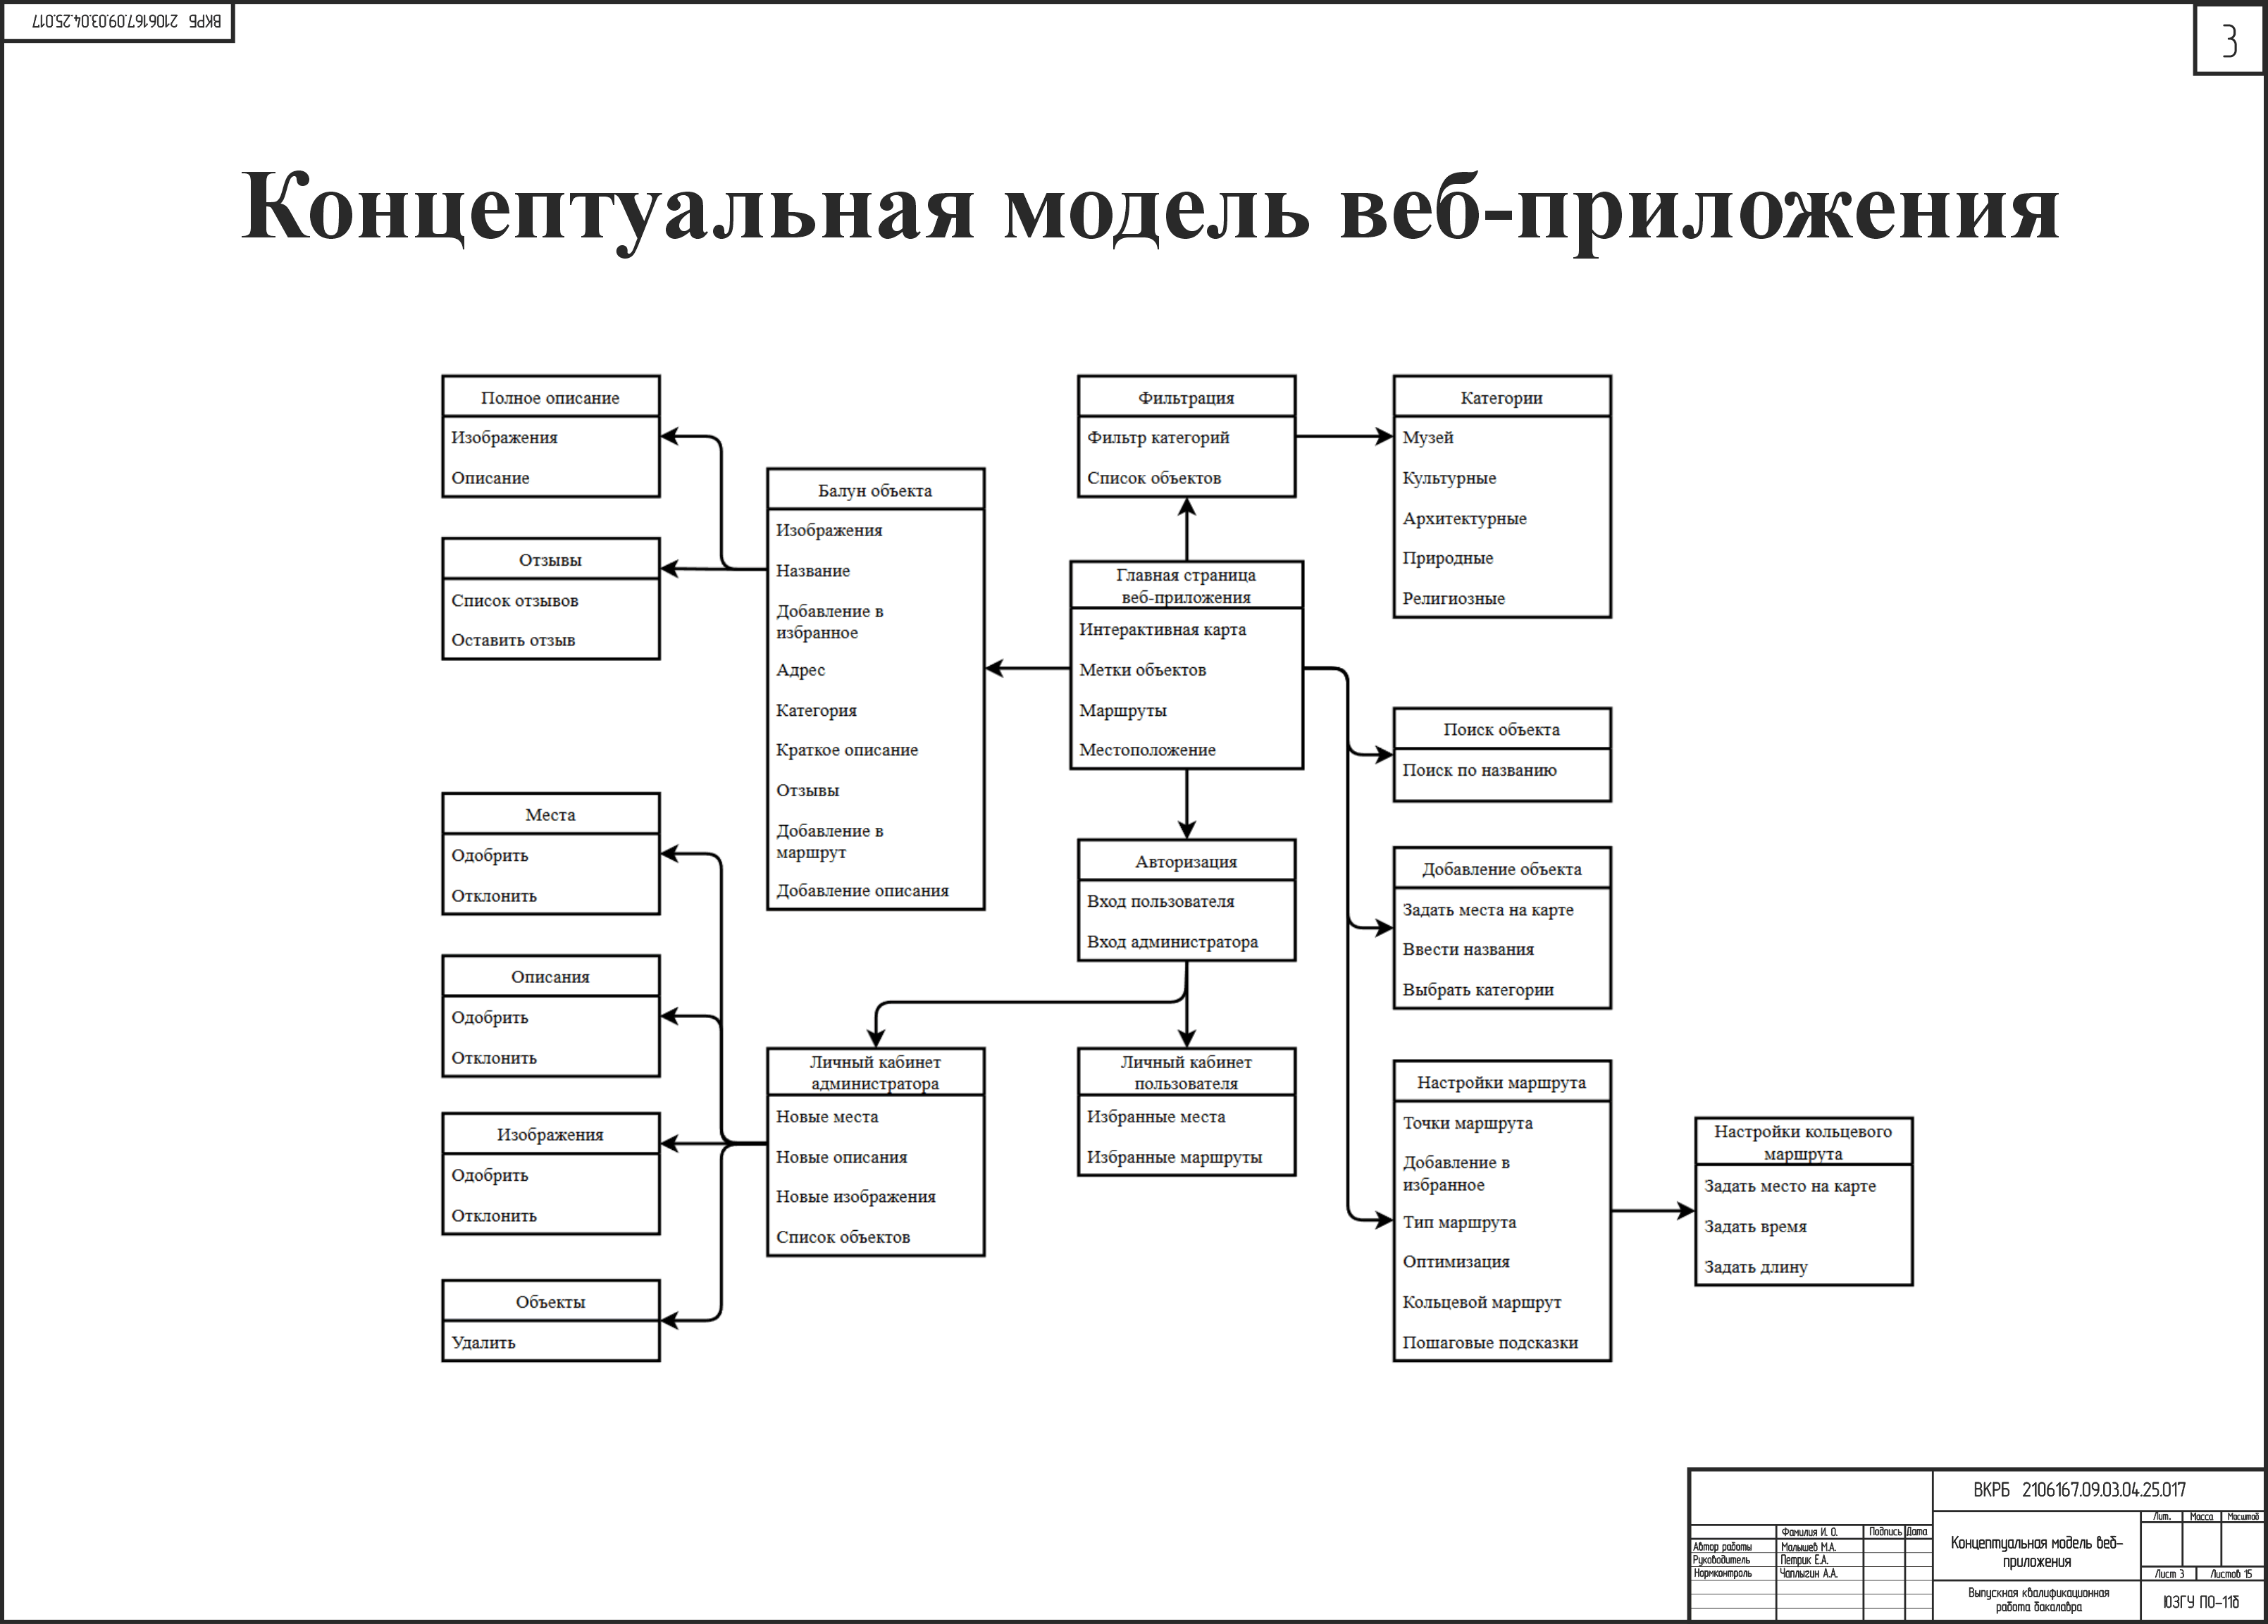
\includegraphics[width=0.82\linewidth]{плакат3.png}
    \заголовок{Еще плакат}
    \label{pl4:image}      
\end{плакат}

\end{landscape}
}\fi
\ifПрактика{}\else{\appendix{Фрагменты исходного кода программы}

openFilterMenu.js
\lstinputlisting[language=JavaScript, frame=none]{openFilterMenu.js}

openObjectInformationMenu.js
\lstinputlisting[language=JavaScript, frame=none]{openObjectInformationMenu.js}

openRegistrationMenu.js
\lstinputlisting[language=JavaScript, frame=none]{openRegistrationMenu.js}

openRouteMenu.js
\lstinputlisting[language=JavaScript, frame=none]{openRouteMenu.js}

openSearchMenu.js
\lstinputlisting[language=JavaScript, frame=none]{openSearchMenu.js}

routeHandler.js
\lstinputlisting[language=JavaScript, frame=none]{routeHandler.js}

addData.js
\lstinputlisting[language=JavaScript, frame=none]{addData.js}

addObject.js
\lstinputlisting[language=JavaScript, frame=none]{addObject.js}

addObjectInformation.js
\lstinputlisting[language=JavaScript, frame=none]{addObjectInformation.js}

addObjectPicture.js
\lstinputlisting[language=JavaScript, frame=none]{addObjectPicture.js}

addReview.js
\lstinputlisting[language=JavaScript, frame=none]{addReview.js}

deletePoint.js
\lstinputlisting[language=JavaScript, frame=none]{deletePoint.js}

favoritePoint.js
\lstinputlisting[language=JavaScript, frame=none]{favoritePoint.js}

Filter.js
\lstinputlisting[language=JavaScript, frame=none]{Filter.js}

loadFavoritesPoints.js
\lstinputlisting[language=JavaScript, frame=none]{loadFavoritesPoints.js}

loadFavoritesRoutes.js
\lstinputlisting[language=JavaScript, frame=none]{loadFavoritesRoutes.js}

Location.js
\lstinputlisting[language=JavaScript, frame=none]{Location.js}

openAccountMenu.js
\lstinputlisting[language=JavaScript, frame=none]{openAccountMenu.js}

openAddMenu.js
\lstinputlisting[language=JavaScript, frame=none]{openAddMenu.js}

get\_point\_name.php
\lstinputlisting[language=php, frame=none]{get_point_name.php}

get\_reviews.php
\lstinputlisting[language=php, frame=none]{get_reviews.php}

index.php
\lstinputlisting[language=php, frame=none]{index.php}

login.php
\lstinputlisting[language=php, frame=none]{login.php}

logout.php
\lstinputlisting[language=php, frame=none]{logout.php}

moderate.php
\lstinputlisting[language=php, frame=none]{moderate.php}

register.php
\lstinputlisting[language=php, frame=none]{register.php}

save\_object.php
\lstinputlisting[language=php, frame=none]{save_object.php}

save\_point.php
\lstinputlisting[language=php, frame=none]{save_point.php}

save\_route.php
\lstinputlisting[language=php, frame=none]{save_route.php}

send\_review.php
\lstinputlisting[language=php, frame=none]{send_review.php}

add\_object.php
\lstinputlisting[language=php, frame=none]{add_object.php}

auth.php
\lstinputlisting[language=php, frame=none]{auth.php}

check\_favorite.php
\lstinputlisting[language=php, frame=none]{check_favorite.php}

check-auth.php
\lstinputlisting[language=php, frame=none]{check-auth.php}

data.php
\lstinputlisting[language=php, frame=none]{data.php}

db.php
\lstinputlisting[language=php, frame=none]{db.php}

db\_connect.php
\lstinputlisting[language=php, frame=none]{db_connect.php}

delete\_point.php
\lstinputlisting[language=php, frame=none]{delete_point.php}

delete\_route.php
\lstinputlisting[language=php, frame=none]{delete_route.php}

functions.php
\lstinputlisting[language=php, frame=none]{functions.php}

get\_favorite\_points.php
\lstinputlisting[language=php, frame=none]{get_favorite_points.php}

get\_favorite\_routes.php
\lstinputlisting[language=php, frame=none]{get_favorite_routes.php}

get\_images.php
\lstinputlisting[language=php, frame=none]{get_images.php}

\ifВКР{
\newpage
\addcontentsline{toc}{section}{На отдельных листах (CD-RW в прикрепленном конверте)}
\noindent
\begin{tabular}{p{5.8cm}C{4.8cm}C{4.8cm}}
   Автор ВКР & \lhrulefill{\fill} & \fillcenter\Автор \\
            \setarstrut{\footnotesize}
           & \footnotesize{(подпись, дата)} & \\
            \restorearstrut
   Руководитель ВКР & \lhrulefill{\fill} & \fillcenter\Руководитель \\
            \setarstrut{\footnotesize}
           & \footnotesize{(подпись, дата)} & \\
            \restorearstrut
   Нормоконтроль & \lhrulefill{\fill} & \fillcenter\Нормоконтроль \\
            \setarstrut{\footnotesize}
           & \footnotesize{(подпись, дата)} & \\
            \restorearstrut
\end{tabular}
\vskip 2cm
\begin{center}
\textbf{Место для диска}
\end{center}
}\fi
}\fi
\end{document}
